% !TEX root = _main.tex
%\title{旋律化されたことばの表現構造の分析}
%\author{32045036　佐々木　美音}{SASAKI Mio}{FUKU}[]
% ==========================================
% ここから本文．あとは各自で
% ==========================================

%1
\section{はじめに}
人々は古来より，思いを様々な方法で「言葉」に乗せ，「うたう」という行為を通じて伝えてきた．
%その方法の中でも，文字で伝えるということに着目したい．文字で伝える方法には，手紙など書いて伝える，口に出して言葉で伝える，歌で伝えるといった方法がある．
%本研究では，
%
%古来より，「うたう」という行為はなされていた．
例えば，紀元前3000年頃に生まれたとされる古代エジプト文明では，既に歌手という存在がいることが確認されている\cite{eziputo}．また日本でも，三国志の魏志倭人伝に「歌舞」の記載があり，少なくとも3世紀末ごろには「うたう」という概念があったことがわかる\cite{gisiwazinden}．\par
%\red{見出しでいうほど「歴史」の話になってない（３世紀で終わり？）}\red{削るか迷ってます　ささき}
%「うたう」行為にはさまざまな漢字表記が存在する\cite{kozien}．例を以下に示す．
%\red{このように，「うたう」という言葉は感情・芸術表現を表すものであり，}
%\red{「うたう」行為にはさまざまな漢字表記があって，感情・芸術表現の展開がたくさんある（歌，唄，詩，詠，朗，謳，揺...）ことについて言及する．「ことばを音で伝える」こと自体はいろんな表現手段がある．文字としての言葉を考えるか，音としての言葉を考えるか，本研究がどちらに興味を持っているのかに話をつなげていく．それに合わせて，下の段落もつながるように}\par
%\red{以下修正↓}\par
では，現在「うたう」という行為はどのような表現があるのだろうか．広辞苑\cite{kozien}によると，「うたう」に関連する語句は以下のような意味がある．
\begin{itemize}
  \item 歌---うたう，うた
  \item 唄---うたう，うた（三味線伴奏の邦楽）
  \item 詩---うた（近代詩・現代詩，まれに）
  \item 謡---うたう，うたい（能・狂言）
  \item 吟---きんずる（詩歌などをうたう）
  \item 詠---（うた）よみ（和歌を詠む）
  \item 謳---うたう，うたわれる（世間からもてはやされる）
\end{itemize}
このように，「うたう」には感情・芸術表現としての意味が多数ある．これらをさらに大別すると，
\begin{itemize}
  \item 音としての言葉を伝える
  \item 文字としての言葉を伝える
\end{itemize}
の2つに大別される．%\red{↑ここまで}\par
%\red{私は？著者は？本研究は？}この中でも，音としての言葉を伝える，という意味としての「うたう」に着目する．
%（歌，唄，詩，詠，朗，謳，揺...）ことについて言及する
% \red{言葉を}伝える方法には，手紙など\red{文章にして書く}，口に出して\red{声や歌}で伝えるといった方法がある．
% %言葉で伝える，歌で伝えるという二つに着目したい．二つとも，「口に出して，言葉で伝える」ということは一致しているが，表現方法は異なる．
% \red{とくに「声や歌で伝える」という表現方法は，}
% %この二つの表現方法は、

いずれにしても，「うたう」という行為は，%どちらも
「音」を通じて情報や感情を伝える手段として用いられる。しかし、発話は主に会話や朗読の場で情報伝達や感情表現を目的とするのに対し、歌は旋律やリズムを伴うことで芸術的要素を持ち、より感情やメッセージを強調する手段となる。このように、共通点がありつつも異なる性質を持つ発話と歌について、より詳細に分析する必要がある．

本研究では，発話表現と歌の表現を，「音での表現」という観点から比較し，両者に違いがあるのかを検討する．




%2
\section{ことばから創出する旋律表現}

%2.1
%\subsection{ことばと音の歴史}
%古来より，「うたう」という行為はなされていた．例えば，紀元前3000年頃に生まれたとされる古代エジプト文明では，既に歌手という存在がいることが確認されている\cite{eziputo}．また日本でも，三国志の魏志倭人伝に「歌舞」の記載があり，少なくとも3世紀末ごろには「うたう」という概念があったことがわかる\cite{gisiwazinden}．
%\red{見出しでいうほど「歴史」の話になってない（３世紀で終わり？）}\red{削るか迷ってます　ささき}


%2.2
\subsection{日本語の音韻と旋律の関係}\label{sec:2.2}
メロディと歌詞の関係について，堤らの研究\cite{tutumi}，米林らの研究\cite{orpheus}が挙げられる．\par
%（おじさんの歌えない歌）
米林らは，歌唱曲の自動作曲システムOrpheusを開発した．これはWebブラウザ上で日本語の歌詞テキストを入力し，作曲のパラメータを選択すると，歌詞の韻律に基づいて自動作曲が行われ，伴奏付きの合成歌唱音声と楽譜が出力される，といったシステムである．このシステムで旋律生成をする際，原則として歌詞の韻律と旋律の上下が一致することが必要であるとしている．
%（日本語の音韻と旋律の関係について）
堤らは，童謡・唱歌について，メロディの音程と歌詞の音韻の音程との関係を調査・分析している．この研究では，童謡・唱歌の中で，歌詞の音韻の音程が高低する箇所とメロディの音程の高低とがマッチしていることが結果としてわかっている．これにより，これらのジャンルではメロディと歌詞の音程一致度が比較的高いため，童謡や唱歌は歌いやすいのではないか，という考察がなされている．

米林，堤の研究を通じ，歌唱曲を作成する際に歌詞の韻律が大事になってくること，また，ことばと旋律の関係において，特定のジャンルでのメロディと歌詞の音程一致度が高いことがわかっている．

%2.3
\subsection{同一歌詞に対する旋律表現}\label{sec:2.3}
本研究の直接的な先行研究として，塩見の研究\cite{sikukara}がある．この研究では，共通の歌詞（フレーズ）を歌唱するとき，どの語がどんな音の長さ，高さで歌われているかを分析し，どのような傾向で歌われるかを明らかにすることを目的としている．\par%特定のフレーズがどのように歌われる傾向にあるかを，様々な観点から検証している．
%\red{表面的にやったことを述べるだけでなく，どういう考え方や狙いがあって下記を調べたものなのかを読者に理解させる}\par


考察されていた点は以下の通りである．%\red{箇条書きで誤魔化さないこと}

\begin{itemize}
  \item 一語に対する歌音の長さ
        \begin{itemize}
          \item フレーズ全体の発音時間（拍）
          \item 「あなたに」「あいたくて」がそれぞれ占める時間（拍）の割合
          \item 「あなたに」の中での音の長さ（拍）の割合
          \item 「あいたくて」の中での音の長さ（拍）の割合
          \item 1音単位の発音時刻（拍）と拍節との関係
        \end{itemize}
  \item 一語に対する音高の比較
        \begin{itemize}
          \item フレーズ全体の音域
          \item フレーズ全体の発音時間（拍）と音高の関係
          \item フレーズ全体の発音時間（拍）を相対的に見た時の音高推移
        \end{itemize}
  \item 一語に対する音程の比較
        \begin{itemize}
          \item 相対時間（拍）での比較
          \item 冒頭「あ」を起点とする音程推移
          \item 同曲中のフレーズについての音高比較
        \end{itemize}
\end{itemize}
また，考察内容は以下の通りである．
\begin{itemize}
  \item 言葉に対する音の長さ
  \item 「あなたにあいたくて」の言葉の解釈
  \item 楽曲中のフレーズの役割（意味的な）との関係
\end{itemize}
この通り，先行研究では主に拍を基準として各種プロットを行っている．また，考察は主に目視で行っている．




%2.3
\subsection{本研究の狙い}
%\red{先行研究を踏襲したものであることを言及したい．堤さんの論文の書き方を見倣ってください}

%\cut{\ref{sec:2.2}節で挙げたように，}世の中にはことばと音に関しての研究が数多くある．しかし，ことばと歌そのものを比較した研究は少ない．\par
%\red{また，}塩見の研究\cite{sikukara}はことばと歌そのものを比較した研究である\red{．}
%が，秒数（絶対時間）に対応していない，単なる比較である点など，まだ分析の余地がある．
本研究は，前節の塩見による研究を基盤として発展させるものである．塩見は「あなたにあいたくて」の開始地点からどのように音高が推移していくか，また，「あなたに」「あいたくて」と，分解しての拍の割合を見たりと，単一フレーズ同士での比較，相対的な単位である拍の比較を行っていた．\par
本研究では，塩見による研究では行っていなかった，発話表現と歌唱表現との比較を主に行っていく．また，塩見の研究では拍単位での比較であったが，本研究では，秒数（実時間）換算した発話表現・歌唱表現との比較も取り入れた．また，新たな研究対象フレーズを追加し，研究の拡張を行った．
%発話表現と歌の表現を，「音での表現」という観点から比較し，両者に違いがあるのかを考察していく．\par
先行研究との詳しい違いを\tabref{tab:tigai}に示す．


\begin{table}[t]
  \centering
  \scriptsize
  \caption{先行研究との違い}
  % !TEX root = _main.tex

\begin{tabular}{c|cc} \hline
               & 先行研究\cite{sikukara} & 本研究                            \\ \hline\hline
    対象フレーズ     & 「あなたにあいたくて」         &
    \begin{tabular}{c}
        (a)「あなたにあいたくて」 \\(b)「ひかりのほう」
    \end{tabular}                                       \\ \hline
    収録曲数       & 103曲131フレーズ        &
    \begin{tabular}{l}
        (a)128曲188フレーズ \\ (b)153曲265フレーズ
    \end{tabular}                                           \\ \hline
    楽譜データ      & MusicXML            & \begin{tabular}{c}
                                           MusicXML \\\scriptsize{（BPMあり}）
                                       \end{tabular} \\ \hline
    楽曲メタデータ    &
    \begin{tabular}{c}
        歌唱者情報 \\作詞・作曲者\\歌詞\\ \\
    \end{tabular}
               &
    \begin{tabular}{c}
        歌唱者情報 \\作詞・作曲者\\歌詞\\ 性別・グループ有無\\発売年日
    \end{tabular}              \\ \hline
    プロット方法     & matplotlib          & PlotlyおよびDash                  \\ \hline
    分析対象 &
    \begin{tabular}{c}
        歌音の長さ \\音高\\音程
    \end{tabular}
               &
    \begin{tabular}{c}
        発話 \\男女間\\年代別\\表拍・裏拍
    \end{tabular}                       \\ \hline
\end{tabular}

  \label{tab:tigai}
\end{table}

%\footnotetext{\red{「ひかりのほう」に関しては，補完ではなく新規に集めたのでは？何を比較しているのかがわかりにくい．→線書かないと変に見えるので付け足しました ささき}}
%3
%\section{研究概要}
\section{分析手法}

%3.2
\subsection{歌詞の選定}\label{sec:3.2}

%3.2.1
まず，研究対象になる歌詞の選定から行う．
先行研究（\ref{sec:2.3}節）では，下記の基準に沿って\textbf{「あなたにあいたくて」}を採用していた．

\begin{enumerate}
  \renewcommand{\labelenumi}{\arabic{enumi})}
  \item ひとつの単語だけでなく，名詞や助詞，動詞が含まれること．（複数の単語を組み合わせたフレーズを用いることで，拍子の変化や音の高さの変化に特徴が現れやすいと思われるためである）
  \item フレーズから想起される文脈がある程度一般的であること．
  \item 日本の楽曲で少なくとも100 曲は歌われていること．
\end{enumerate}

本研究では，これに加え，新たに\textbf{「ひかりのほう」}を採用する．採用理由としては，上記の基準を満たしていることに加え，
\begin{itemize}
  \item 各単音の重複がないこと
        \begin{itemize}
          \item 「あなたにあいたくて」では「あ」と「た」が重複して出現しており，プログラムが少し煩雑になっていた
        \end{itemize}
  \item カバー楽曲が少ないこと
        \begin{itemize}
          \item 楽曲数が多くても，カバー楽曲の割合が多ければ似たようなフレーズの形が頻出して偏りが出てしまうため，本研究では多くとも2回以下の出現頻度のものを探した
        \end{itemize}
\end{itemize}
これらの条件を満たしているため，本研究での採用となった．

%3.1
\subsection{分析対象（旋律）}\label{sec:3.1}
本研究で分析対象となる，楽譜から抽出する音楽の要素を\tabref{tab:bunseki_info}に示す．

% !TEX root = _main.tex

\begin{table}[tb]
    \centering
    \caption{分析に用いる旋律情報およびメタデータ}
    \label{tab:bunseki_info}
    \begin{tabular}{c|c|l}
        \hline
                                         & 項目\cut{名}  & 説明\red{\scriptsize{※具体的な変数や型で示すべし}}                    \\ \hline
        \multirow{10}{*}{\pbox<t>{旋律情報}} & \red{歌詞}   & \red{分析に必要\scriptsize{（説明になってない）}}                     \\
                                         & \red{楽曲ID} & \red{楽曲名}＋同曲内の出現\red{順}                                \\
                                         & BPM        & \red{四分音符単位でのテンポ\scriptsize{（\ref{sec:gakufu_data}節）}} \\%秒数・累積秒に必要
                                         & 拍子         & \red{分析に必要\scriptsize{（説明になってない）}}                     \\
                                         & 調号         & \red{分析に必要\scriptsize{（説明になってない）}}                     \\
                                         & 音符の種類      & 音符\red{ または }休符\cut{か} \footnotemark                   \\
                                         & \red{音高}   & \red{MIDIノートナンバー}                                      \\
                                         & \red{開始時刻} & \red{開始音の拍の位置\footnotemark}                            \\
                                         & 拍数・累積拍     & \red{相対時間の基準(?)\footnotemark}                          \\
                                         & 秒数・累積秒     & \red{絶対時間の基準(?)}                                       \\
        \hline
        \multirow{5}{*}{\pbox<t>{メタデータ}} & \red{楽曲ID} & \red{楽曲名}＋同曲内の出現\red{順}                                \\
                                         & \red{歌手名※} & \multirow{3}{*}{\begin{tabular}{l}
                                                                                ※同じフレーズを複数の曲で \\
                                                                                使用しているか\end{tabular} }                 \\
                                         & 作詞者※       &                                                        \\
                                         & 作編曲者※      &                                                        \\
                                         & \red{歌手属性} & 男女，グループかどうか                                            \\
                                         & 発売日        & 発売年ごとの傾向の分析                                            \\ \hline
    \end{tabular}

\end{table}


\footnotetext{\red{休符は文字に対応しないと思うけど，分析対象として使ってるの？}}
\footnotetext{\red{offsetは「``曲の開始"からの拍の長さ」ではないと思うよ..}}
\footnotetext{\red{「拍」や「秒」が「基準」と言われてもよくわからない．}}


また，楽譜データとは別に楽曲のメタデータを作成した．内容は以下の通りである．\par
% \begin{musequote}
%   \begin{itemize}
%     \item アーティスト・作詞・作編曲者：同じフレーズを複数回使用しているアーティストはいるのか
%     \item 歌い手：男女，グループかどうか
%     \item 発売日：発売年ごとの傾向の分析
%   \end{itemize}
% \end{musequote}
抽出した楽譜のデータとメタデータ，それぞれにIDを付けることによって，連動して分析を行うことができる．

%3.2.2
\subsubsection{選定歌詞を含む楽曲情報の収集}\label{sec:3.2.2}
音楽的要素を抽出するため，まず楽曲の楽譜データの作成を行う．手順を以下に示す．楽譜データの形式にはMusicXML\cite{musicxml}を使用した．



先行研究では，「あなたにあいたくて」を含む楽曲が157曲見つかっていた．「ひかりのほう」を含む楽曲については，歌ネット\cite{utanet}を参考に，2024年10月15日までで合計183曲見つかった．このうち，表記揺れを含む内訳は以下の通りである．
\begin{itemize}
  \item 「光の方」…151曲
  \item 「光のほう」…24曲
  \item 「ひかり（ヒカリ）の方」…4曲
  \item 「ひかり（ヒカリ）のほう」…4曲
\end{itemize}
本研究では，これらの表記揺れも含めた全ての楽曲を対象とする．
%以上の歌詞の選定により，「あなたにあいたくて」の含まれる楽曲157曲，「ひかりのほう」の含まれる楽曲185曲を対象に，以下の作成方法で歌詞フレーズを収集する．



\begin{figure*}[t]
  %\caption{楽譜の変換の対応例}
  \begin{minipage}{1.0\hsize}
    \CaptionType{figure}
    \centering
    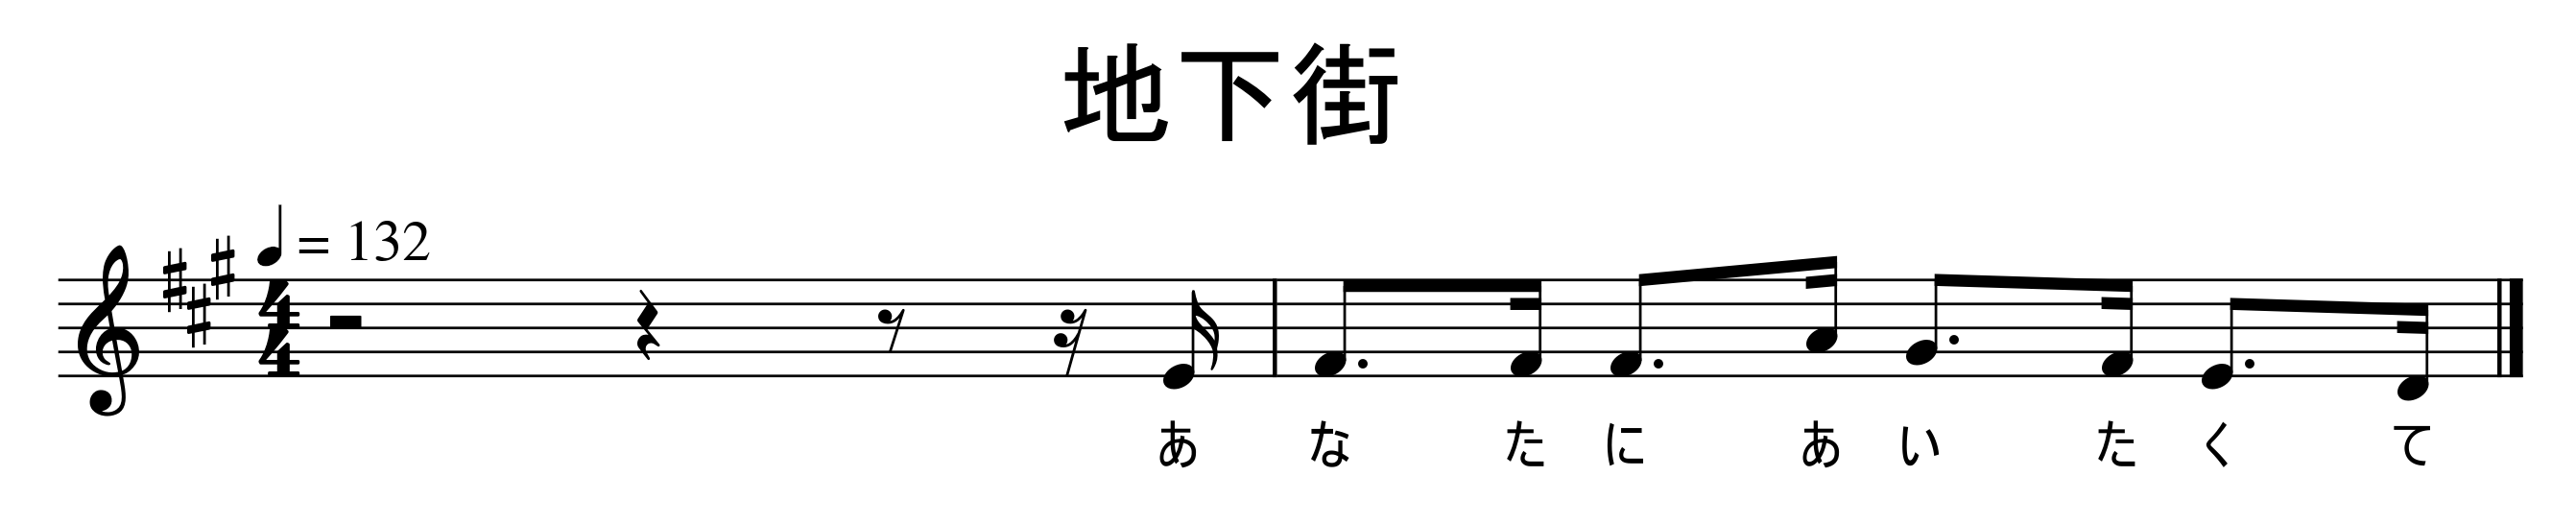
\includegraphics[width=.7\columnwidth]{fig/gakuhu.png}
    \caption{“あなたにあいたくて”フレーズの楽譜例}
    \label{gakuhu}
  \end{minipage}
  \vspace{12pt}
  \begin{minipage}{1.0\hsize}
    \CaptionType{table}
    \caption{楽譜と発音情報（quarterlength，オフセット）の対応関係}
    \centering
    \begin{tabular}{c|ccccccccc} \hline
      歌詞                  & あ    & な    & た    & に    & あ    & い    & た    & く    & て    \\ \hline\hline
      音符の種類               & 16   & 符点8  & 16   & 符点8  & 16   & 符点8  & 16   & 符点8  & 16   \\
      quarterlength       & 0.25 & 0.75 & 0.25 & 0.75 & 0.25 & 0.75 & 0.25 & 0.75 & 0.25 \\
      オフセット               & 3.75 & 4    & 4.75 & 5    & 5.75 & 6    & 6.75 & 7    & 7.75 \\
      オフセットを“あ”から数えなおしたもの & 0    & 0.25 & 1    & 1.25 & 2    & 2.25 & 3    & 3.25 & 4    \\ \hline
    \end{tabular}
    \label{quart}
  \end{minipage}
\end{figure*}

\begin{figure}[tb]
  \centering
  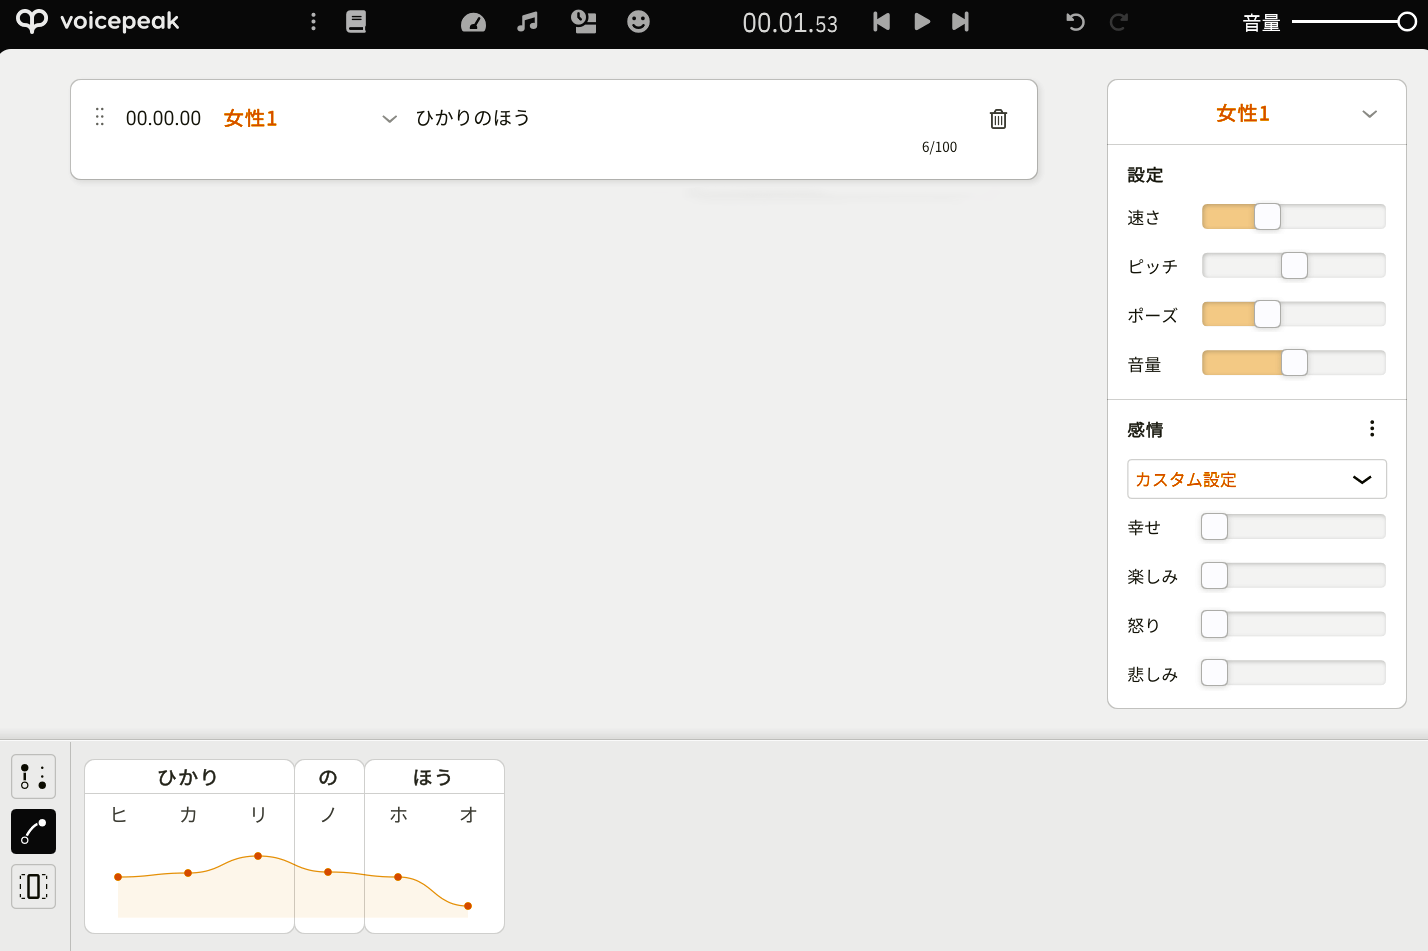
\includegraphics[width=\columnwidth]{fig/voicepeak.png}
  \caption{VOICEPEAKの操作画面}
  \label{voicepeak}
\end{figure}



\subsubsection{楽譜データの収集}
本研究では音楽表現を分析するため，各楽曲の旋律情報が必要である．そのため，分析対象となる各楽曲の楽譜を入手する必要がある．しかし，全ての対象楽曲において，楽譜データが公開されているとは限らない．そこで，本研究では，以下の方法を用いて楽譜データを収集する．
\begin{description}
  \item[(1)出版譜が流通している楽曲] 楽譜を入手後，楽譜制作ソフトを用い，当該フレーズ箇所の電子楽譜データを作成する．
  \item[(2)音源のみ視聴可能な楽曲] 音源を聴きながら 楽譜制作ソフトを用い，当該フレーズ箇所の電子楽譜データを作成する．
  \item[(3)どちらもできなかった楽曲] 本研究では対象外とする．
\end{description}


「あなたにあいたくて」については，先行研究で使用されていた103曲分131フレーズに加えて，新たに入手できた25曲分57フレーズを合わせ，合計128曲分188フレーズを本研究の分析対象とする．

「ひかりのほう」については，
全183曲中，19曲は音源が見つけられず，楽譜を作成することができなかった．また，楽譜は見つからず音源は見つかったが，該当箇所を楽譜に起こすことが難しかったものが11曲あったため，その11曲は除外をした．楽譜に起こせなかった理由としては，ラップ調や変拍子など，難解な楽曲であったため，データの正確性を考慮して除外した．\par
そのため聴取でき，かつ楽譜に起こすことのできた，合計153曲分265フレーズを本研究の分析対象とする．





%3.3
\subsection{発話イントネーション}\label{sec:3.3}
\ref{sec:2.2}で挙げた堤らの先行研究では，メロディの音程と歌詞の音韻の音程との関係を調査・分析している．その際，歌詞の音韻の音程の判定に使用していたのがアクセント辞書である．
本研究では，歌詞の音韻判定に用いるツールを，アクセント辞書からVOICEPEAK\cite{voicepeak}に変更し，発話のイントネーションを取得する．

%3.3.1
% \subsubsection{\red{基盤}ツール}
VOICEPEAK\cite{voicepeak}とは、株式会社 AHS によって開発・提供されている TTS(text to speech)の合成音声生成ソフトウェアであり，最新のAI音声合成技術を用い入力文字を読み上げるソフトである．\par
VOICEPEAK上で合成音声を作成する際，ユーザ側で任意にイントネーションや感情表現を変更することができるが，\figref{voicepeak}のように，VOICEPEAKはGUI操作のソフトとなっており，ユーザ側で数値として見ることが出来ない．そこで，VOICEPEAKのプロジェクトファイルを解析し，発話のイントネーション情報を取得していく．具体的な取得方法については，付録\ref{sec:huroku1}にて詳しく説明する．
%付録に飛ぶ


解析内容をもとに，それぞれのフレーズのイントネーションの最大値・最小値を100\%,0\%とし，割合を出した．割合については\ref{sec:3.4}節に示す．\par
分析では，このイントネーションの値をもとに，フレーズと発話イントネーションとの一致度も調べていく．


%3.4
\subsection{データセットの作成}\label{sec:3.4}
\ref{sec:3.2}節，\ref{sec:3.3}節で作成した楽譜データ，発話イントネーションのデータを元に，データセットを作成する．

%3.4.1
\subsubsection{楽譜データセット}\label{sec:gakufu_data}
MusicXMLをPython上で読み込む際に，music21\cite{music21}というライブラリを用いて変換を行った．
その際，音符の長さ（以下，音長とする）はmusic21の\verb|quarterlength|関数を用い，四分音符の長さをを1として変換した．例えば，\verb|quarterlength|を用いると，二分音符は2.0，符点八分音符は0.75となる．また，music21にはオフセットという指標もあり，これはフレーズの楽譜の開始からの四分音符の個数をカウントするものである．しかし，\figref{gakuhu}の場合だと小節の開始から歌いだされていない．そこで，歌詞の始点からオフセットを数えなおしたものを追加することにより，同じフレーズ間での比較がしやすくなる．
%
これらの対応関係について，\figref{gakuhu}および\tabref{quart}に示す．\par
またBPMを取得する際は，取得後に拍子記号と照らし合わせ，四分音符基準に換算をし直して取得した．例として\figref{onpu}を示す．

\begin{figure}[tb]
  \centering
  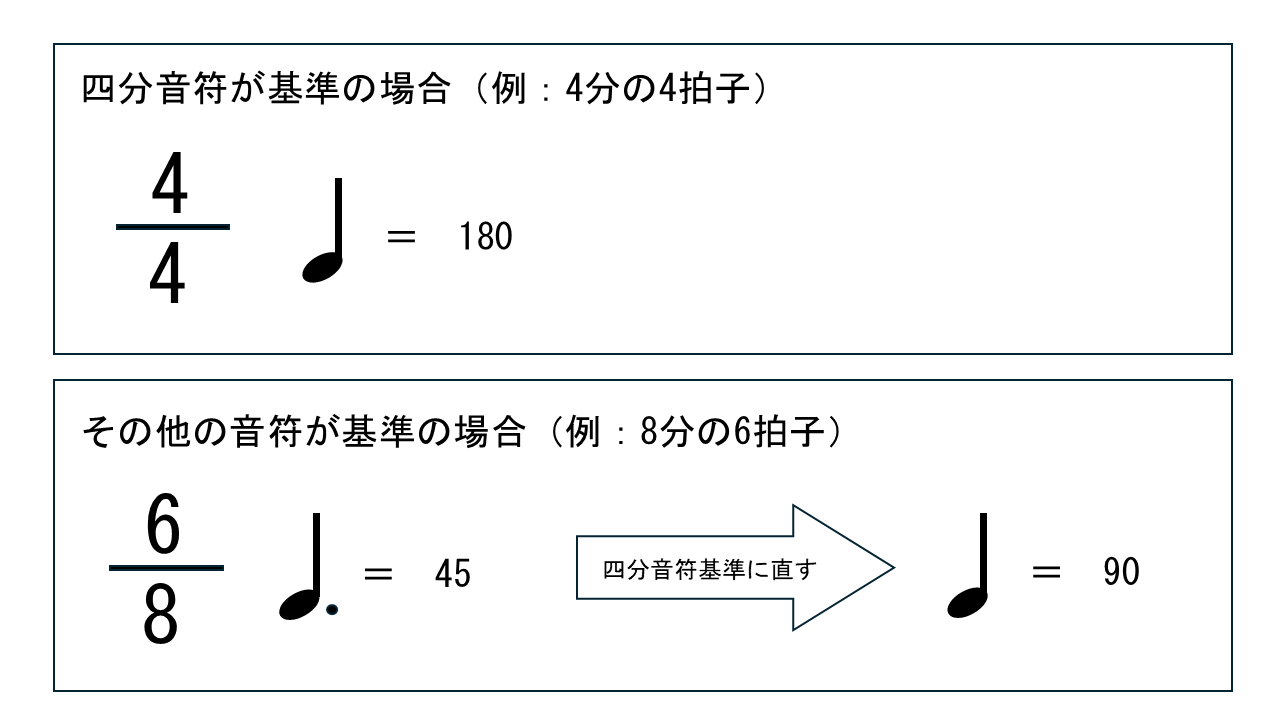
\includegraphics[width=.8\columnwidth]{fig/onpu.png}
  \caption{BPM変換の例}
  \label{onpu}
\end{figure}

%また，BPMを\red{取得}する際に，“八分音符=180”などの，四分音符基準でないBPMを取得してしまう．そのため，
%\begin{align*}
%\text{取得したBPM} \times
%\begin{split} \text{BPMの基準の音符}           \\
%\text{(＝の左側を四分音符に変換した数字)}
%\end{split}
%\end{align*}
%で算出した．“八分音符=180”だと，八分音符は四分音符を1とすると0.5となるため，\[180 \times 0.5 = 90\]となる．
%\red{式はちょっと無理があるので，もう少しわかりやすく書く．}

そのデータを CSVデータとして書き出した．変換のフローチャートは\figref{m_to_l}の通りである．また，実際に変換後の出力例を\figref{m_database}に示す．



%3.4.2
\subsubsection{発話イントネーションデータセット}\label{sec:3.4.2}
付録\ref{sec:3.3}で取得したデータをCSVに出力した．結果を\figref{intone_henkan}に示す．




\begin{figure}[tb]
  \centering
  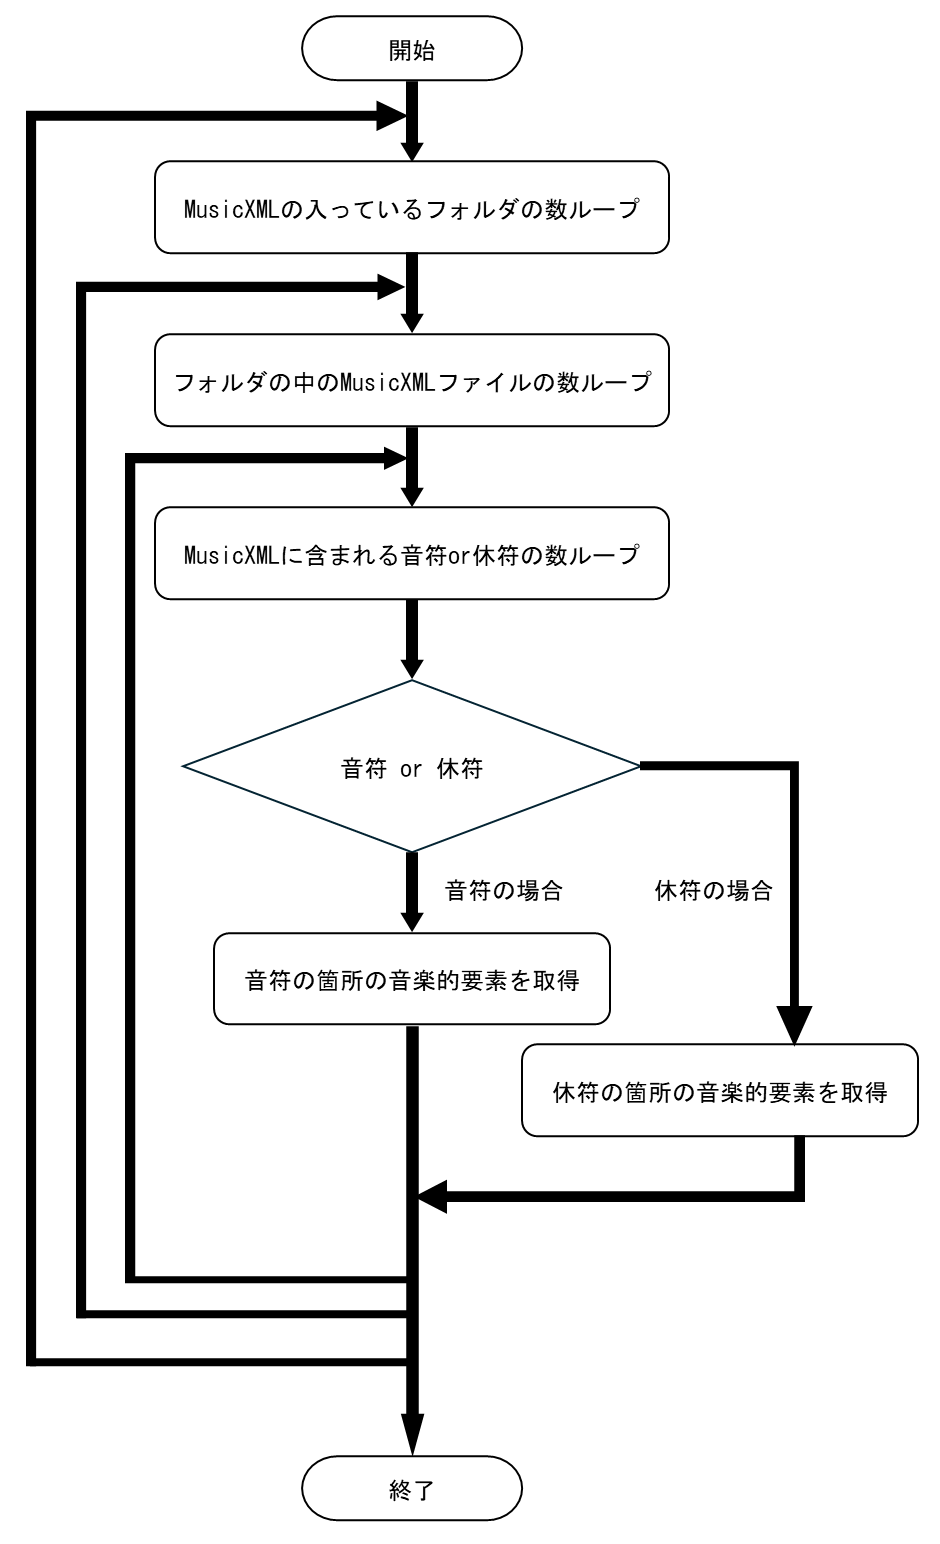
\includegraphics[width=\columnwidth]{fig/musicxml_to_csv_neo.png}
  \caption{MusicXMLからCSVファイルへの変換}
  \label{m_to_l}
\end{figure}
%\vspace{5mm}

\begin{figure}[tb]
  \centering
  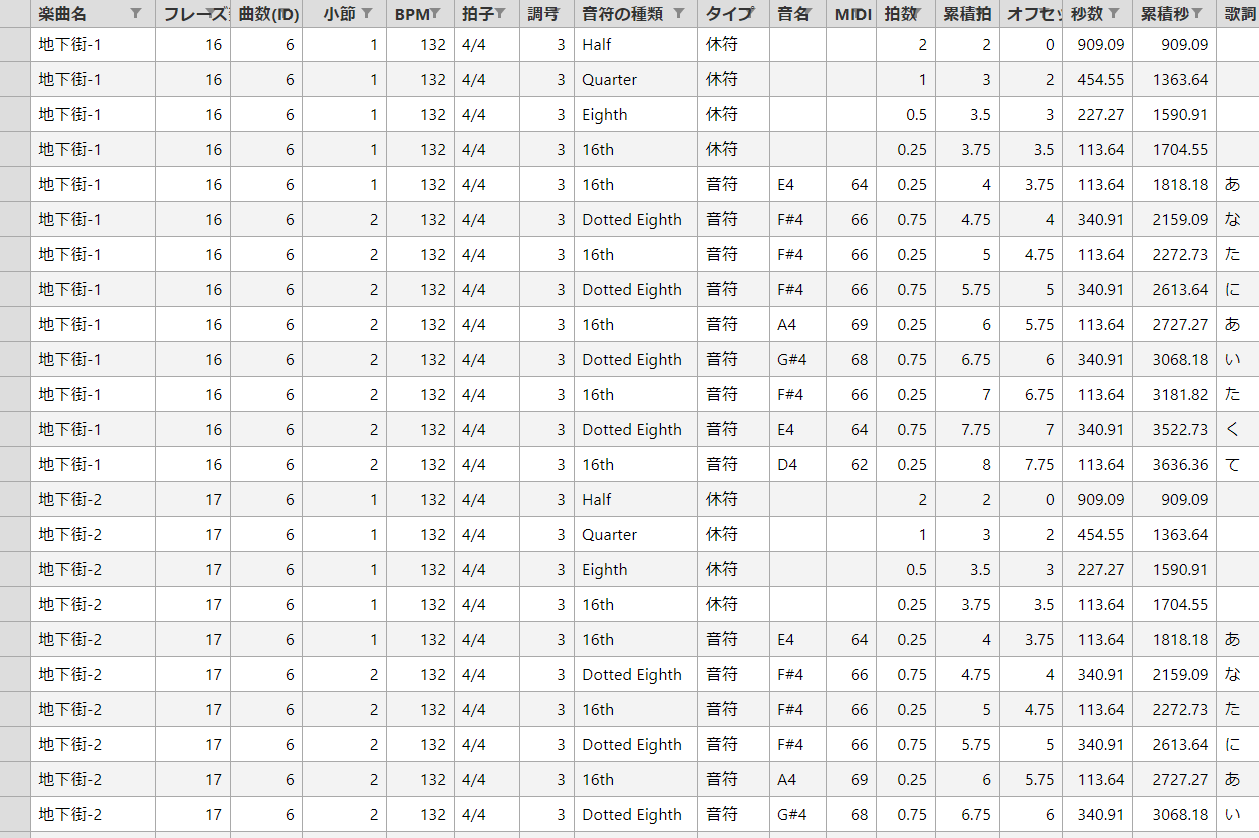
\includegraphics[width=\columnwidth]{fig/music_database.png}
  \caption{楽曲情報データベースの一部}
  \label{m_database}
\end{figure}


\begin{figure}[tb]
  \centering
  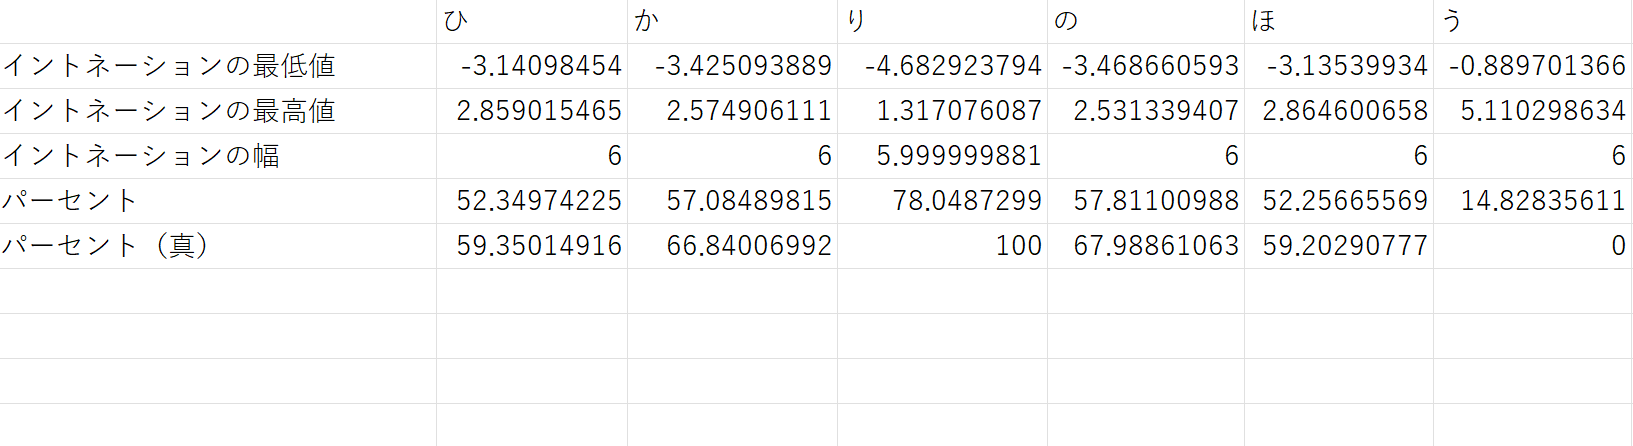
\includegraphics[width=\columnwidth]{fig/intone_henkan.png}
  \caption{“ひかりのほう”の発話イントネーションの割合}
  \label{intone_henkan}
\end{figure}

%3.4.3
\subsubsection{メタ情報セット}
\ref{sec:3.1}で記載したメタデータセットの情報取得は，アーティストの公式サイトや歌詞掲載サイトなどを閲覧し，手作業でExcelに入力した．また，歌い手の情報は，実際に楽曲を聴き，該当フレーズを歌っている人の性別・人数を確認し，Excelに入力した．\par
できたデータを\figref{meta}に示す．
\begin{figure}[tb]
  \centering
  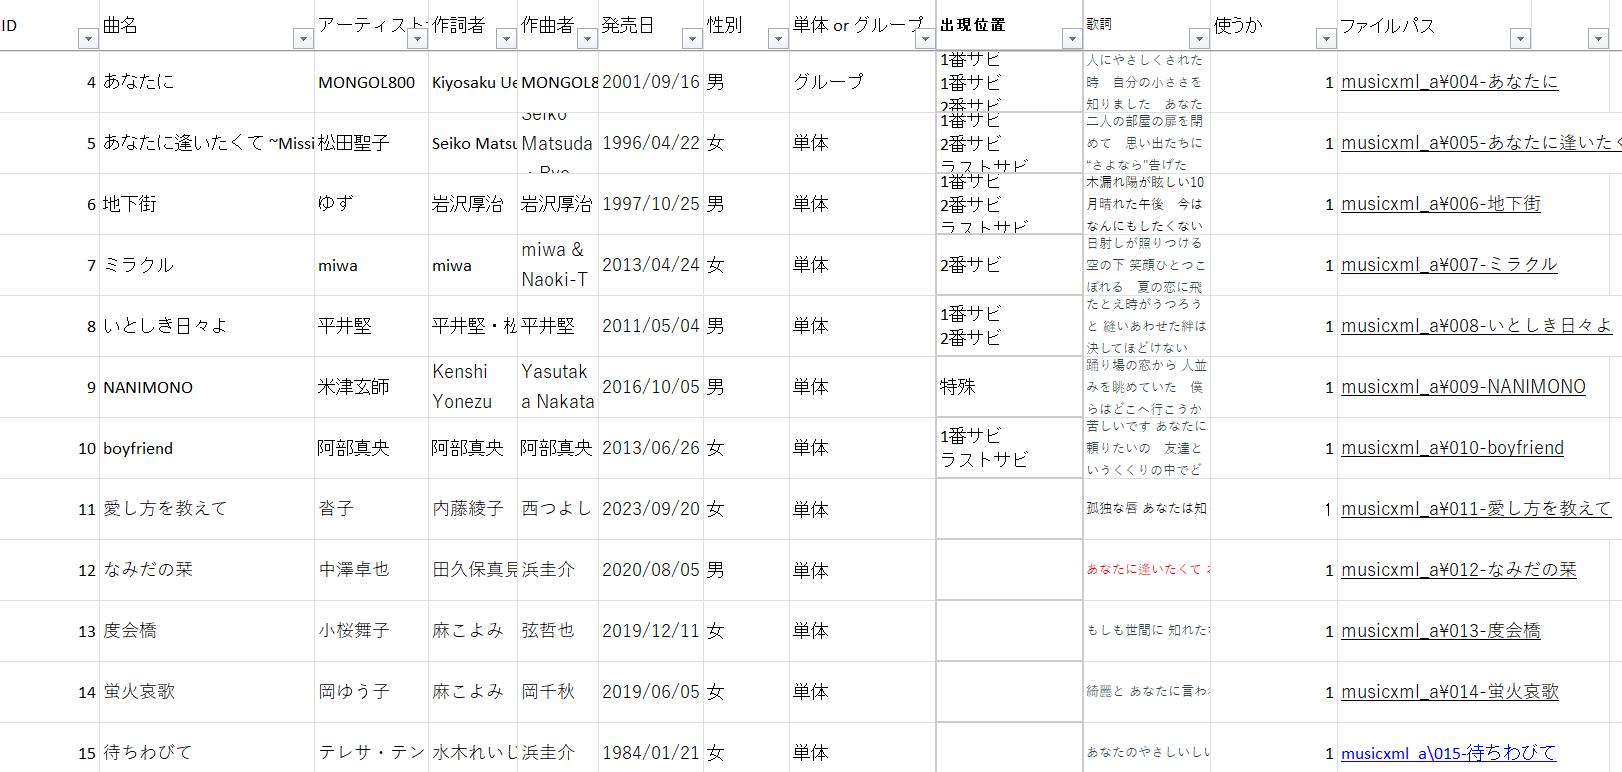
\includegraphics[width=\columnwidth]{fig/meta_dataset.png}
  \caption{メタ情報セットの一部}
  \label{meta}
\end{figure}

%3.5
\subsection{可視化ツール}
\ref{sec:3.4}で作成したデータセットを用い，可視化ツールの作成を行う．





\begin{figure*}[t]
  \centering
  \begin{minipage}{0.49\hsize}
    \centering
    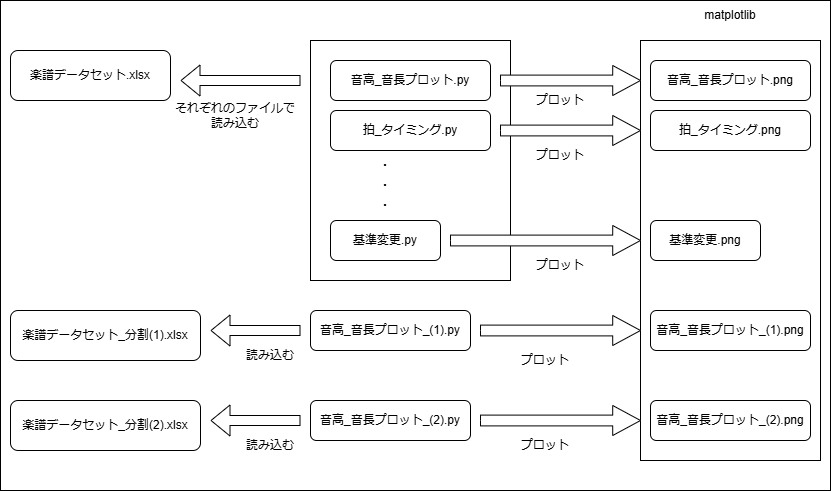
\includegraphics[width=\columnwidth]{fig/kyuufairu.png}
    \subcaption{システム構成}
    \label{kyuufairu}
  \end{minipage}
  \begin{minipage}{0.49\hsize}
    \centering
    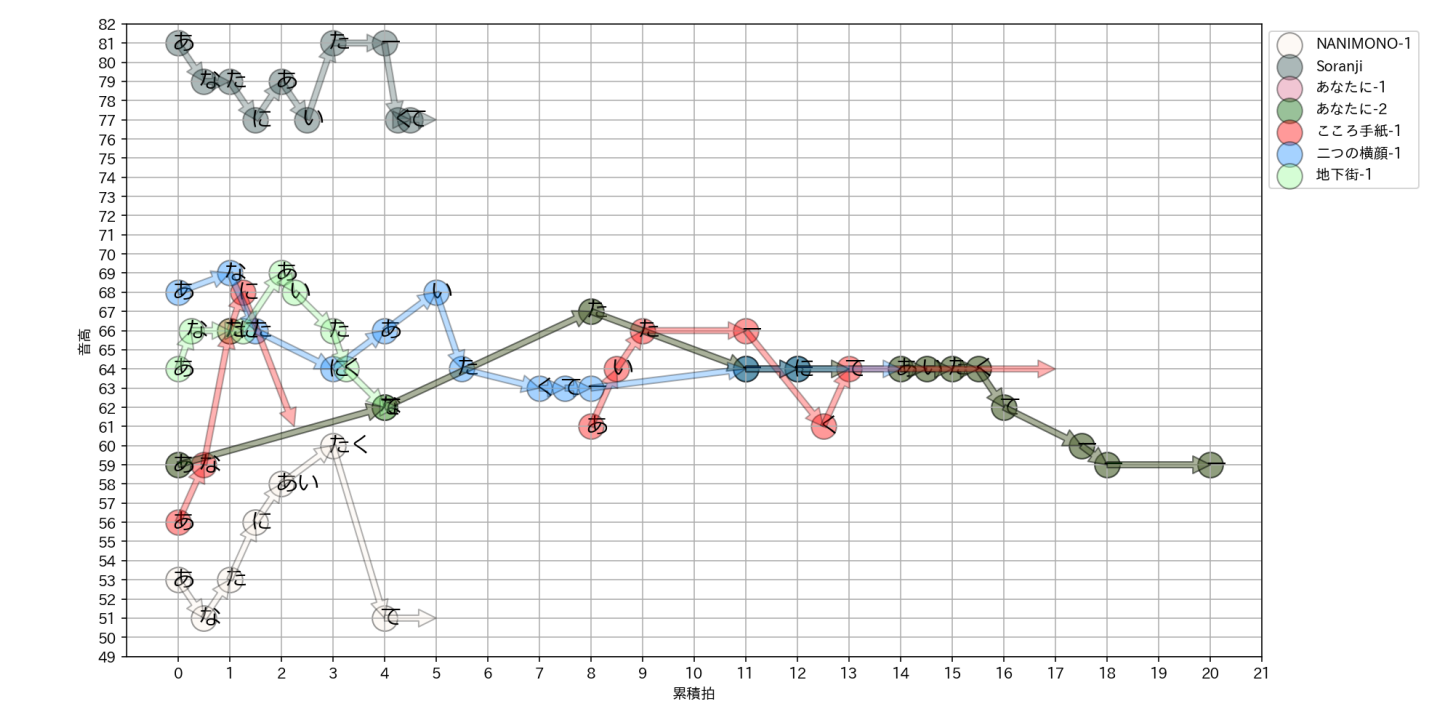
\includegraphics[width=\columnwidth]{fig/akanesann.png}
    \subcaption{プロット図}
    \label{akane}
  \end{minipage}
  \caption[先行研究でのプロット]{先行研究でのプロット\cite{sikukara}.}
  \label{system}
\end{figure*}

\begin{figure*}[t]
  \centering
  \begin{minipage}{0.49\hsize}
    \centering
    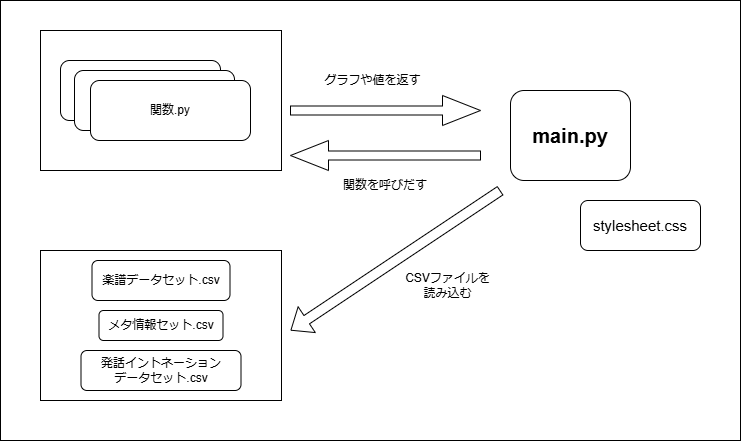
\includegraphics[width=\columnwidth]{fig/page_system.png}
    \subcaption{システム構成}
    \label{page_system}
  \end{minipage}
  \begin{minipage}{0.49\hsize}
    \centering
    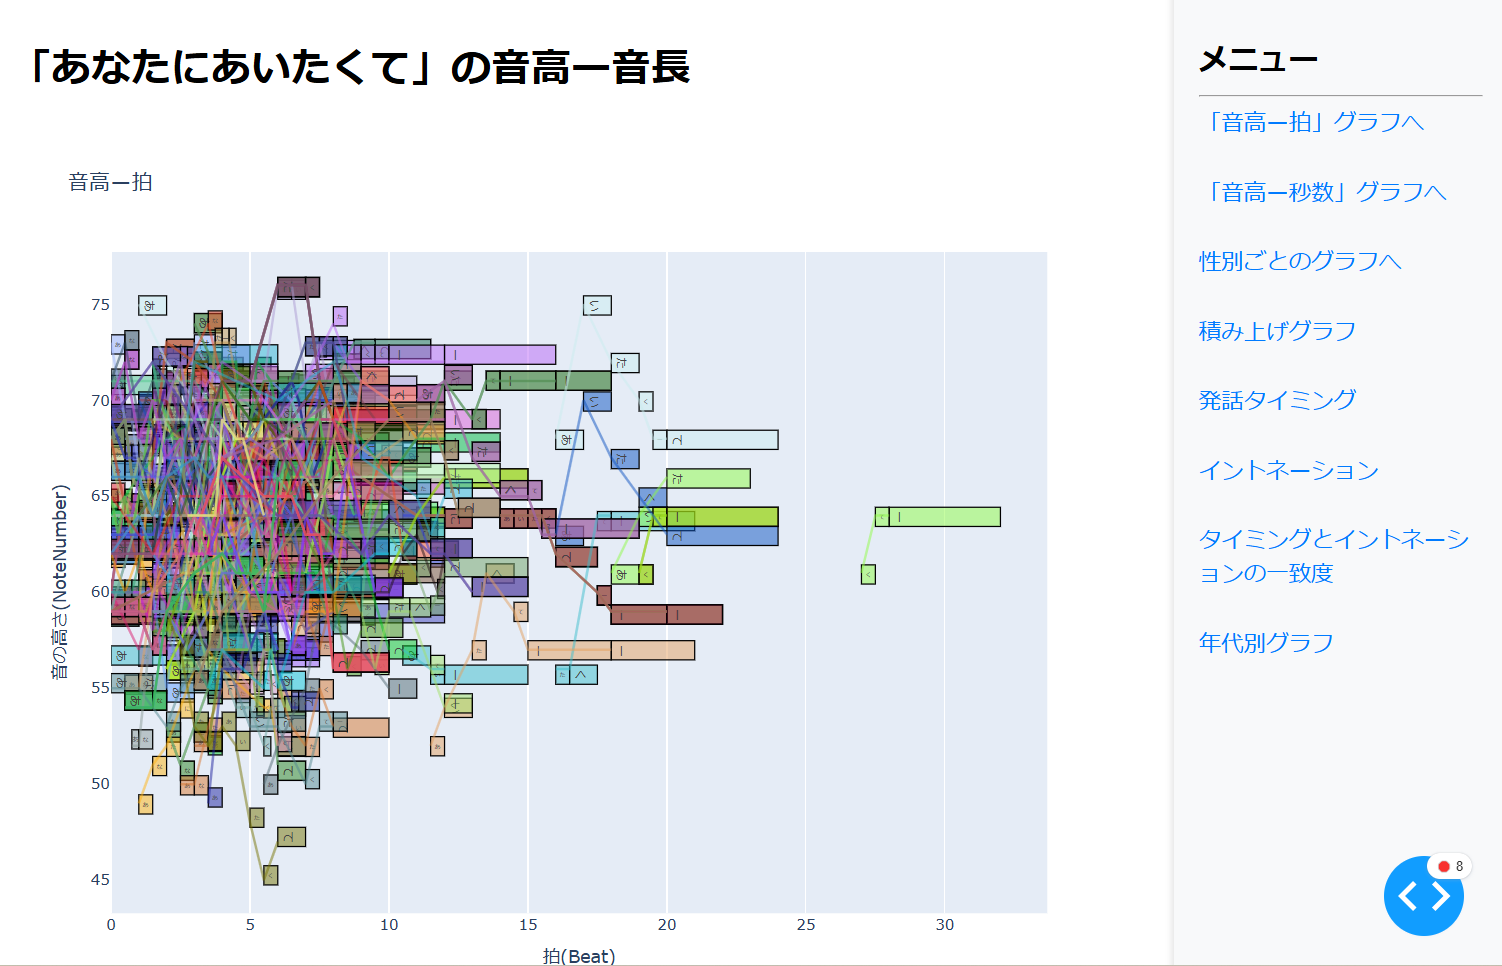
\includegraphics[width=\columnwidth]{fig/page.png}
    \subcaption{プロット図}
    \label{page}
  \end{minipage}
  \caption{本研究の分析過程}
  \label{mysystem}
\end{figure*}





%3.5.1
\subsubsection{作り方}\label{sec:3.5.1}
プログラム作成はPythonで行い，グラフの描写はPlotly\cite{plotly}，ツールの作成はDash\cite{dash}を用いて行った．\par
Plotlyを使用することにより，以下の利点が挙げられる．
\begin{itemize}
  \item マウスオーバーで情報が表示される
  \item ズームやパンが可能
  \item 表示させるデータを選ぶことができる
\end{itemize}
といった利点がある．
また，Dashの利点として，
\begin{itemize}
  \item Plotlyとの相性が良い
  \item Pythonのコードのみで動的なWebアプリを作成できる
  \item 表示させるデータを選ぶことができる
\end{itemize}
などが挙げられる．




%3.5.2
\subsubsection{先行研究との違い}

本研究の直接的な先行研究は，\ref{sec:2.3}節になる．\par
\ref{sec:2.3}節では，データのプロットを\figref{akane}のようにプロットしていた．また，見たいデータごとにプログラムを分けて制作し，ひとつづつmatplotlib\cite{matplotlib}で出力していた．先行研究でのプログラムのシステム図は\figref{kyuufairu}である．\par


本研究では，\ref{sec:3.5.1}に記載した通り，先行研究でのmatplotlibから変更し，PlotlyとDashを使用した．これにより，メインプログラムを起動するだけで各種プロットを行うことができる．また，動的なページを作成することにより，グラフを一気に見ることができる．
本研究のシステム図が\figref{page_system}，実際に作成したページの画面が\figref{page}である．
また，グラフ表示を\figref{akane}から\figref{kakudai}のように変更することにより，音の伸びがよりわかりやすくなった．



\begin{figure}[tb]
  \centering
  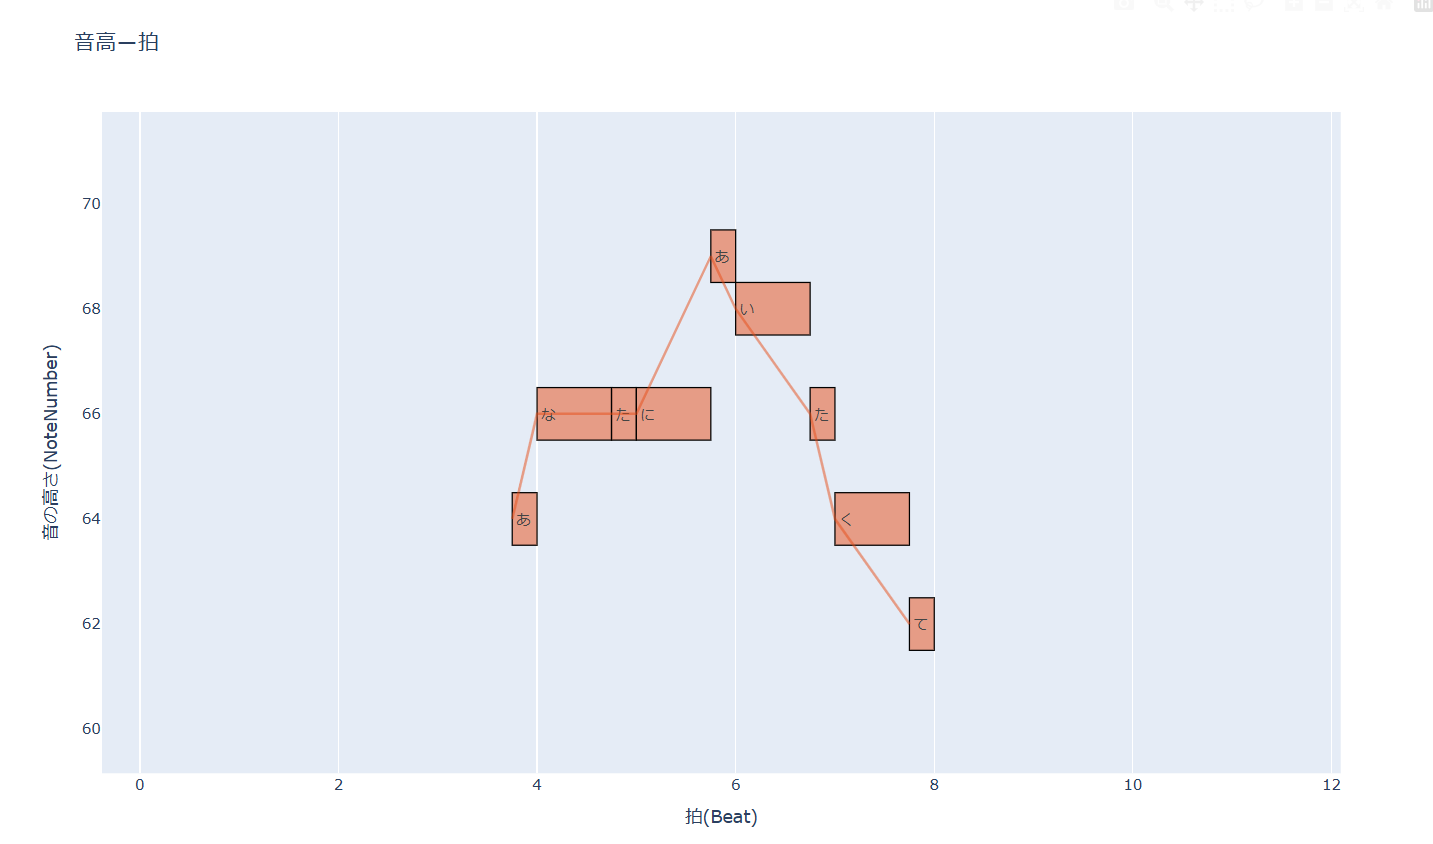
\includegraphics[width=\columnwidth]{fig/onko_haku_koma.png}
  \caption{グラフのセット（拡大）}
  \label{kakudai}
\end{figure}





\begin{figure*}[t]
  \centering
  \begin{minipage}{0.49\hsize}
    \centering
    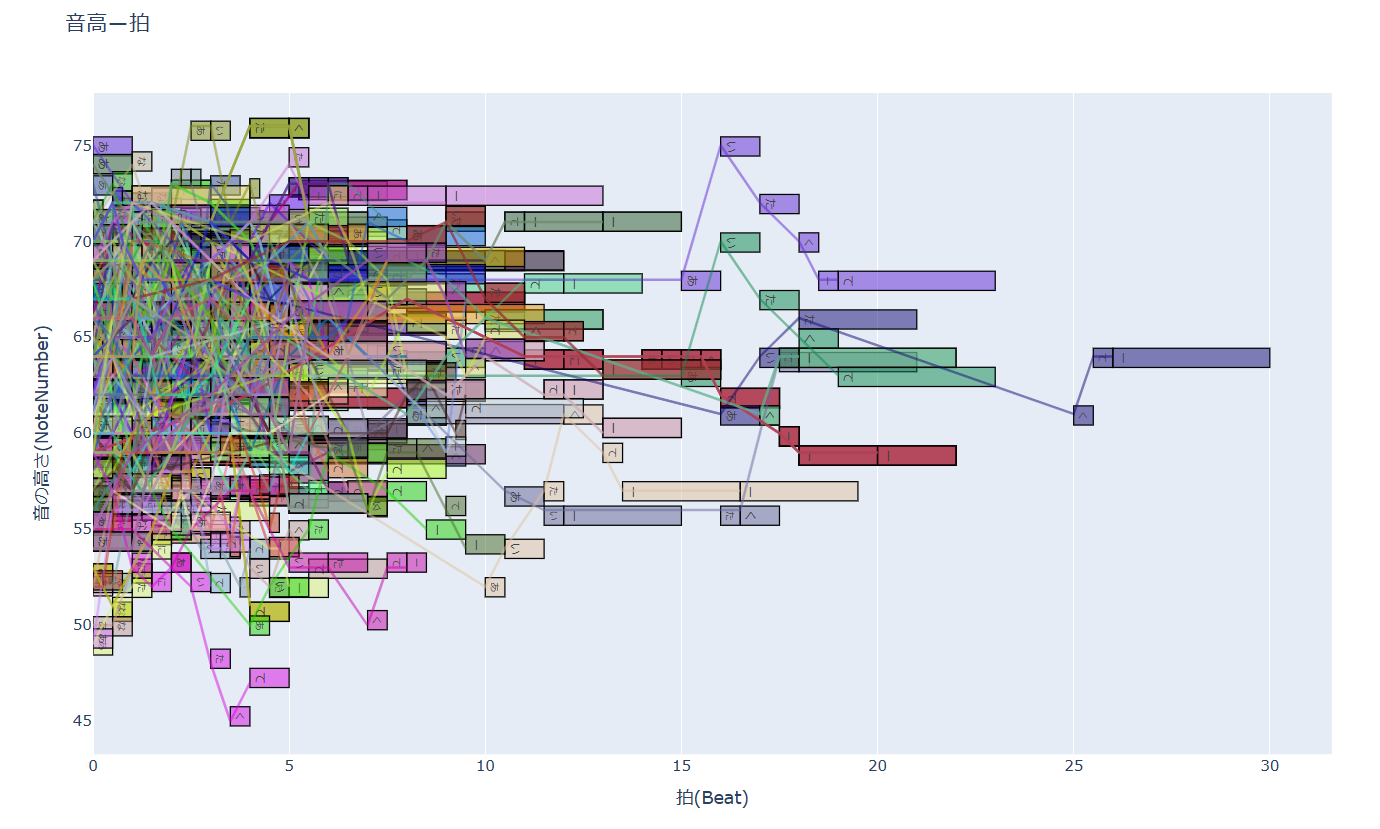
\includegraphics[width=\columnwidth]{fig/anata/onko_haku.png}
    \subcaption{“あなたにあいたくて”}
    \label{onko_haku_a}
  \end{minipage}
  \begin{minipage}{0.49\hsize}
    \centering
    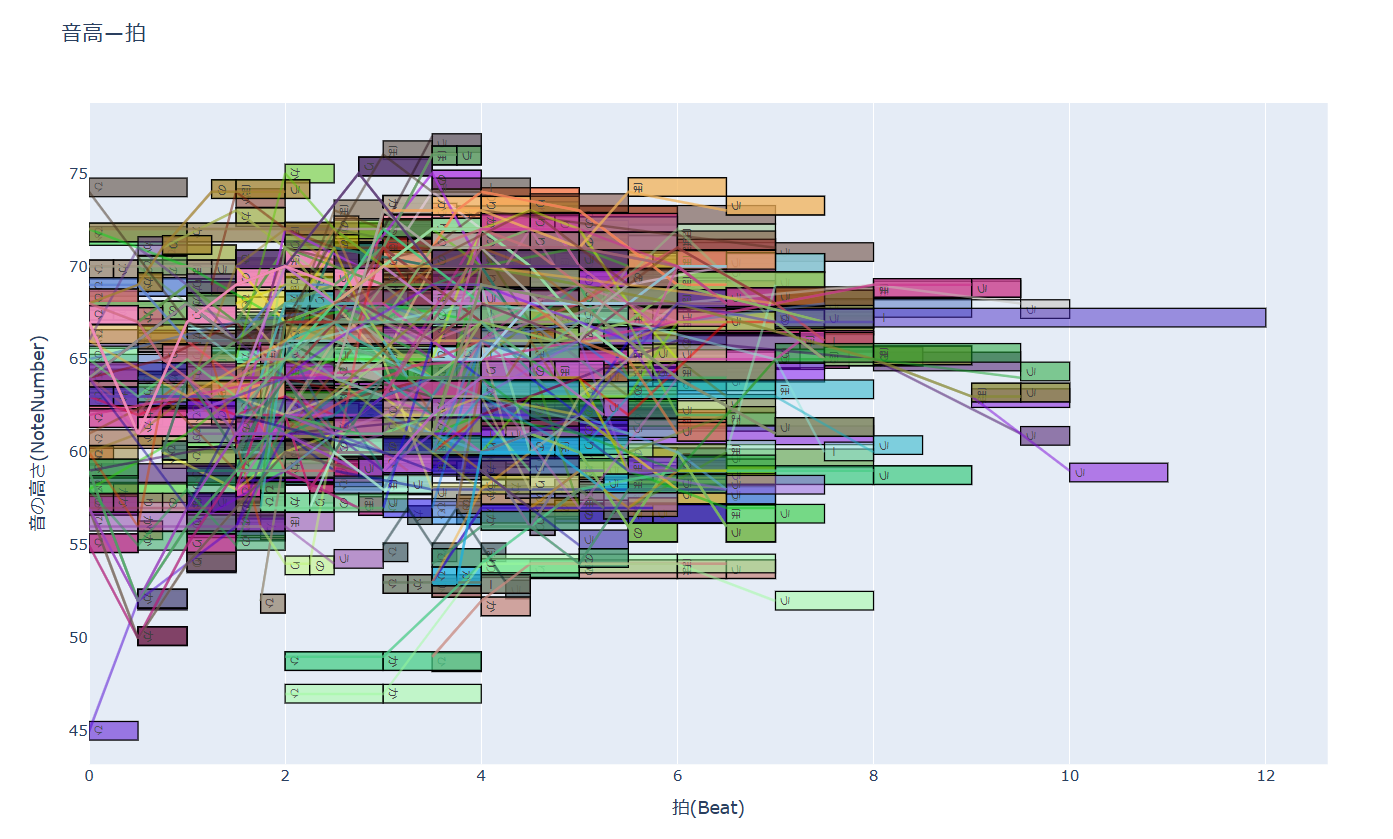
\includegraphics[width=\columnwidth]{fig/hikari/onko_haku_h.png}
    \subcaption{“ひかりのほう”}
    \label{onko_haku_h}
  \end{minipage}
  \caption{音高ー拍のプロット}
  \label{onko_haku}
\end{figure*}

\begin{figure*}[t]
  \centering
  \begin{minipage}{0.49\hsize}
    \centering
    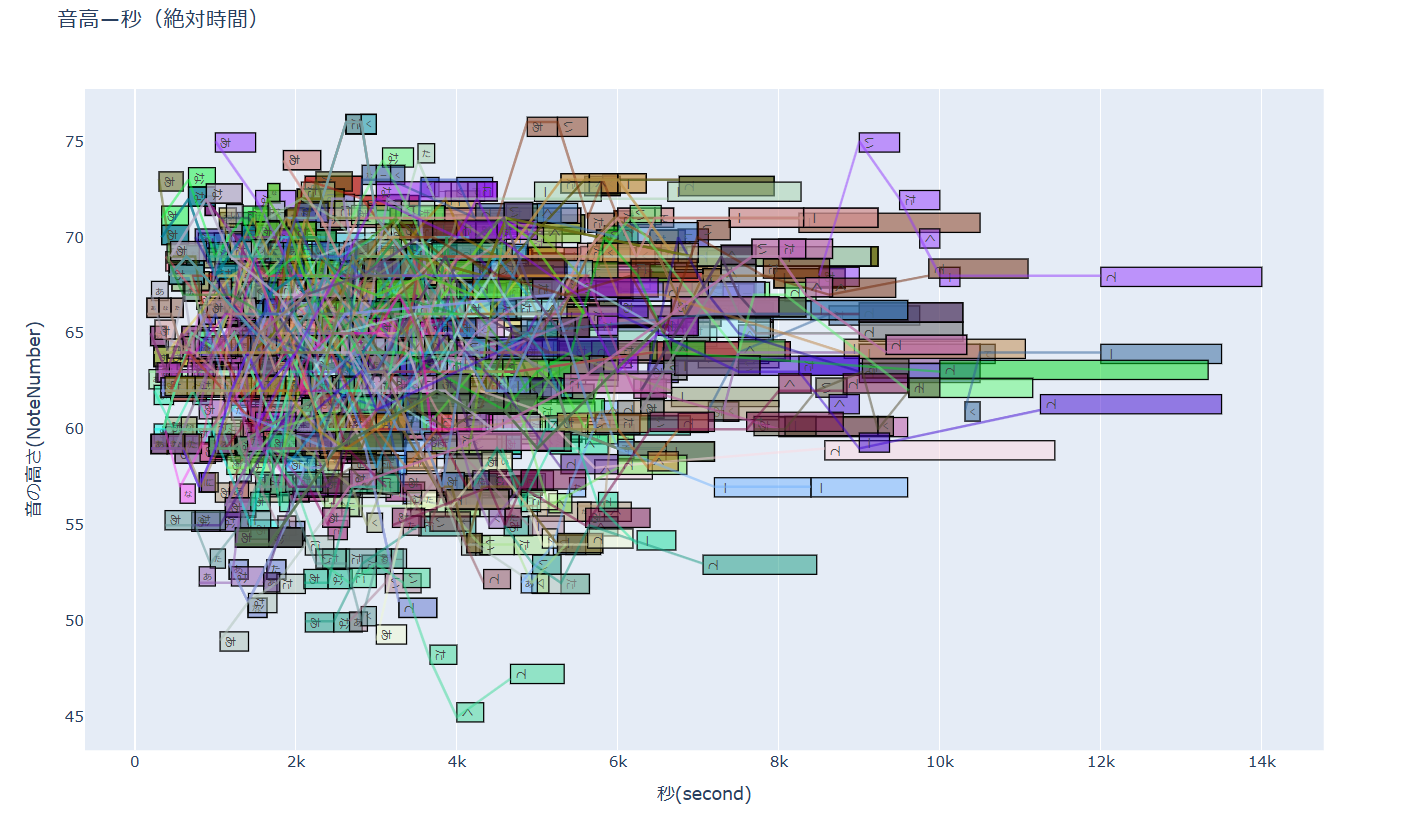
\includegraphics[width=\columnwidth]{fig/anata/onko_byou.png}
    \subcaption{“あなたにあいたくて”}
    \label{a_byou}
  \end{minipage}
  \begin{minipage}{0.49\hsize}
    \centering
    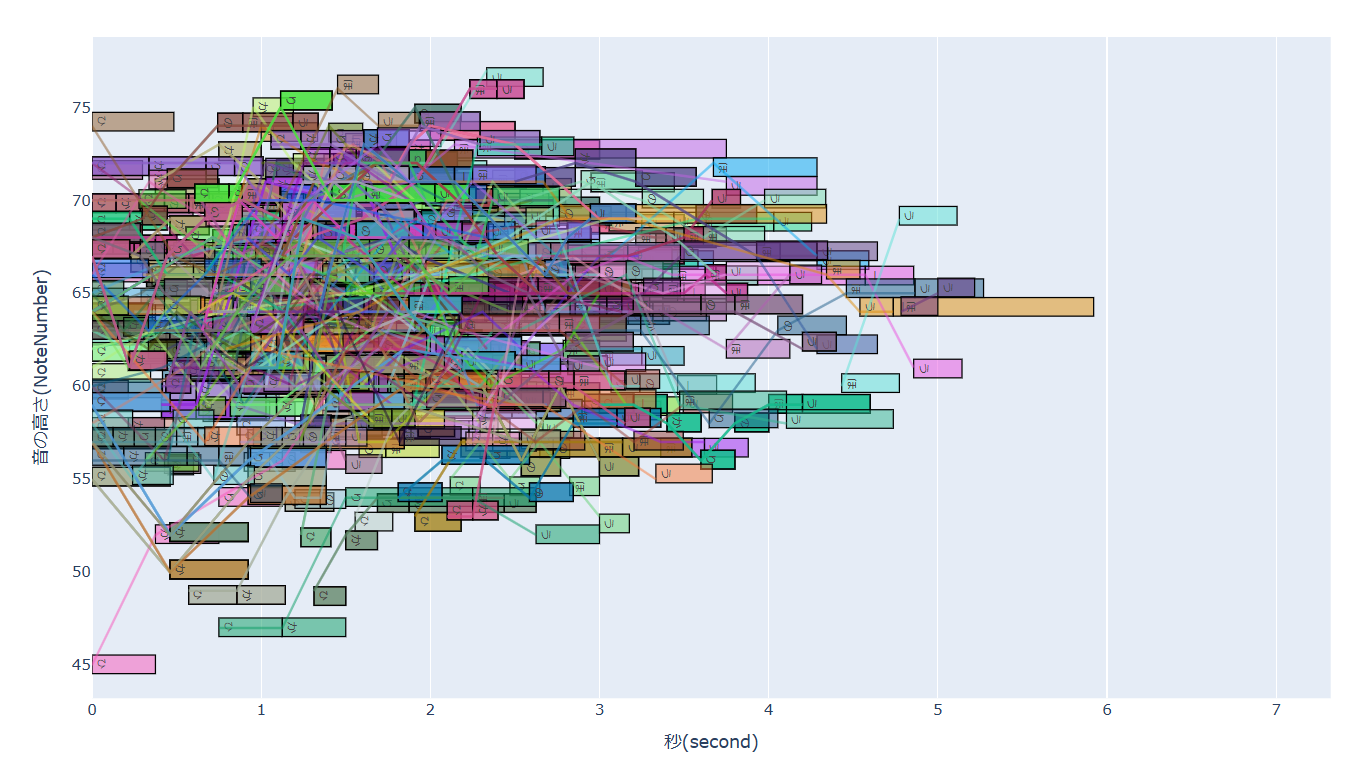
\includegraphics[width=\columnwidth]{fig/hikari/onko_byou.png}
    \subcaption{“ひかりのほう”}
    \label{h_byou}
  \end{minipage}
  \caption{音高-秒数のプロット}
  \label{byou}
\end{figure*}
\begin{figure*}[t]
  \centering
  \begin{minipage}[b]{0.62\hsize}
    \centering
    \begin{minipage}{0.49\hsize}
      \centering
      \subcaption{“あなたにあいたくて”}
      \label{a_byou_k}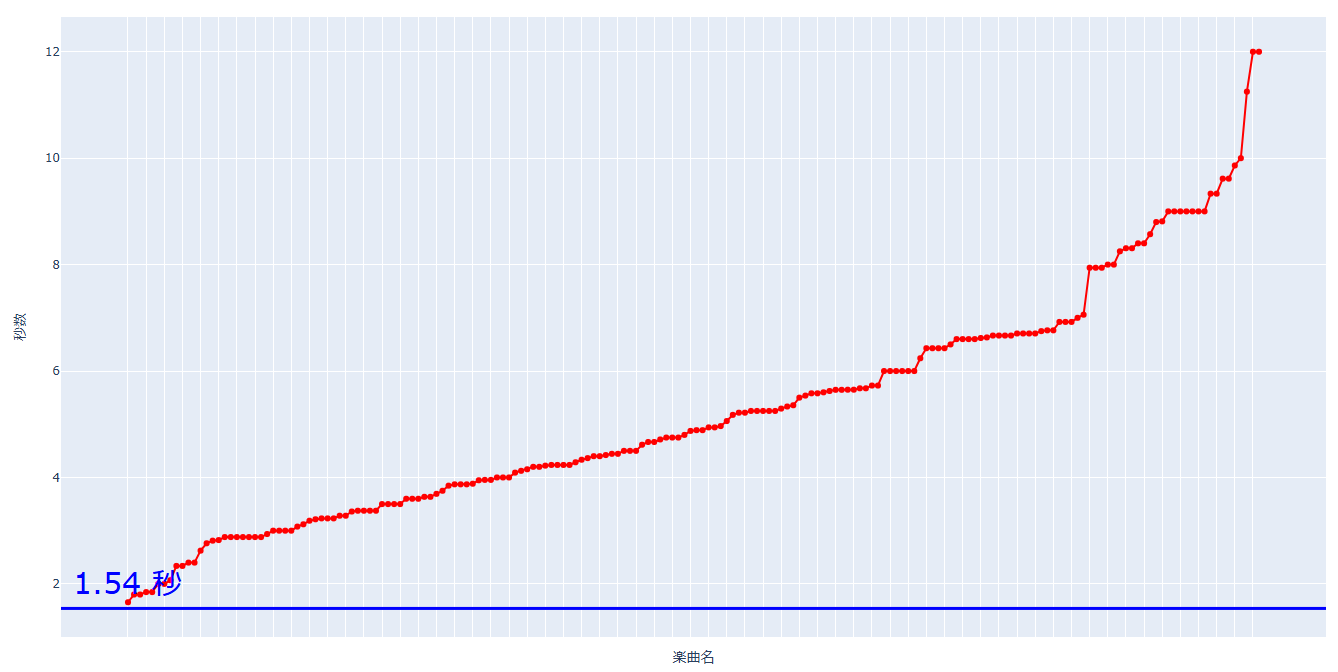
\includegraphics[width=\columnwidth]{fig/anata/byou_zentai.png}
    \end{minipage}
    \begin{minipage}{0.49\hsize}
      \centering
      \subcaption{“ひかりのほう”}
      \label{h_byou_k}
      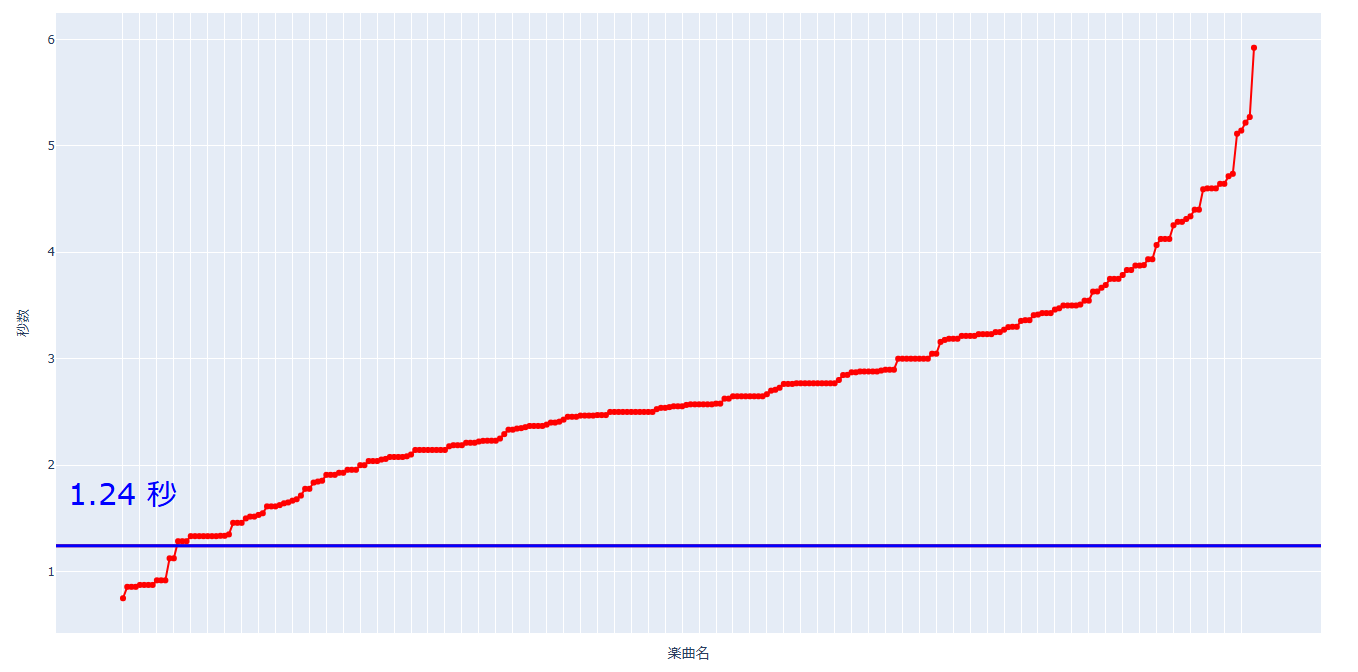
\includegraphics[width=\columnwidth]{fig/hikari/byou_zentai.png}
    \end{minipage}
    \caption{発話表現の秒数と各フレーズの秒数の比較}
    \label{kizyun_byou}
  \end{minipage}
  \begin{minipage}[b]{0.32\hsize}
    \centering
    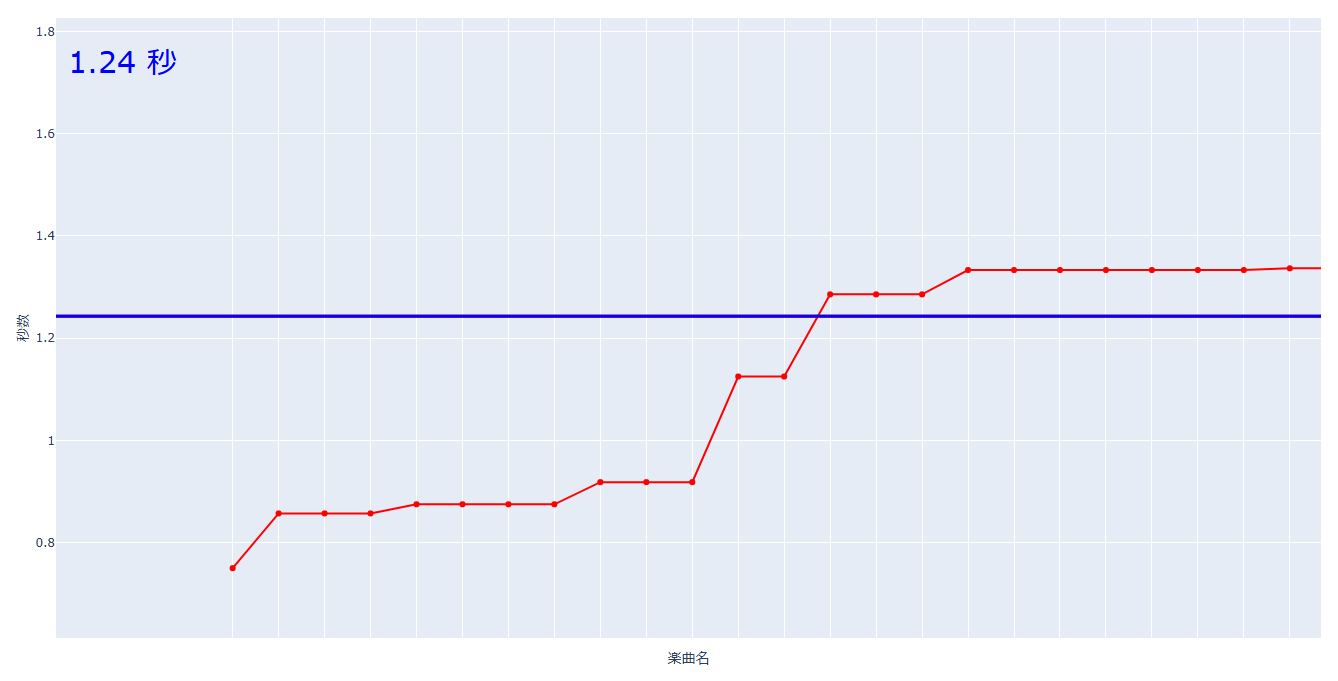
\includegraphics[width=\columnwidth]{fig/hikari/byou_koma.png}
    \caption{図13の境目付近の拡大}
    \label{b_byou_koma}
  \end{minipage}
\end{figure*}



%4
\section{結果}\label{sec:4}
これから，“あなたにあいたくて”“ひかりのほう”の2つのフレーズについて，以下の事柄に関して解析結果を出していく．
\begin{musequote}
  \begin{itemize}
    \item 音高-音長（拍）グラフ
    \item 音高-秒数グラフ
    \item 発話タイミングと歌唱タイミングの違い
    \item 発話イントネーションと歌唱イントネーションの違い
    \item 「あなたにあいたくて」における発話と歌唱の一致度
    \item 歌唱者の性別差での比較
    \item 年代別での比較
    \item 表拍・裏拍の割合
    \item 音高の分布図
  \end{itemize}
\end{musequote}

%4.1
\subsection{音高-拍のプロット}\label{sec:4.1}

x軸を歌詞の始点からオフセットを数えなおしたもの，y軸をMIDIナンバーでプロットしたのが\figref{onko_haku_a}である．\par
\textbf{“あなたにあいたくて”での結果}\par
\figref{onko_haku_a}により，拍単位だと10拍目あたりまでに音が集まっており，また，最長では30拍で歌われている楽曲があることがわかる．\par
%\begin{figure}[tb]
%  \centering
%  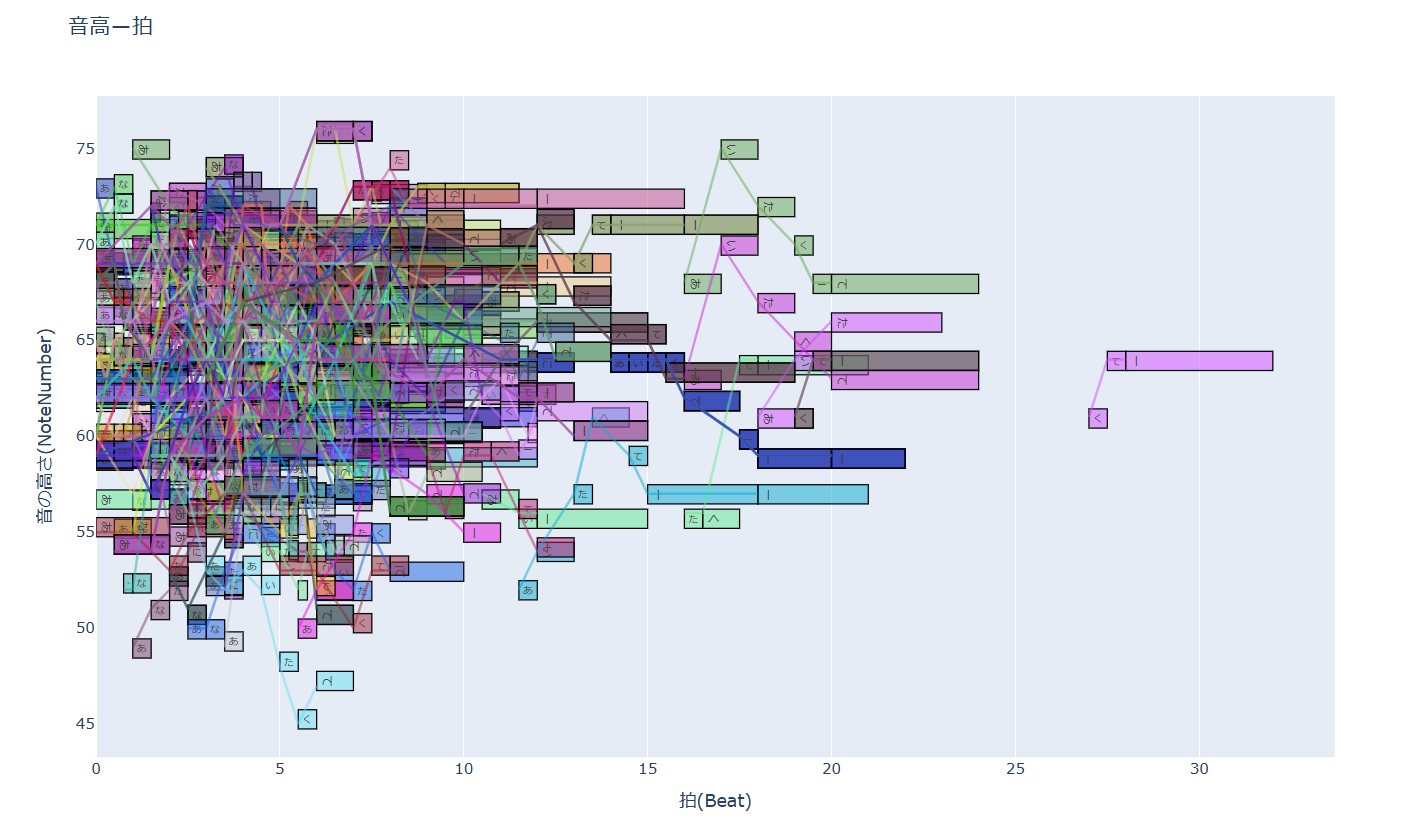
\includegraphics[width=\columnwidth]{fig/onko_haku.png}
%  \caption{音高ー拍のプロット（あ）}
%  \label{onko_haku}
%\end{figure}
\textbf{“ひかりのほう”での結果}\par
\figref{onko_haku_h}により，拍単位だと最長で10拍目までで歌い切られている．\par
%また，MIDIナンバーは45～77で，つまりA2～F5の範囲で歌われている．
%\begin{figure}[tb]
%  \centering
%  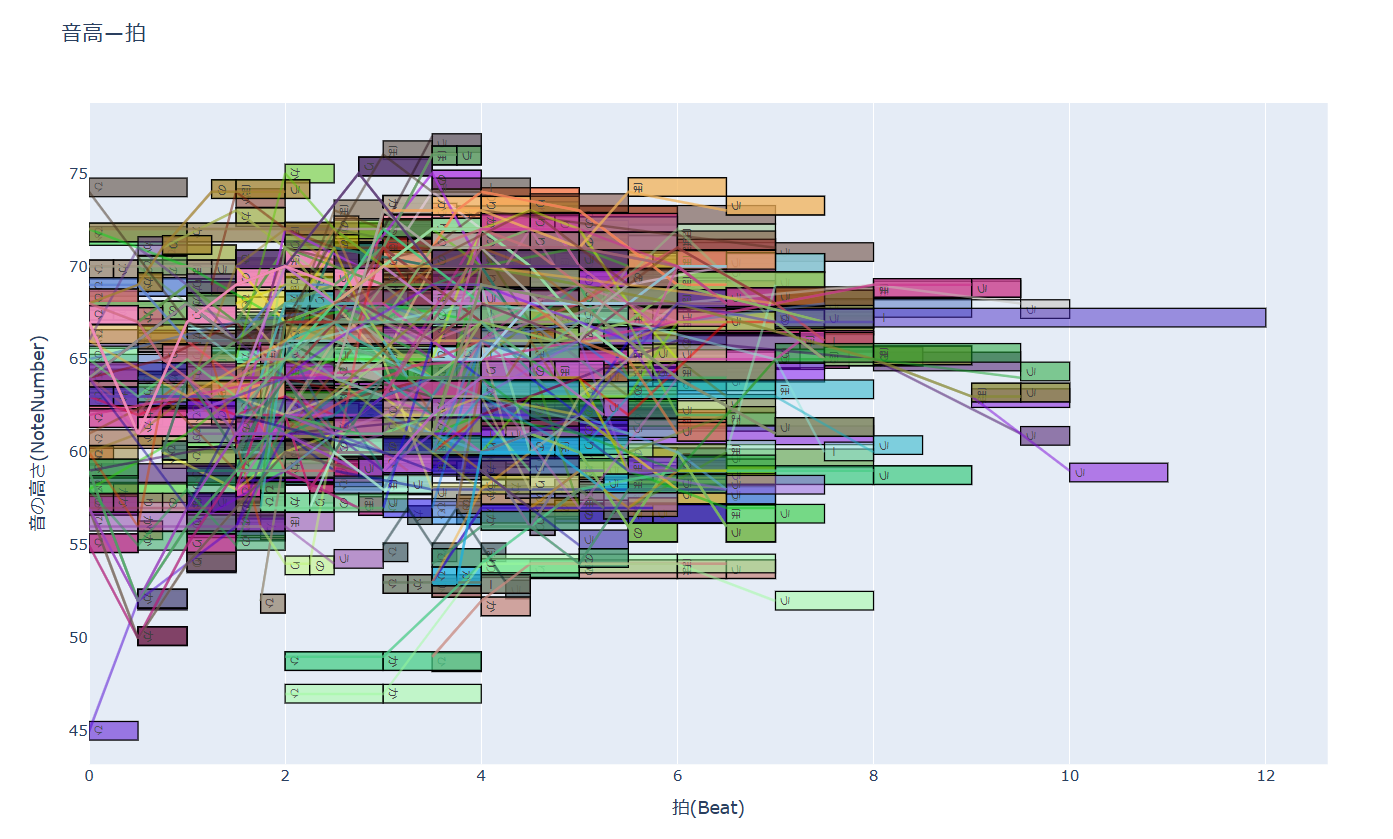
\includegraphics[width=\columnwidth]{fig/hikari/onko_haku_h.png}
%  \caption{音高ー拍のプロット（ひ）}
%  \label{onko_haku_h}
%\end{figure}


%4.2
\subsection{秒数のプロット}
%4.2.1
\subsubsection{音高-秒数のプロット}\label{4.2.1}
x軸を経過秒数，y軸をMIDIナンバーでプロットしたのが\figref{byou}である．\par

\textbf{“あなたにあいたくて”での結果}\par
\figref{onko_haku_a}では，\figref{a_byou}により，遅くとも12秒までで歌い切られていることがわかる．\par

\textbf{“ひかりのほう”での結果}\par
\figref{h_byou}より，長くても6秒までで歌い切られていることがわかる．
%4.2.2
\subsubsection{発話の経過秒との比較}
VOICEPEAKで出力した「あなたにあいたくて」「ひかりのほう」それぞれの発話表現の経過秒を基準とし，各フレーズの経過秒との違いをプロットしたのが\figref{kizyun_byou}である．



\textbf{“あなたにあいたくて”での結果}\par
\figref{a_byou_k}より，発話表現の秒数よりも早く歌い切られているフレーズはなく，全てのフレーズにおいて発話表現よりも遅く歌い切られていることがわかる．%また，\red{（同楽曲のフレーズが重複しているとはいえ）一次関数的に伸びていることが何か言えそう}


\begin{figure*}[t]
  \centering
  \begin{minipage}{0.49\hsize}
    \centering
    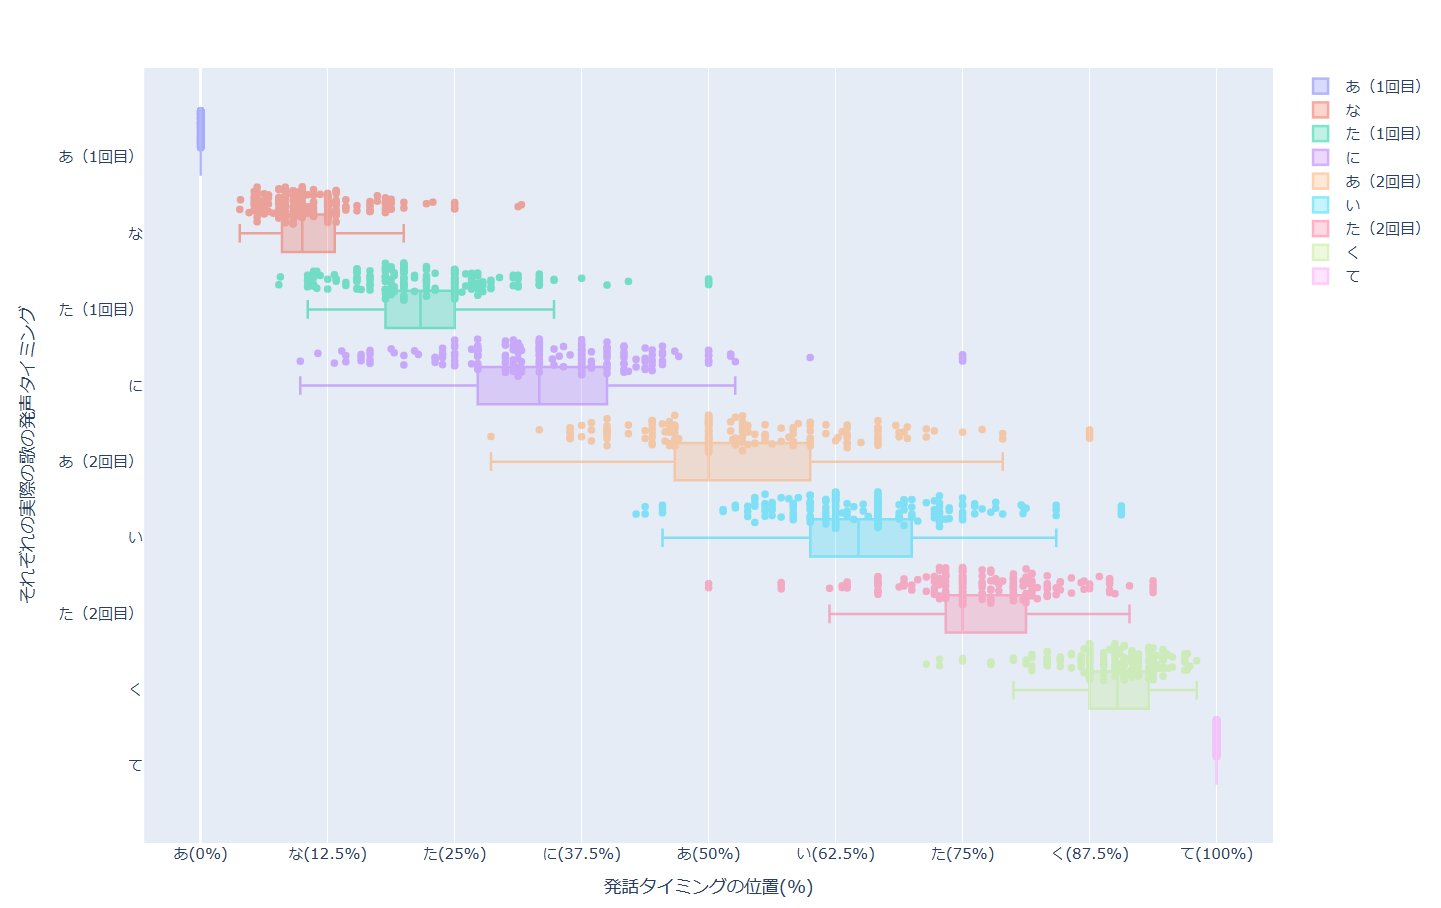
\includegraphics[width=\columnwidth]{fig/anata/hakohige_tai.png}
    \subcaption{“あなたにあいたくて”}
    \label{a_ha_tai}
  \end{minipage}
  \begin{minipage}{0.49\hsize}
    \centering
    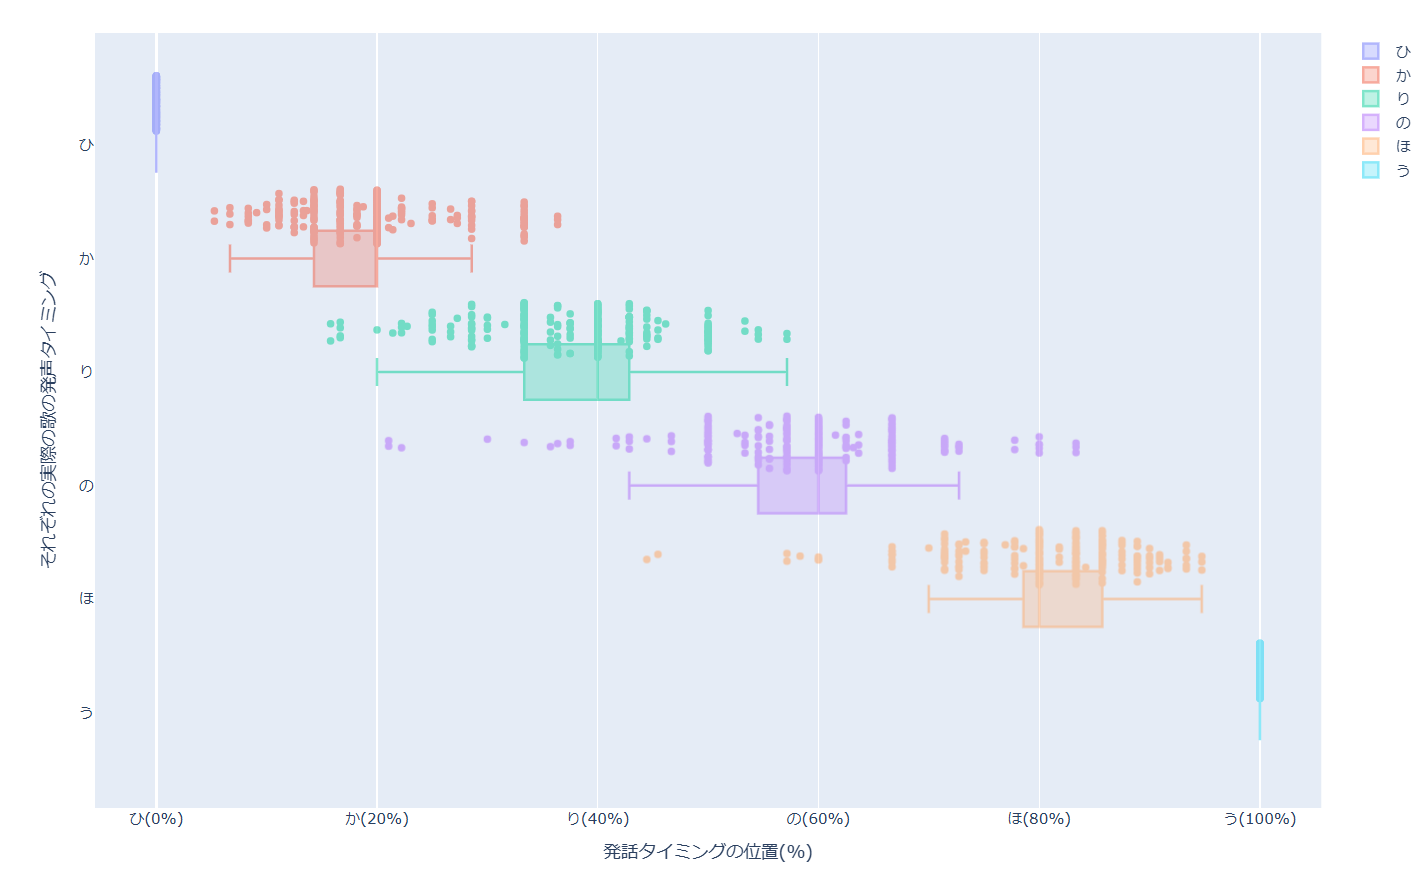
\includegraphics[width=\columnwidth]{fig/hikari/hakohige_tai.png}
    \subcaption{“ひかりのほう”}
    \label{h_ha_tai}
  \end{minipage}
  \caption{発話タイミングと歌のずれ}
  \label{ha_tai}
\end{figure*}
\begin{figure*}[t]
  \centering
  \begin{minipage}{0.49\hsize}
    \centering
    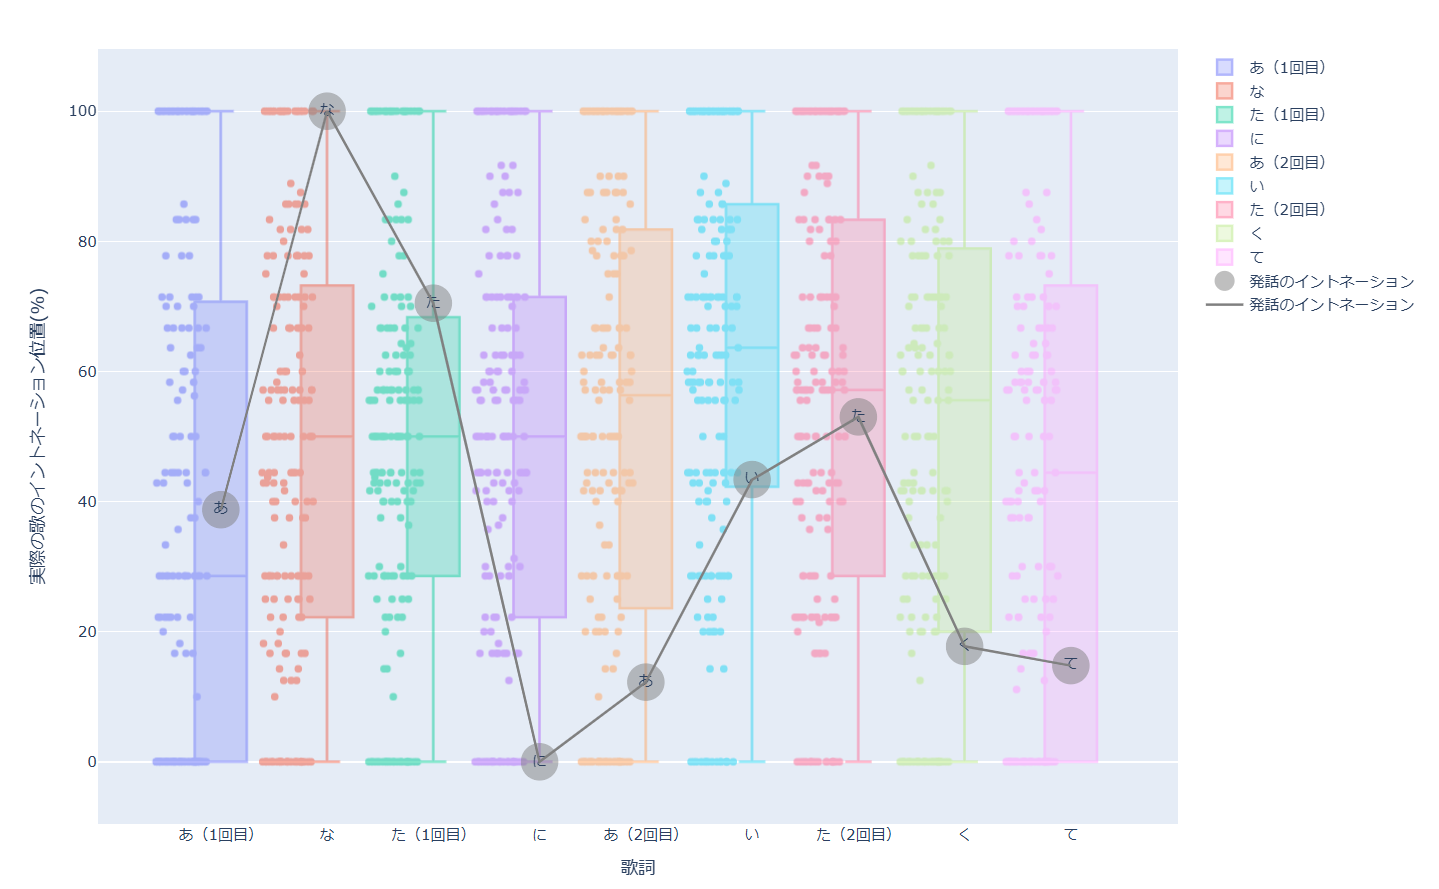
\includegraphics[width=\columnwidth]{fig/anata/hakohige_into.png}
    \subcaption{“あなたにあいたくて”}
    \label{a_ha_into}
  \end{minipage}
  \begin{minipage}{0.49\hsize}
    \centering
    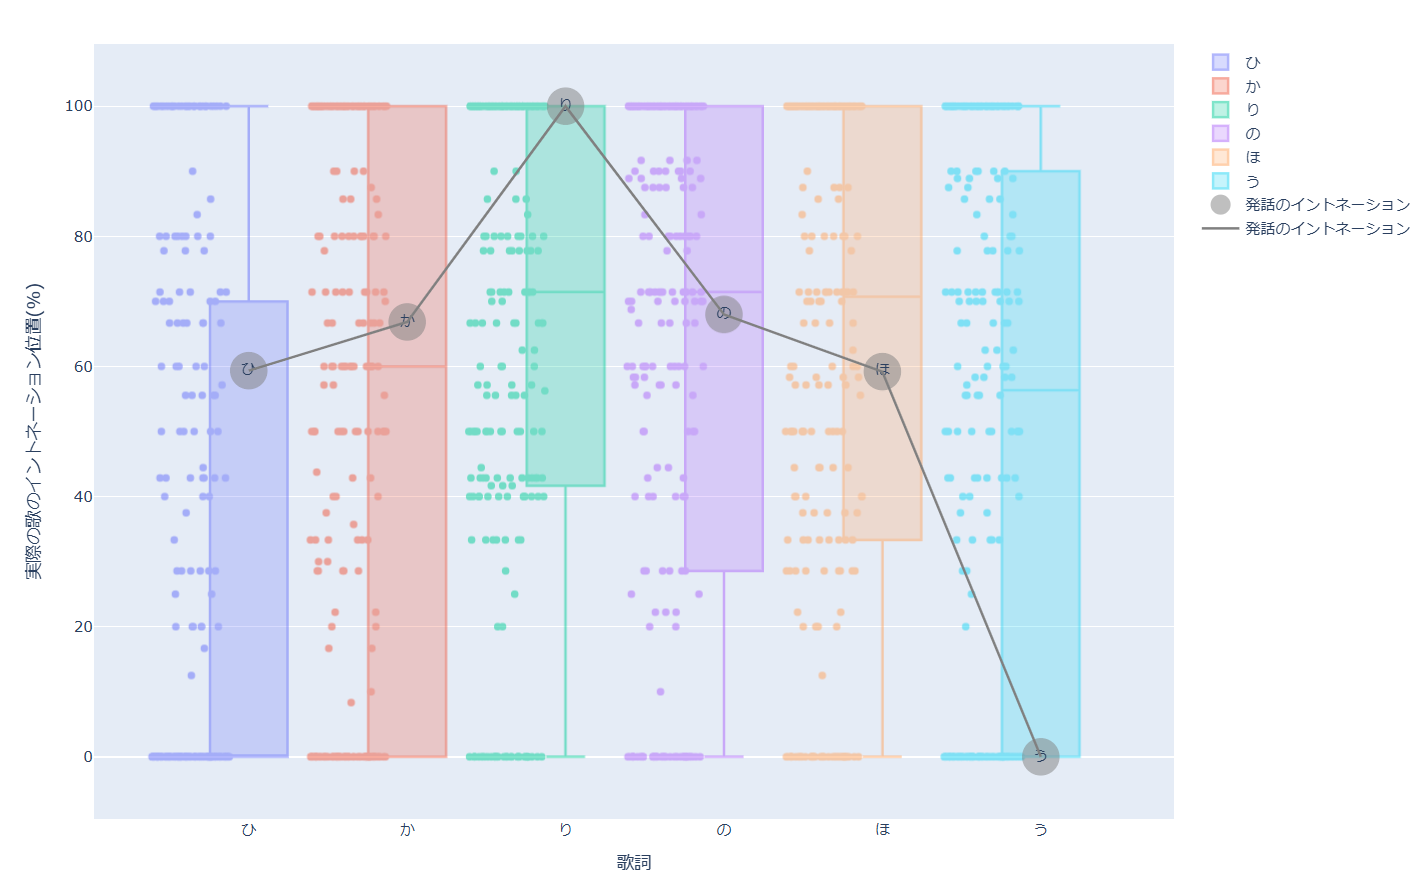
\includegraphics[width=\columnwidth]{fig/hikari/hakohige_into.png}
    \subcaption{“ひかりのほう”}
    \label{h_ha_into}
  \end{minipage}
  \caption{発話イントネーションと歌のずれ}
  \label{ha_into}
\end{figure*}
\begin{figure*}[t]
  \centering
  \begin{minipage}{0.49\hsize}
    \centering
    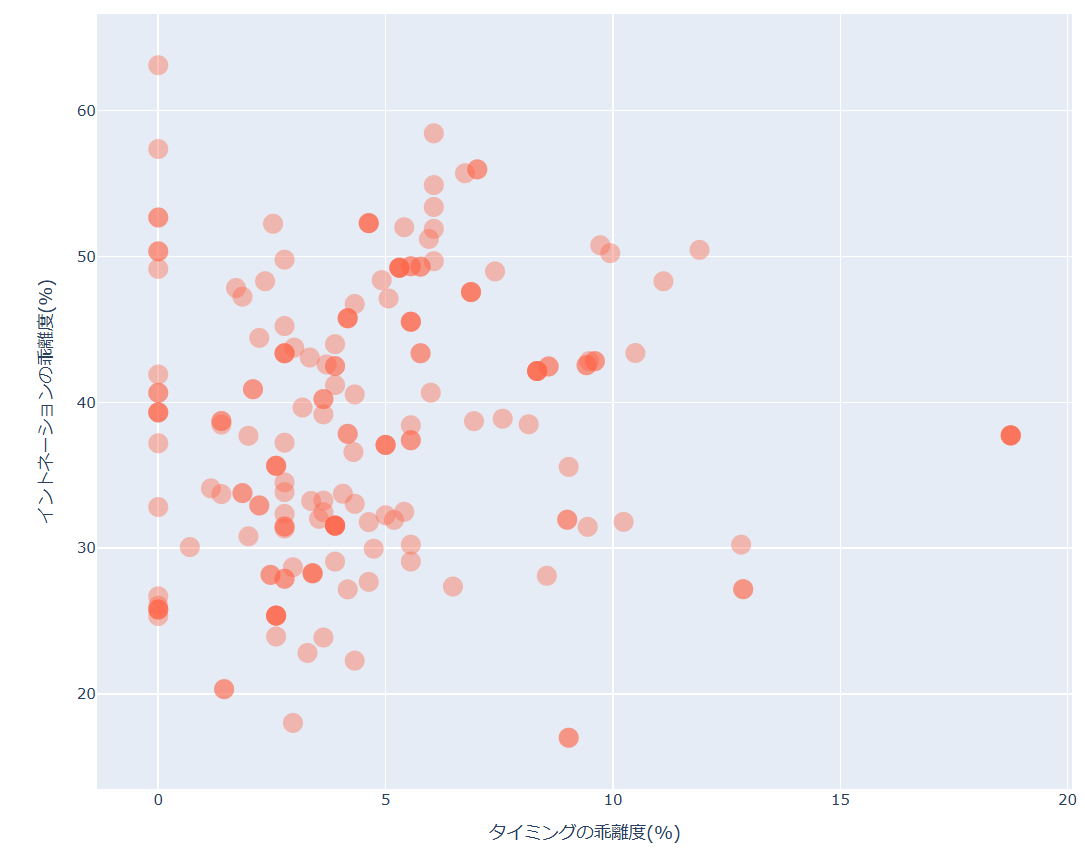
\includegraphics[width=\columnwidth]{fig/anata/bunpu.png}
    \subcaption{“あなたにあいたくて”}
    \label{a_bunpu}
  \end{minipage}
  \begin{minipage}{0.49\hsize}
    \centering
    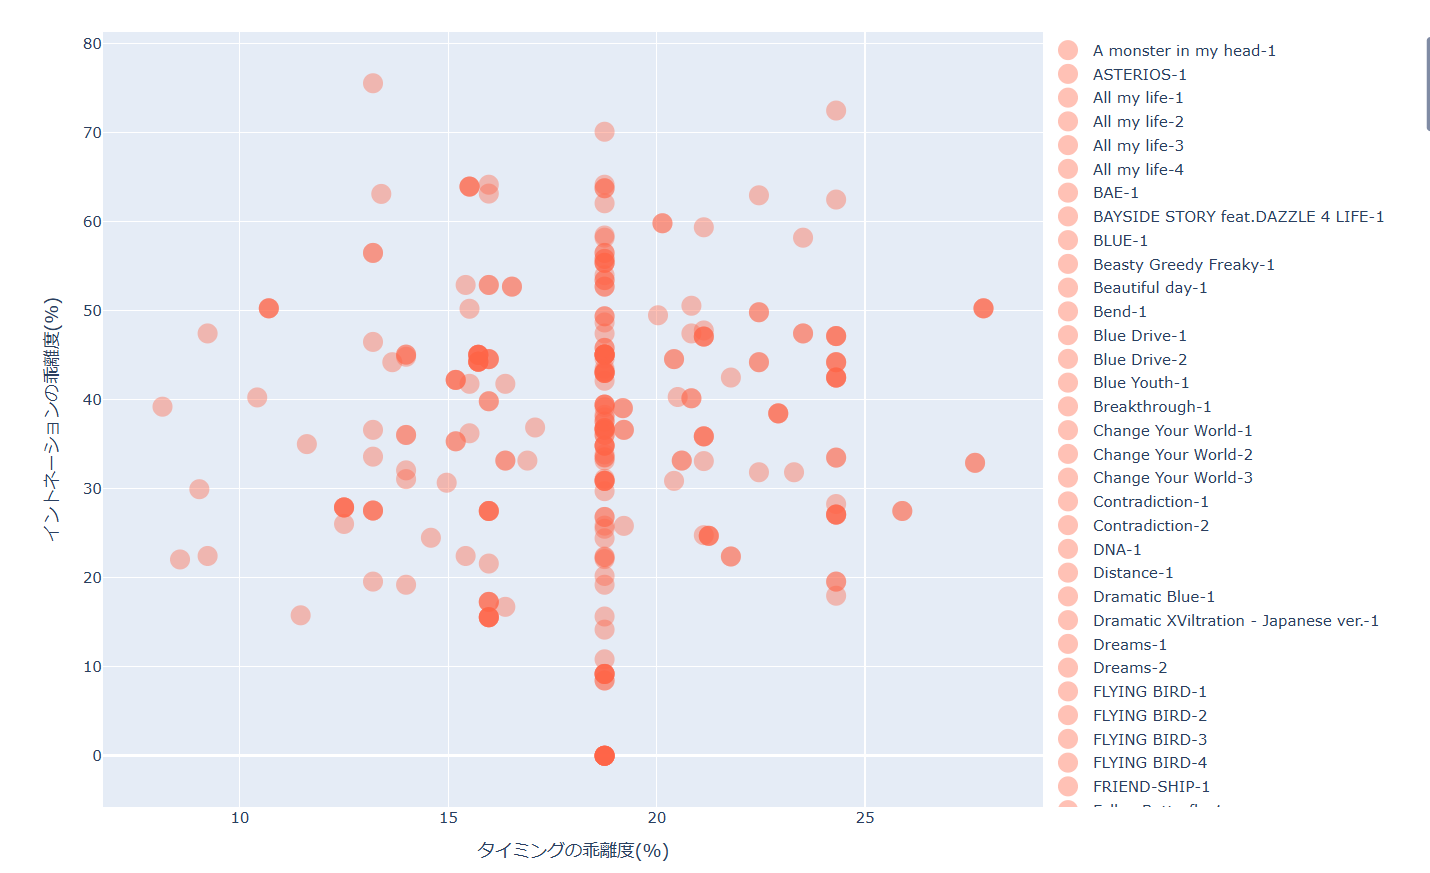
\includegraphics[width=\columnwidth]{fig/hikari/bunpu.png}
    \subcaption{“ひかりのほう”}
    \label{h_bunpu}
  \end{minipage}
  \caption{タイミングとイントネーションのずれ}
  \label{bunpu}
\end{figure*}





\textbf{“ひかりのほう”での結果}\par
\figref{h_byou_k}より，ほぼ全てのフレーズにおいて発話表現よりも遅く歌い切られているが，一部のフレーズは発話表現よりも早くに歌い切られていることがわかる．\figref{b_byou_koma}はその地点を拡大したものである．\figref{b_byou_koma}より，早く歌い切られているフレーズは13フレーズあり，そのうち11フレーズは1秒未満であることがわかる．






%4.3
\subsection{タイミングとイントネーション}
%4.3.1
\subsubsection{発話タイミング}\label{sec:4.3.1}
“あなたにあいたくて”“ひかりのほう”において，発話タイミングと歌唱タイミングとのずれを表したのが\figref{ha_tai}である．\par
各フレーズのタイミングの最初と最後を0\%と100\%とし，その間に歌われる単音がどこにいるかをパーセントに変換した．\par
%例えば，「あなたにあいたくて」の場合だと最初の“あ”を0\%，“て”を100\%とし，間にある“なたにあいたく”がそれぞれ何パーセントの位置にあるかを算出した．\par
\figref{a_ha_tai}，\figref{h_ha_tai}は，それを箱ひげ図にプロットしたものである．\par


\textbf{“あなたにあいたくて”での結果}\par
\figref{a_ha_tai}により，「あ（2回目）」と「た（2回目）」において，中央値と発話タイミングが一致していることがわかる．また，「た（1回目）」において，第一四分位数と発話タイミングが一致しているため，75\%の楽曲は発話タイミングと同じか早く発音されていることがわかる．また，「く」において，第三四分位数と発話タイミングが一致しているため，75\%の楽曲は発話タイミングと同じか遅く発音されていることがわかる．また，「に」と「あ（2回目）」において，ひげがかなり長いことから，広い範囲の音が使われていることがわかる．
%\begin{figure}[tb]
%  \centering
%  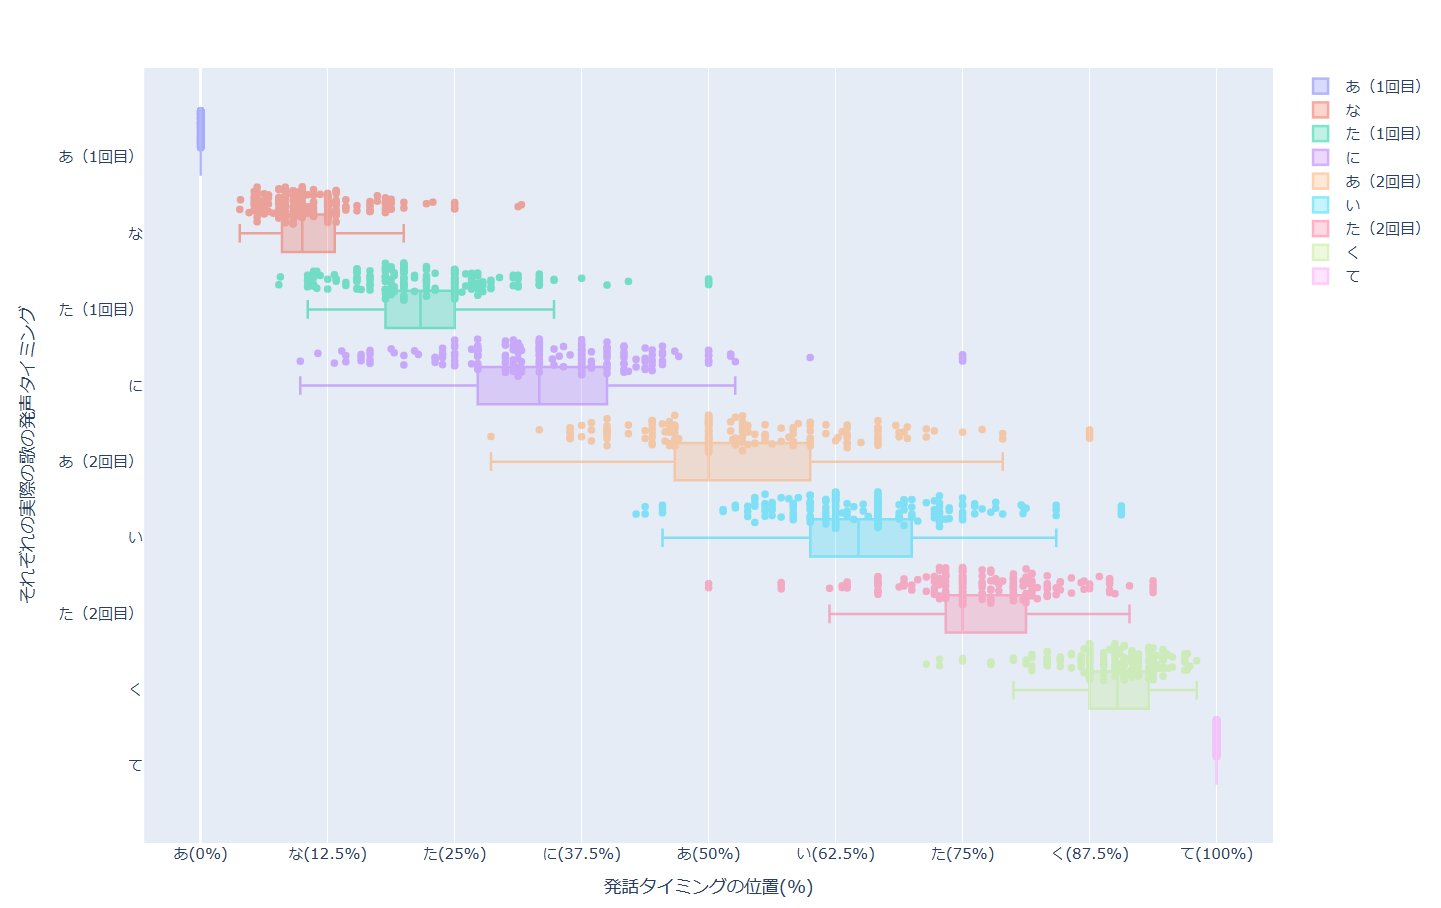
\includegraphics[width=\columnwidth]{fig/anata/hakohige_tai.png}
%  \caption{発話タイミングと歌のずれ（あ）}
%  \label{a_ha_tai}
%\end{figure}

\textbf{“ひかりのほう”での結果}\par
%“ひかりのほう”において，発話タイミングと歌唱タイミングとのずれを表したのが\figref{h_ha_tai}である．\par
\figref{h_ha_tai}により，“ひかりのほう”は全て単音において，中央値とタイミングが一致していることがわかる．また，“か”において，第三四分位数が中央値および発話タイミングと一致していることから，75\%の楽曲は発話タイミングと同じか早く発音されており，その中でも50\%から75\%に分布している，つまり25\%の楽曲は発話タイミングと一致して発音されていることがわかる．\par
%\begin{figure}[tb]
%  \centering
%  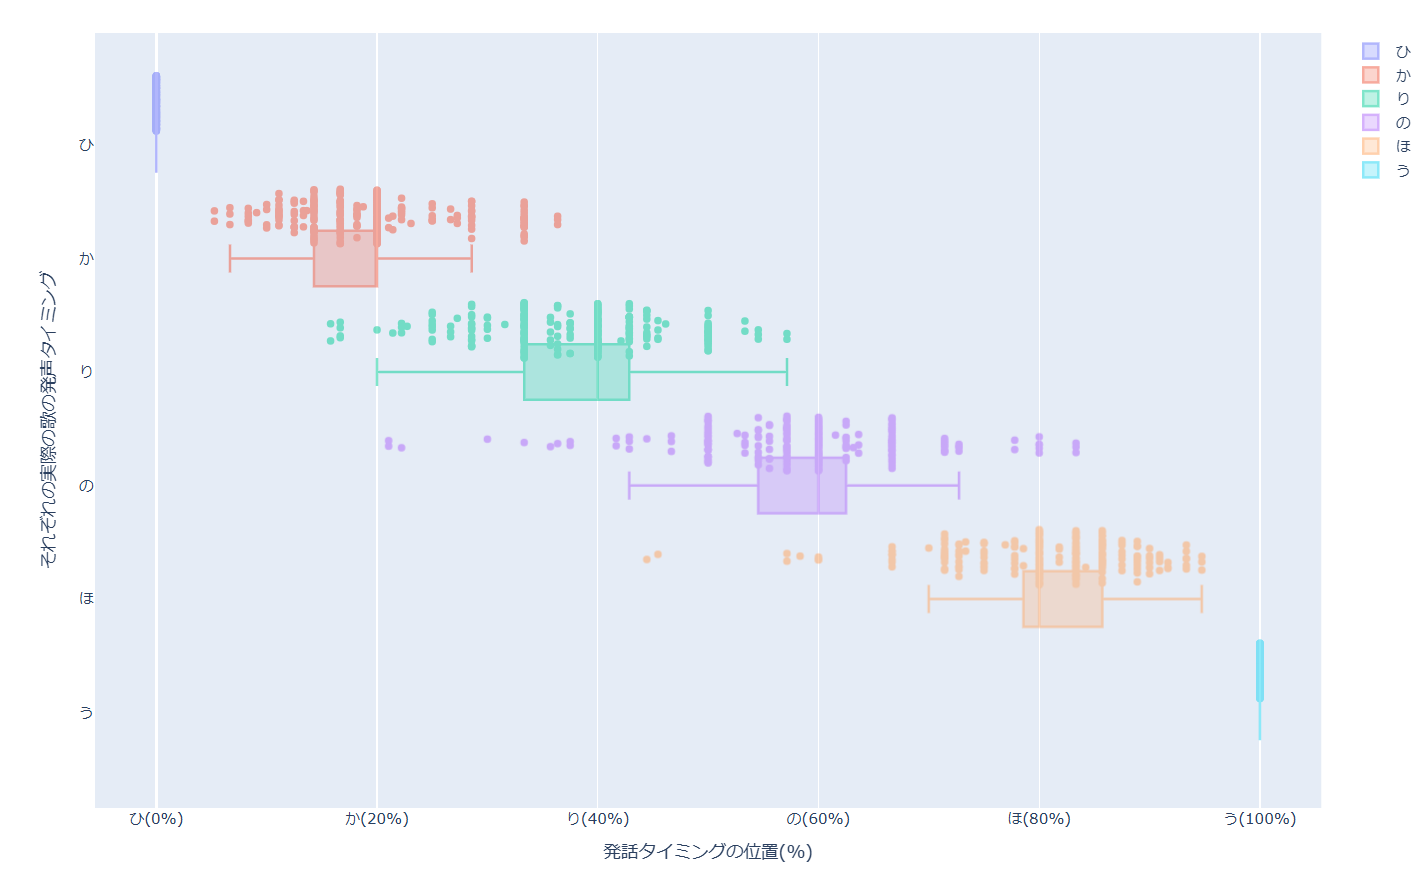
\includegraphics[width=\columnwidth]{fig/hikari/hakohige_tai.png}
%  \caption{発話タイミングと歌のずれ（ひ）}
%  \label{h_ha_tai}
%\end{figure}

%4.3.2
\subsubsection{イントネーション}\label{sec:4.3.2}
“あなたにあいたくて”“ひかりのほう”において，発話イントネーションと歌とのずれを表したのが\figref{ha_into}である．
これは，\ref{sec:4.3.1}節のように，各フレーズの最低音と最高音を0\%，100\%とし，その間の音が相対的にどの位置にいるのかをパーセントに変換した．\par
\figref{a_ha_into}，\figref{h_ha_into}は，それらを箱ひげ図にプロットしたものである．また，\ref{sec:3.4.2}節で取得した発話イントネーションのパーセントもプロットすることにより，発話イントネーションとの差がわかりやすくなっている．\par

\textbf{“あなたにあいたくて”での結果}\par
\figref{a_ha_into}により，「あ（1回目）」と「あ（2回目）」，「て」において，箱の大きさが大きいことから，ばらつきが大きいことがわかる．「あ（1回目）」と「て」において，第三四分位数が0\%の位置にあることから，各単音の最低でも4分の1がフレーズ内の最も低い音で歌われていることがわかる．\par
%\begin{figure}[tb]
%  \centering
%  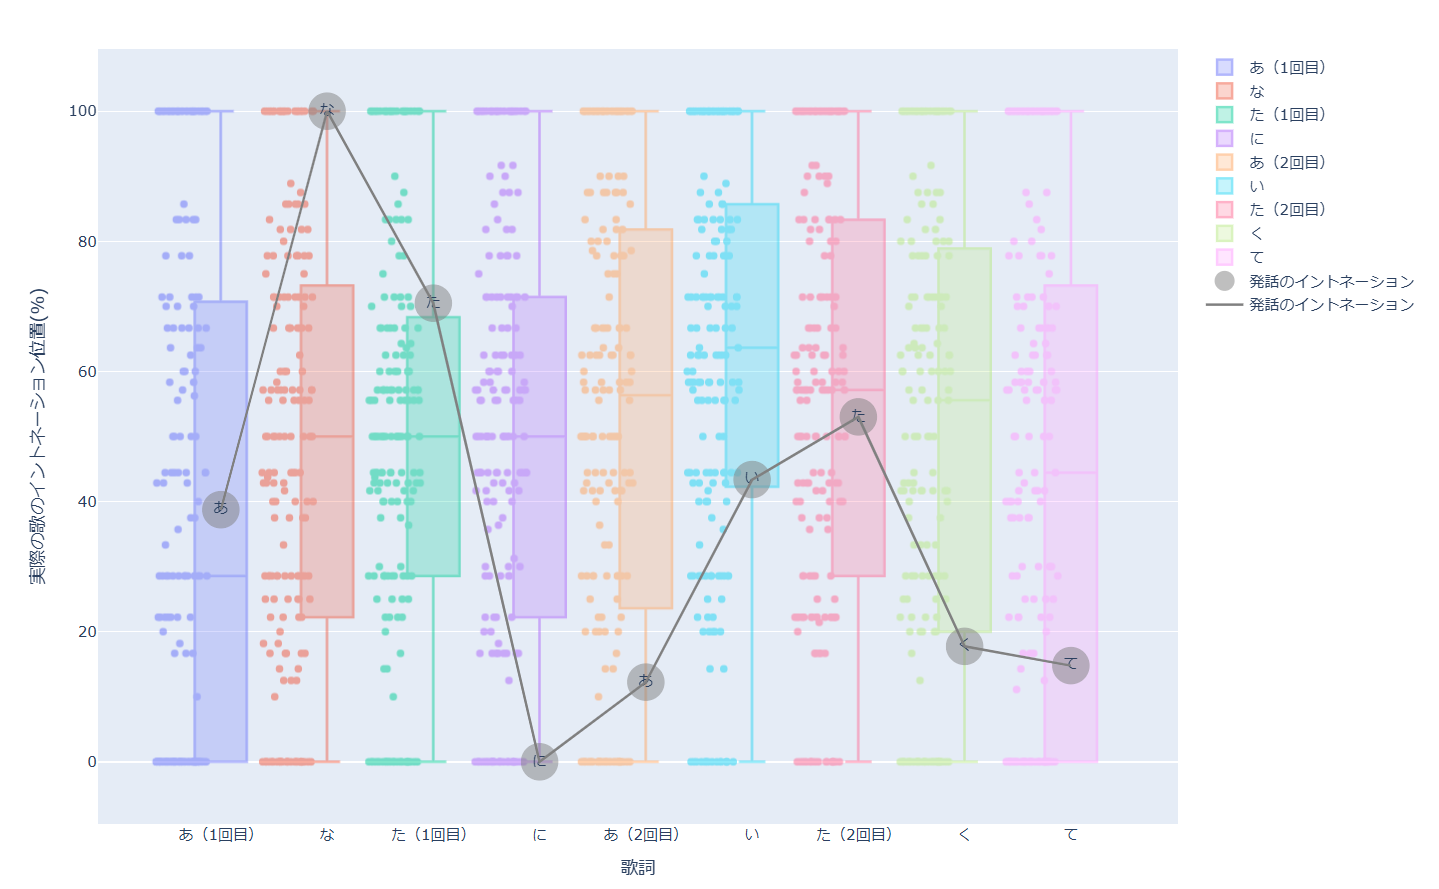
\includegraphics[width=\columnwidth]{fig/anata/hakohige_into.png}
%  \caption{発話イントネーションと歌のずれ（あ）}
%  \label{a_ha_into}
%\end{figure}

\textbf{“ひかりのほう”での結果}\par
\figref{h_ha_into}により，“ひ”においては，中央値から最小値が0にあることから，半分以上の楽曲が“ひ”を最も低く歌っていることがわかる．また，“か”“り”“の”“ほ”において，最大値および第一四分位数が100にあることから，各単音の最低でも4分の1がフレーズ内で最も高い音で歌われていることがわかる．\par
また，“か”と“う”において，最小値および第三四分位数が0の位置にあることから，各単音の最低でも4分の1がフレーズ内の最も低い音で歌われていることがわかる．\par
%\begin{figure}[tb]
%  \centering
%  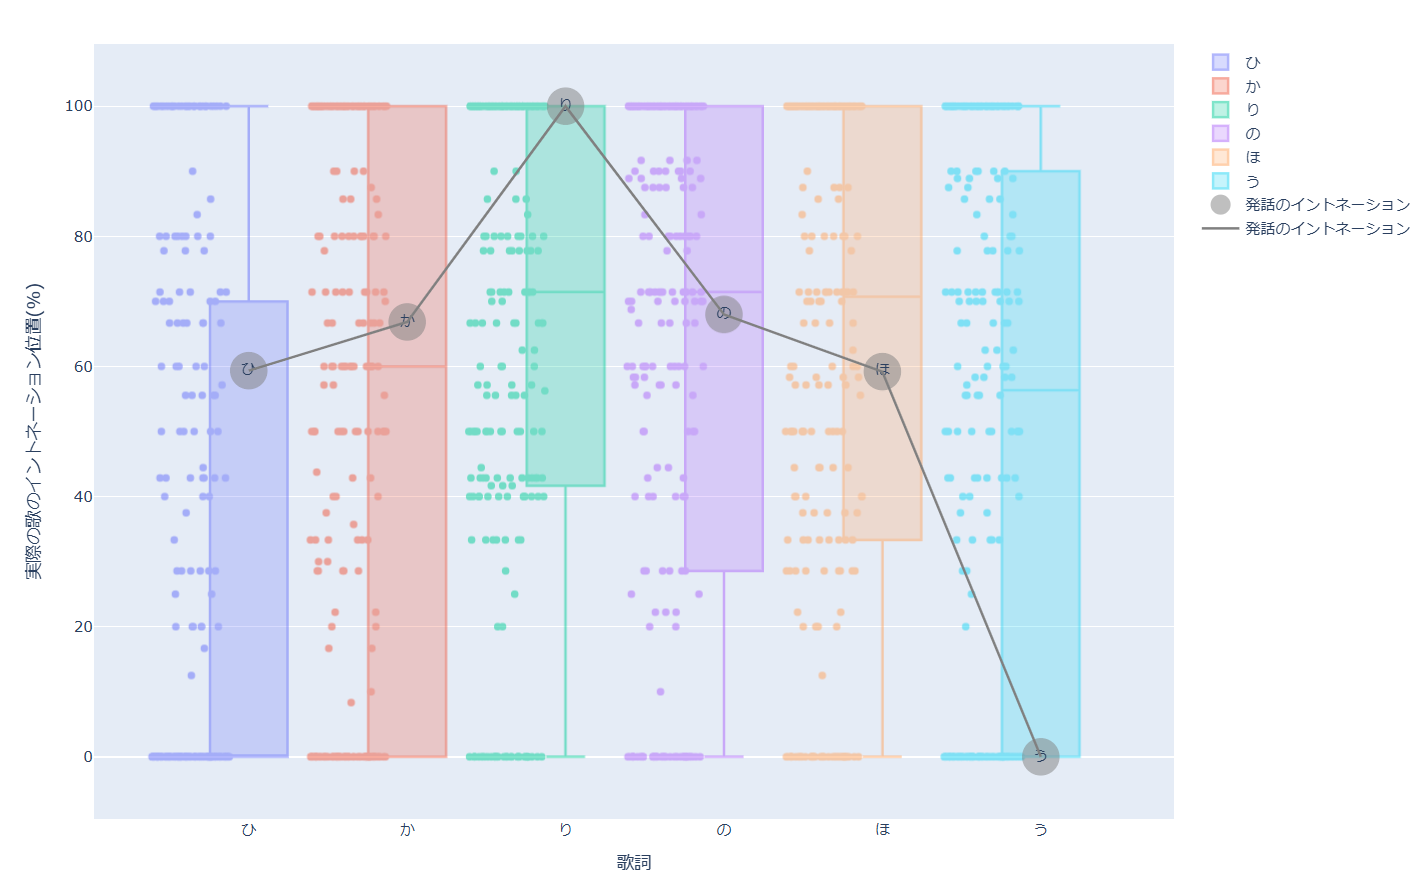
\includegraphics[width=\columnwidth]{fig/hikari/hakohige_into.png}
%  \caption{発話イントネーションと歌のずれ（ひ）}
%  \label{h_ha_into}
%\end{figure}

%4.3.3
\subsubsection{タイミングとイントネーションの比較}\label{sec:4.3.3}
\ref{sec:4.3.1}と\ref{sec:4.3.2}で出した各単音の割合を元に，それぞれのフレーズの全体でどれだけタイミングとイントネーションがずれているのかを散布図でプロットした．x軸がタイミングとの乖離度，y軸がイントネーションとの乖離度を表している．\par

\textbf{“あなたにあいたくて”での結果}\par
\figref{a_bunpu}より，イントネーションの乖離度は10\%付近から60\%付近までばらつきがあるが，タイミングの乖離度はおおむね10\%ほどでおさまっていることがわかる．\par
%\begin{figure}[tb]
%  \centering
%  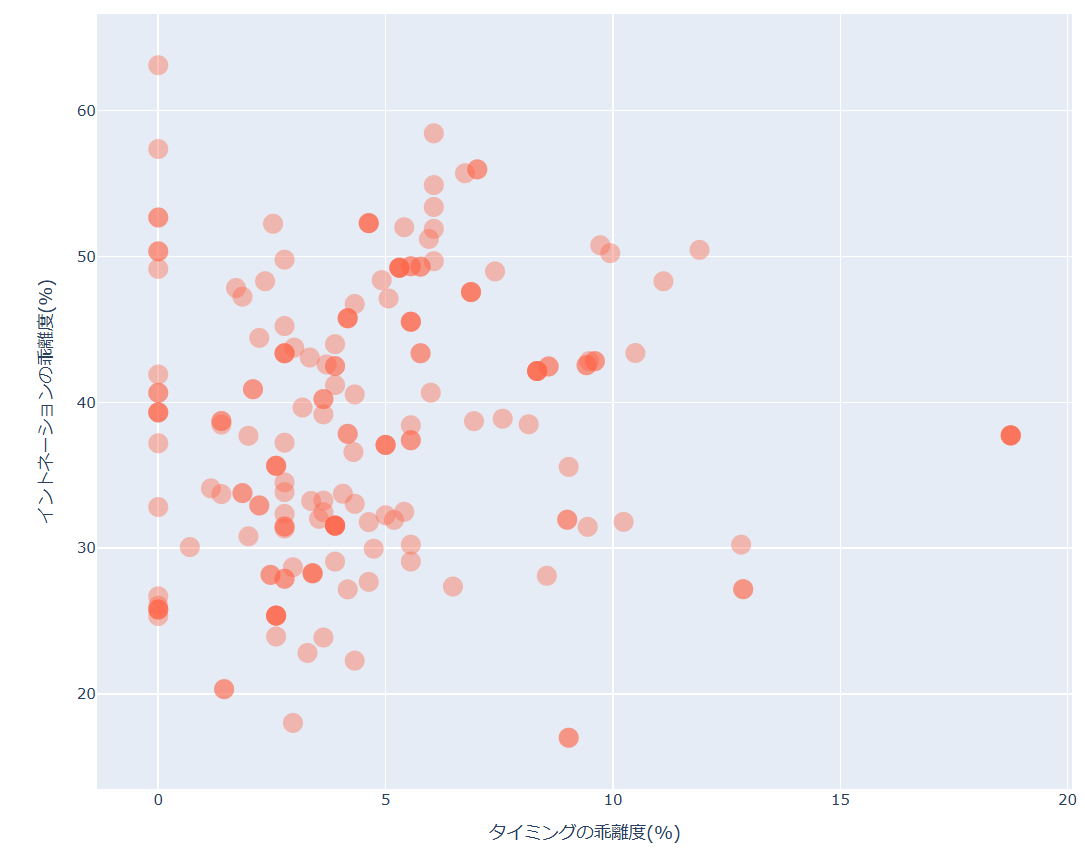
\includegraphics[width=\columnwidth]{fig/anata/bunpu.png}
%  \caption{タイミングとイントネーションのずれ（あ）}
%  \label{a_bunpu}
%\end{figure}

\textbf{“ひかりのほう”での結果}\par
\figref{h_bunpu}より，イントネーションの乖離度は0\%から75\%付近までばらつきがあり，タイミングの乖離度は0\%付近から15.5\%ほどであるとわかる．
また，タイミングの乖離度が0\%の位置，つまり発話タイミングと同じタイミングで歌われている楽曲が固まっていることが，\figref{h_bunpu}からわかる．
そこで，0\%のタイミングのフレーズのみで，音高-拍及び音高-秒数のグラフを出した．それが\figref{0_soroe}である．\par
\figref{0_haku}より，“ひかりのほう”の発話タイミングと一致しているフレーズは，おおよそ3拍以内で歌われることがわかった．また，\figref{0_byou}より，一致いているフレーズは2秒までで歌い切られることが多く，最長でも約6秒で歌い切られていることがわかった．
%\red{これいる？高さは45から75，つまりA2からD\(\sharp \)5の間で歌われていることがわかった．}
\begin{figure*}[t]
  \centering
  \begin{minipage}{0.49\hsize}
    \centering
    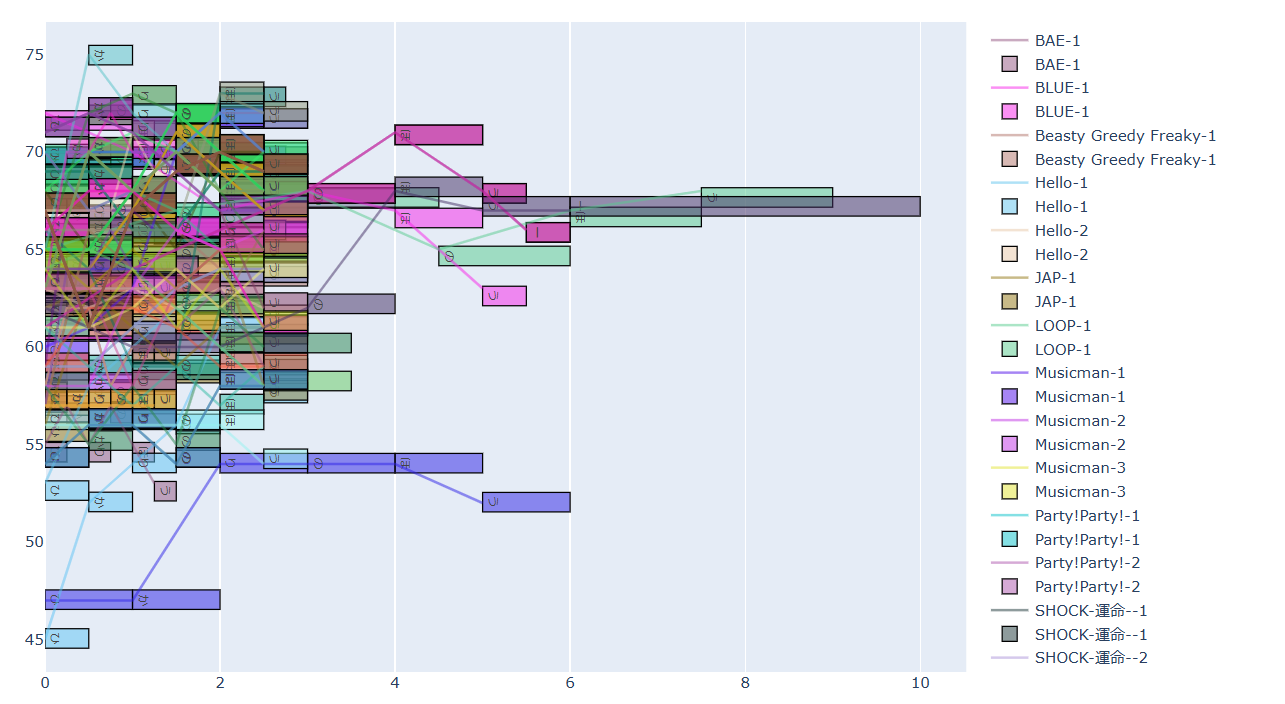
\includegraphics[width=.9\columnwidth]{fig/hikari/0_soroe.png}
    \subcaption{タイミングが完全一致の音高-拍グラフ}
    \label{0_haku}
  \end{minipage}
  \begin{minipage}{0.49\hsize}
    \centering
    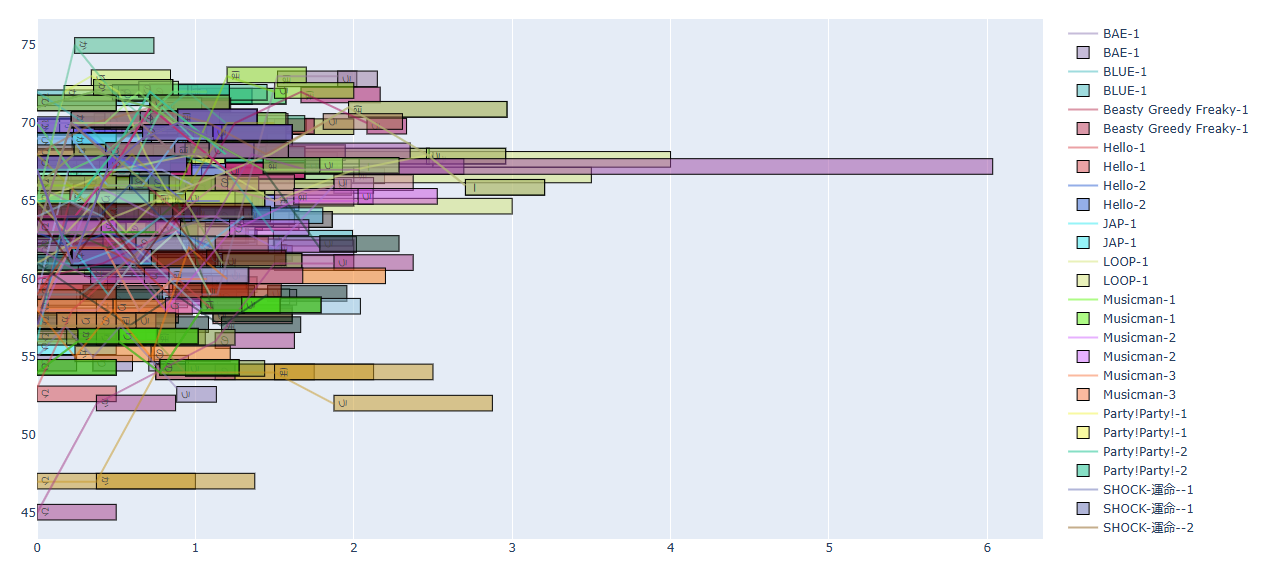
\includegraphics[width=\columnwidth]{fig/hikari/0_byou.png}
    \subcaption{タイミングが完全一致の音高-秒数グラフ}
    \label{0_byou}
  \end{minipage}
  \caption{タイミングが完全一致のグラフ}
  \label{0_score}
\end{figure*}


%4.3
\subsection{歌手の性別ごとの傾向}
次に，歌手の性別ごとの発話表現との一致度について記していく．


%4.3.1
\subsubsection{男女別・単体or混合の全体に占める割合}
\begin{figure*}[t]
  \centering
  \begin{minipage}{0.49\hsize}
    \centering
    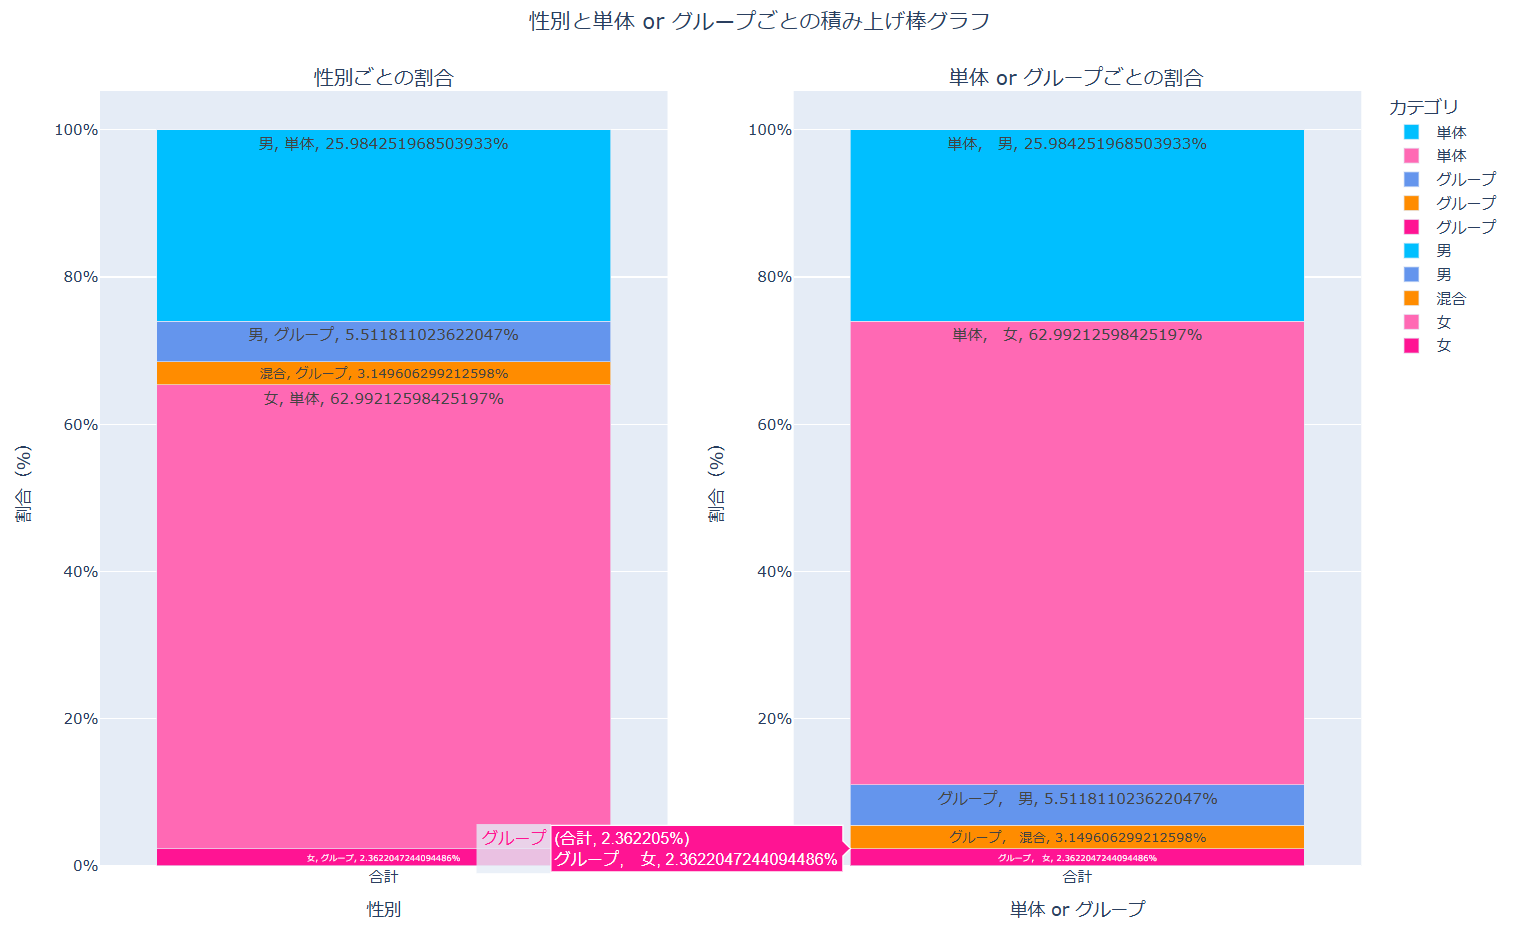
\includegraphics[width=.9\columnwidth]{fig/anata/seibetu_wariai.png}
    \subcaption{“あなたにあいたくて”}
    \label{a_seibetu_wari}
  \end{minipage}
  \begin{minipage}{0.49\hsize}
    \centering
    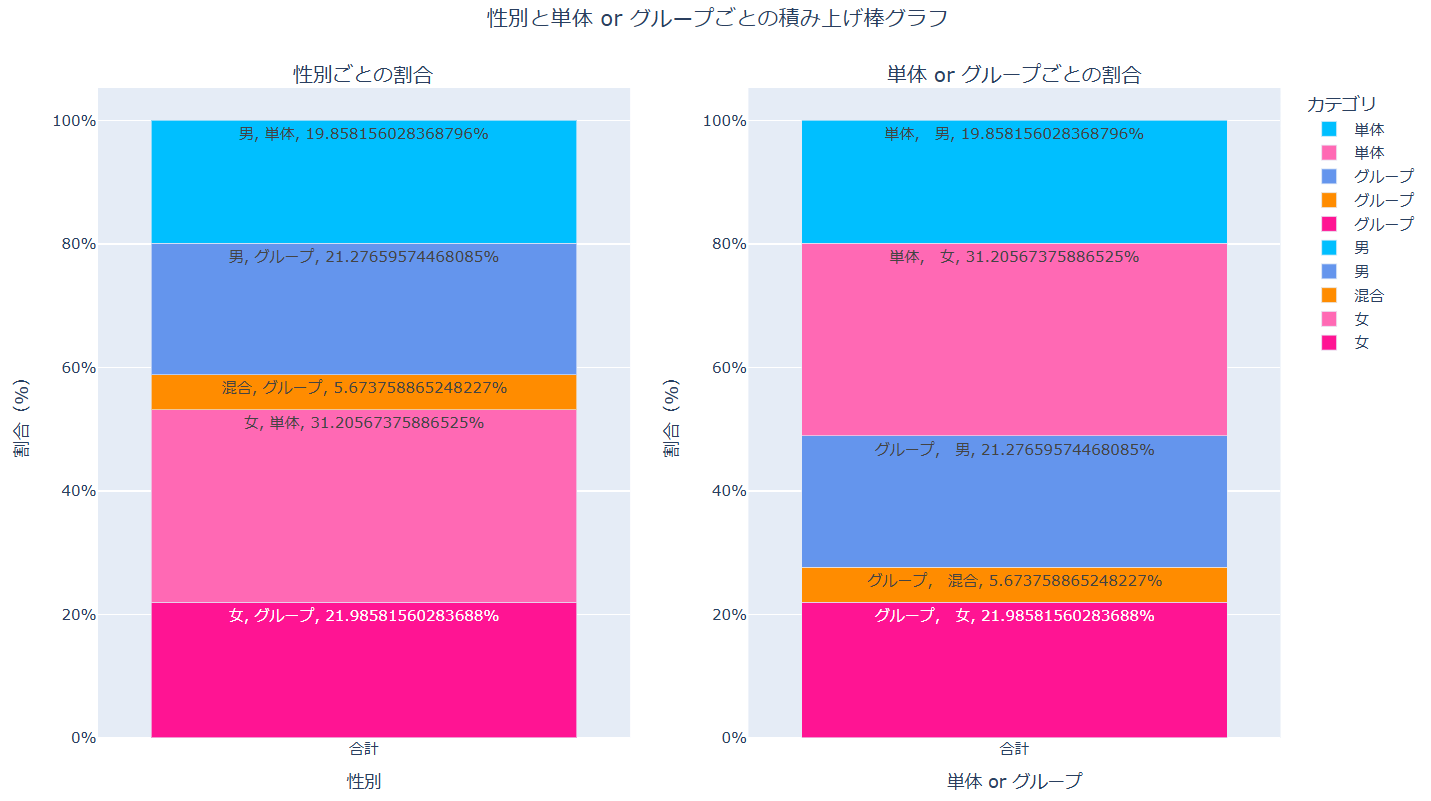
\includegraphics[width=\columnwidth]{fig/hikari/seibetu_wariai.png}
    \subcaption{“ひかりのほう”}
    \label{h_seibetu_wari}
  \end{minipage}
  \caption{性別ごとの全体の割合}
  \label{seibetu_wari}
\end{figure*}



\begin{figure*}[t]
  \centering
  \begin{minipage}{\hsize}
    \centering
    \begin{minipage}{0.3\hsize}
      \centering
      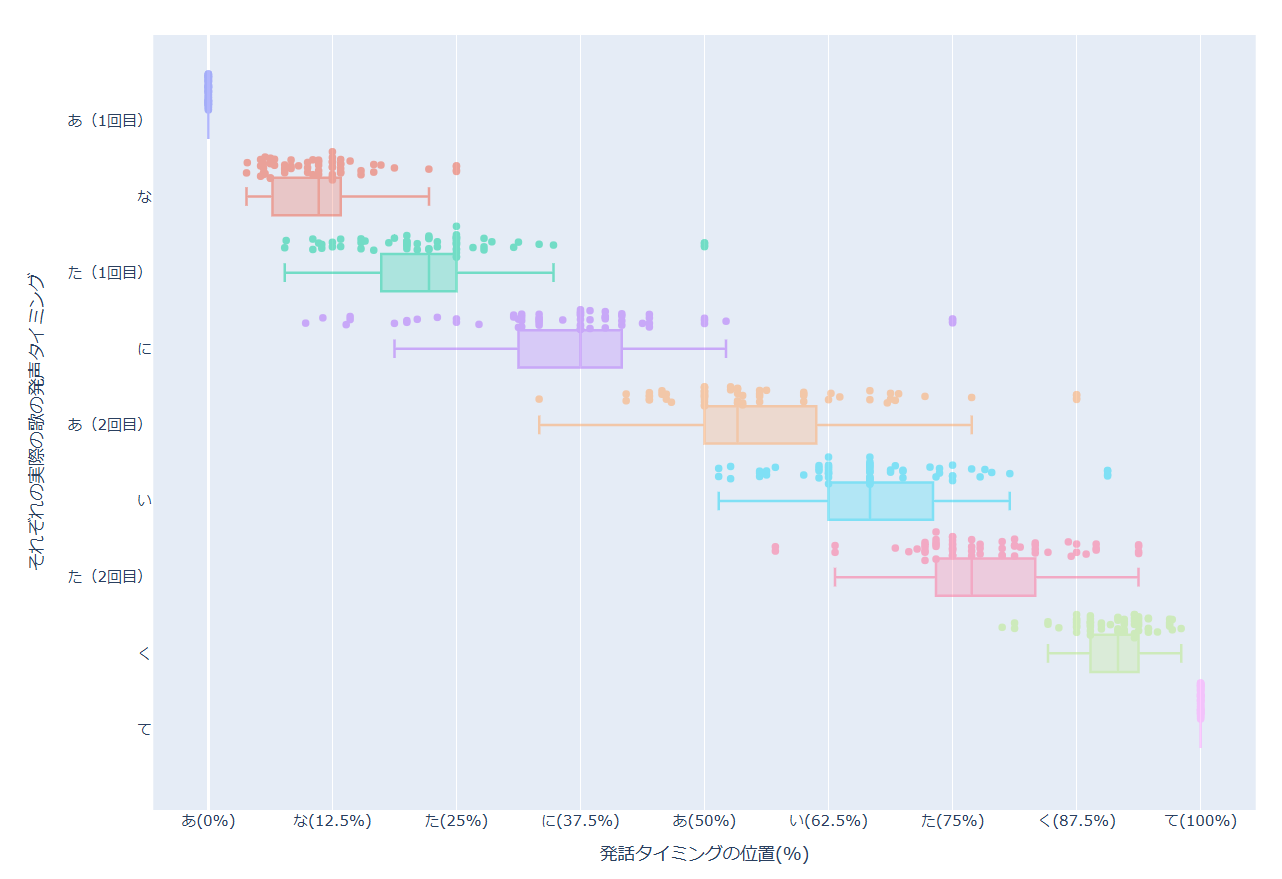
\includegraphics[width=\columnwidth]{fig/anata/otoko/tai.png}
      \subcaption{タイミングの違い}
      \label{a_otoko_tai}
    \end{minipage}
    \begin{minipage}{0.3\hsize}
      \centering
      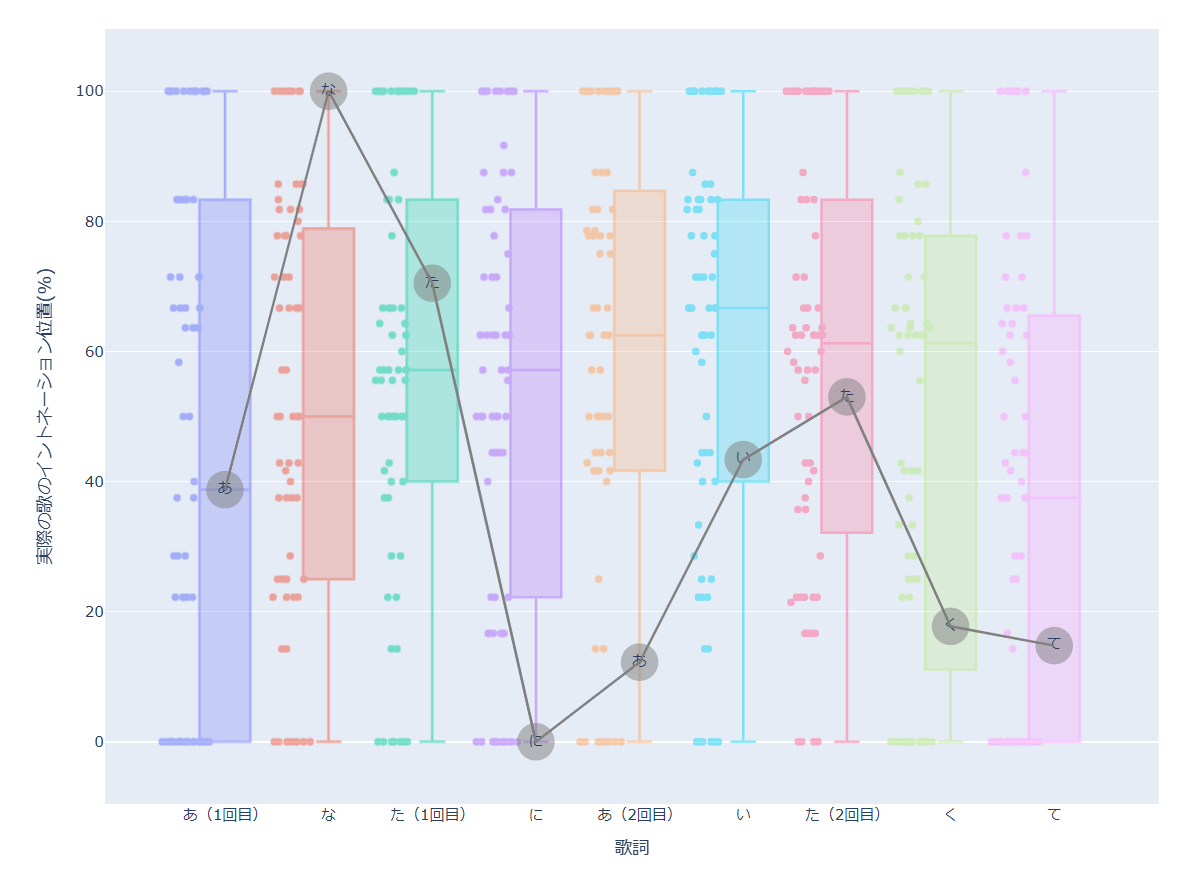
\includegraphics[width=.95\columnwidth]{fig/anata/otoko/int.png}
      \subcaption{イントネーションの違い}
      \label{a_otoko_int}
    \end{minipage}
    \begin{minipage}{0.3\hsize}
      \centering
      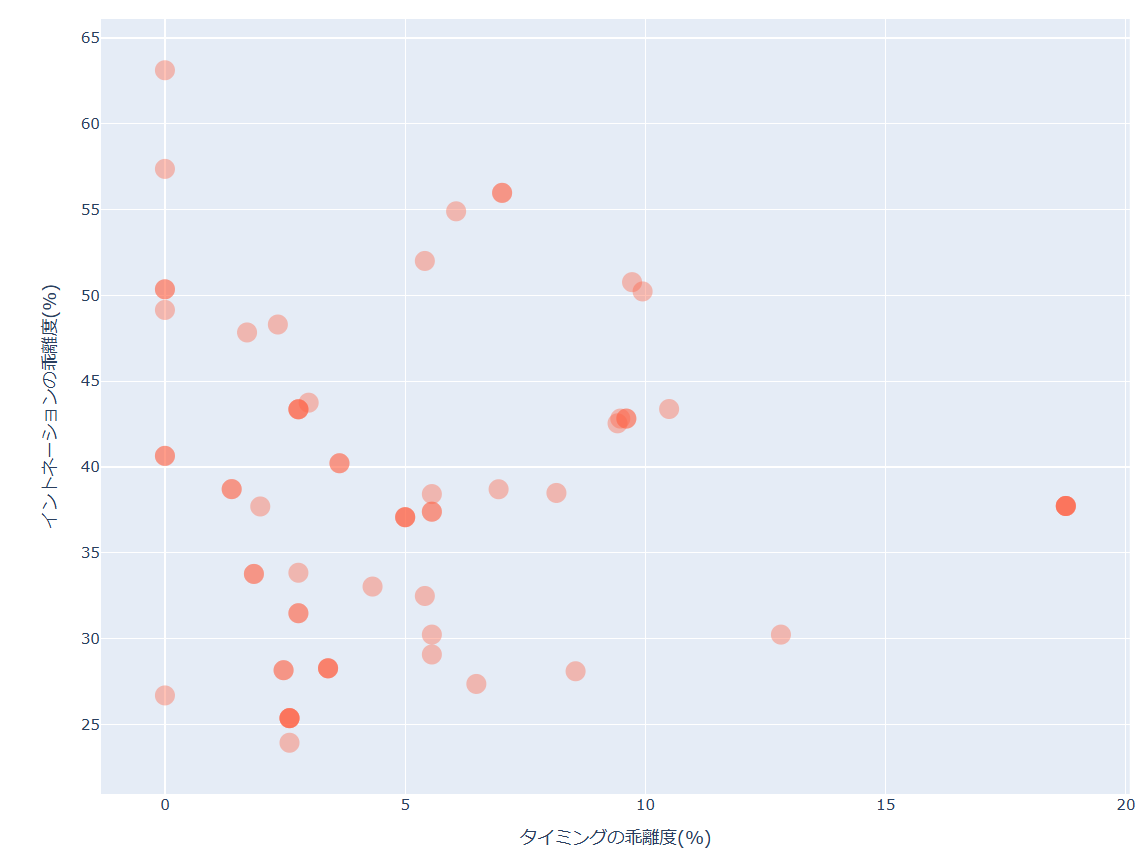
\includegraphics[width=\columnwidth]{fig/anata/otoko/tai_int.png}
      \subcaption{タイミングとイントネーションの乖離}
      \label{a_otoko_tai_int}
    \end{minipage}
    \caption{「あなたにあいたくて」の男性での発話表現との比較}
    \label{a_otoko_hakohige}
  \end{minipage}
  \begin{minipage}{\hsize}
    \centering
    \begin{minipage}{0.3\hsize}
      \centering
      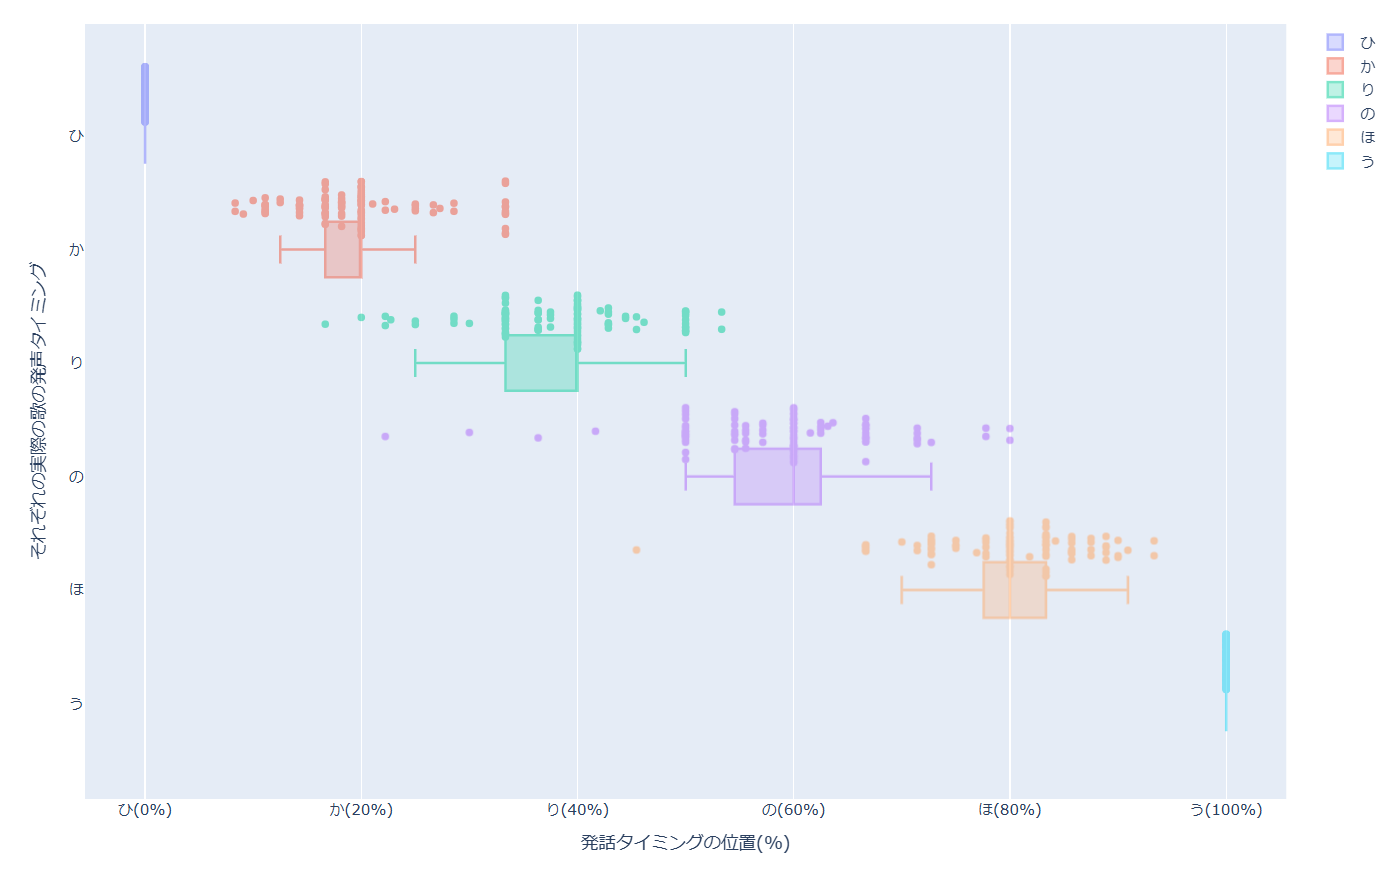
\includegraphics[width=\columnwidth]{fig/hikari/otoko/tai.png}
      \subcaption{タイミングの違い}
      \label{h_otoko_tai}
    \end{minipage}
    \begin{minipage}{0.3\hsize}
      \centering
      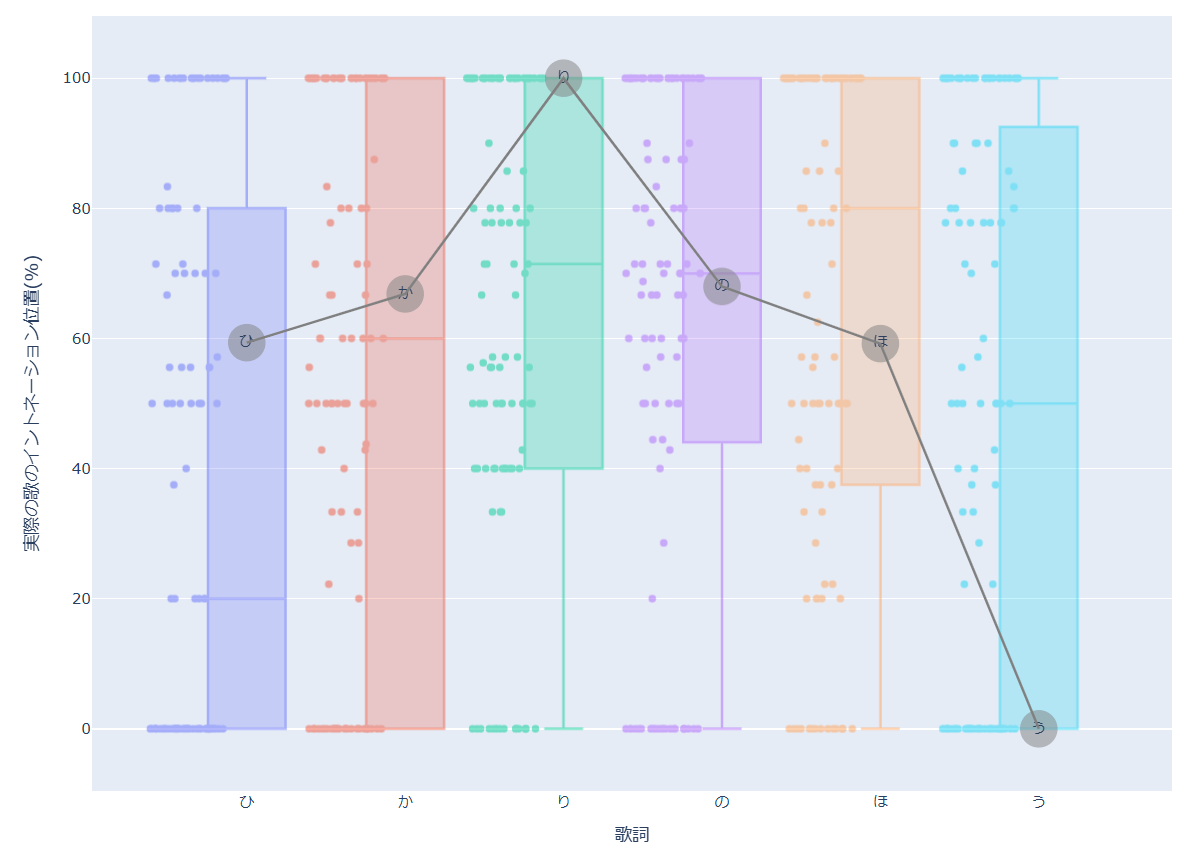
\includegraphics[width=\columnwidth]{fig/hikari/otoko/int.png}
      \subcaption{イントネーションの違い}
      \label{h_otoko_int}
    \end{minipage}
    \begin{minipage}{0.3\hsize}
      \centering
      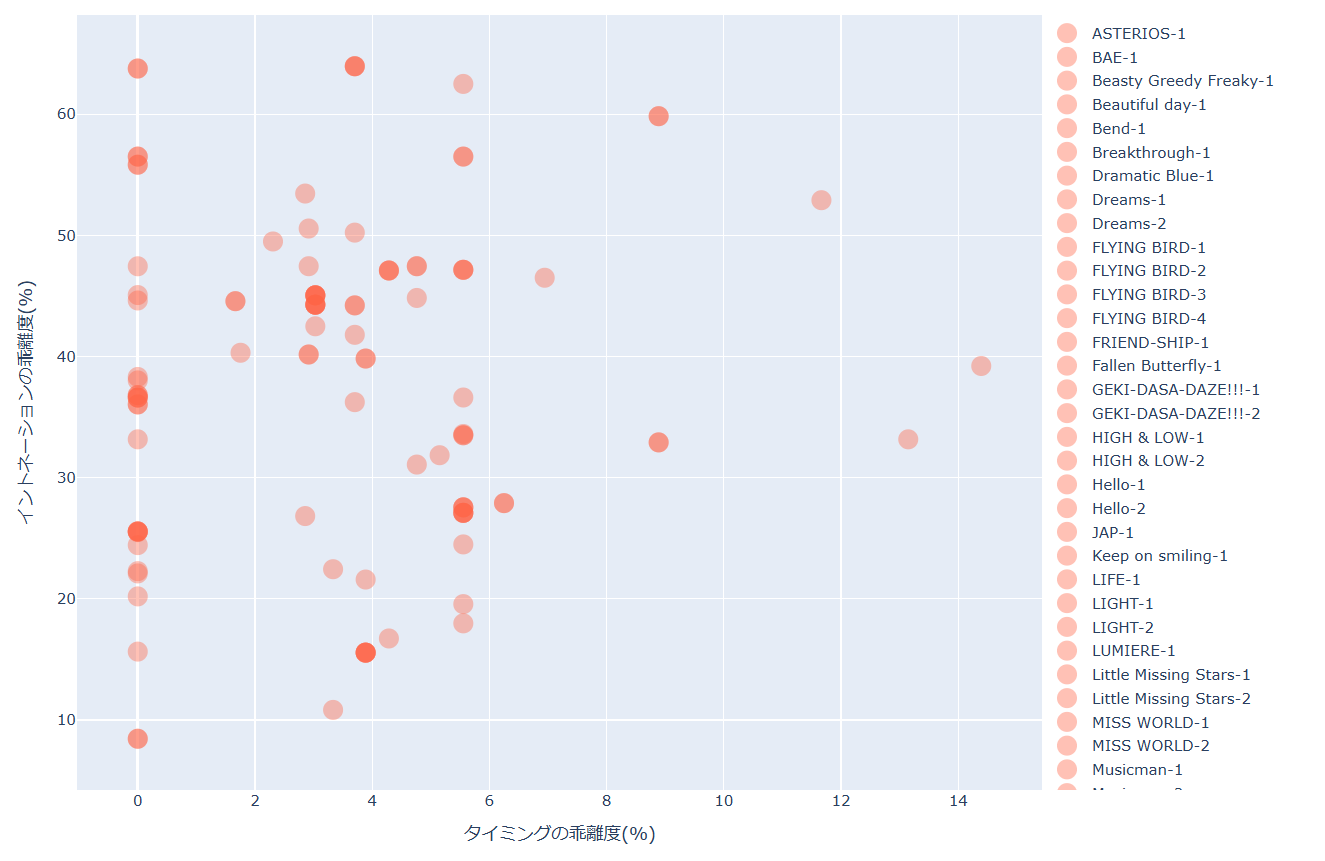
\includegraphics[width=\columnwidth]{fig/hikari/otoko/tai_int.png}
      \subcaption{タイミングとイントネーションの乖離}
      \label{h_otoko_tai_int}
    \end{minipage}
    \caption{「ひかりのほう」の男性での発話表現との比較}
    \label{h_otoko_hakohige}
  \end{minipage}
  \begin{minipage}{\hsize}
    \centering
    \begin{minipage}{0.3\hsize}
      \centering
      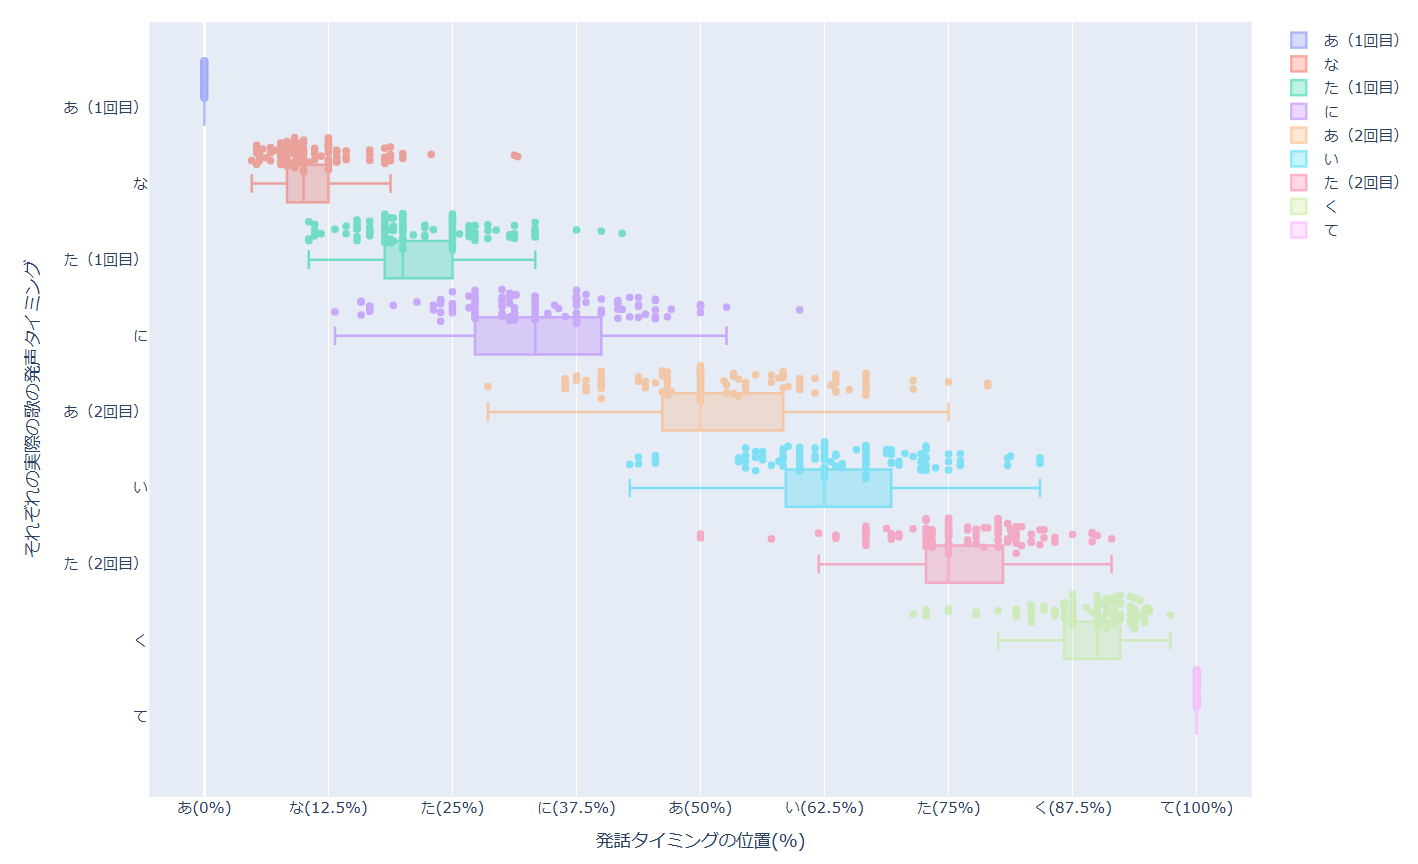
\includegraphics[width=\columnwidth]{fig/anata/onna/tai.png}
      \subcaption{タイミングの違い}
      \label{a_onna_tai}
    \end{minipage}
    \begin{minipage}{0.3\hsize}
      \centering
      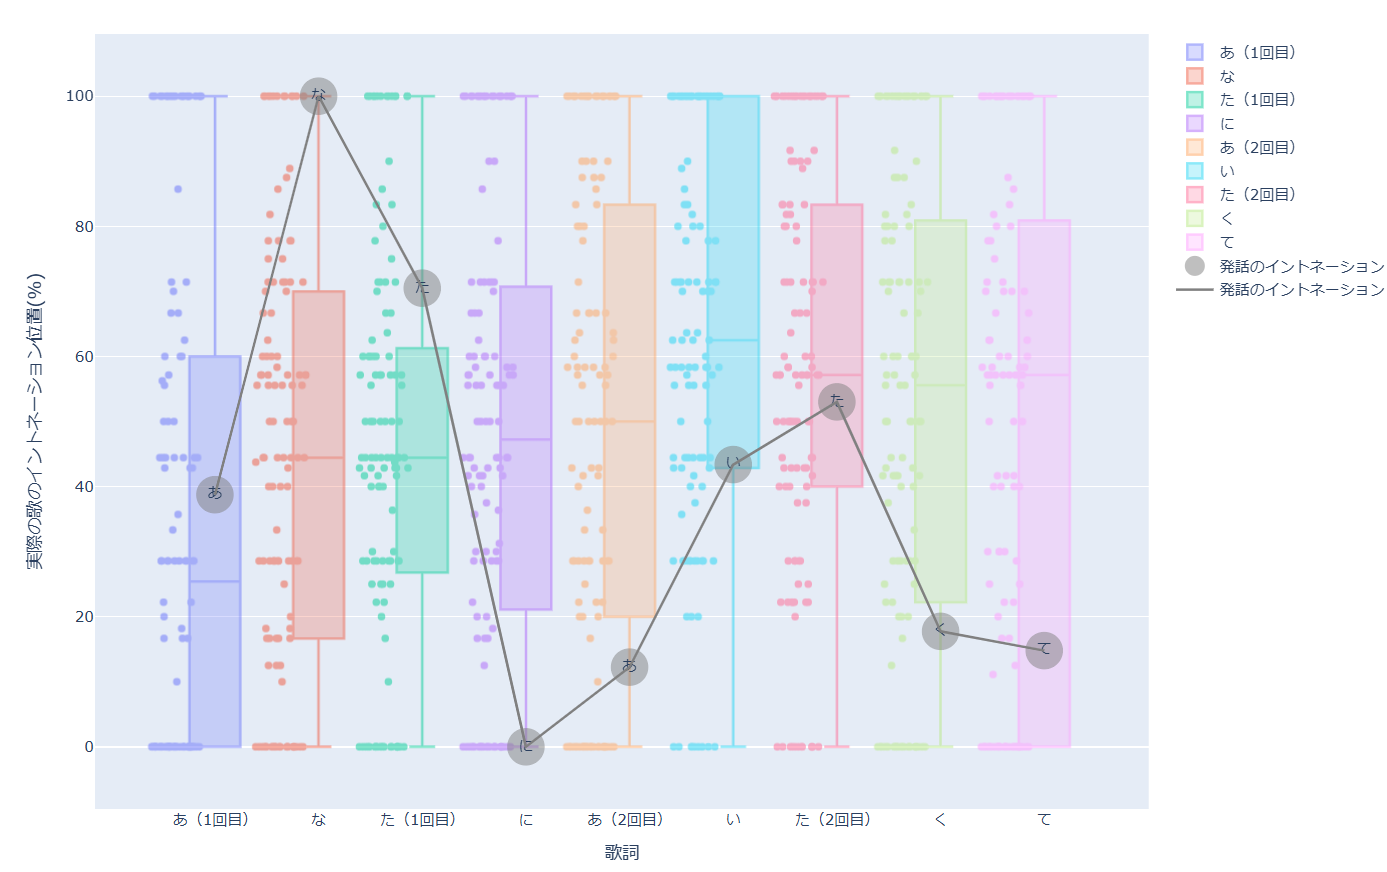
\includegraphics[width=\columnwidth]{fig/anata/onna/int.png}
      \subcaption{イントネーションの違い}
      \label{a_onna_int}
    \end{minipage}
    \begin{minipage}{0.3\hsize}
      \centering
      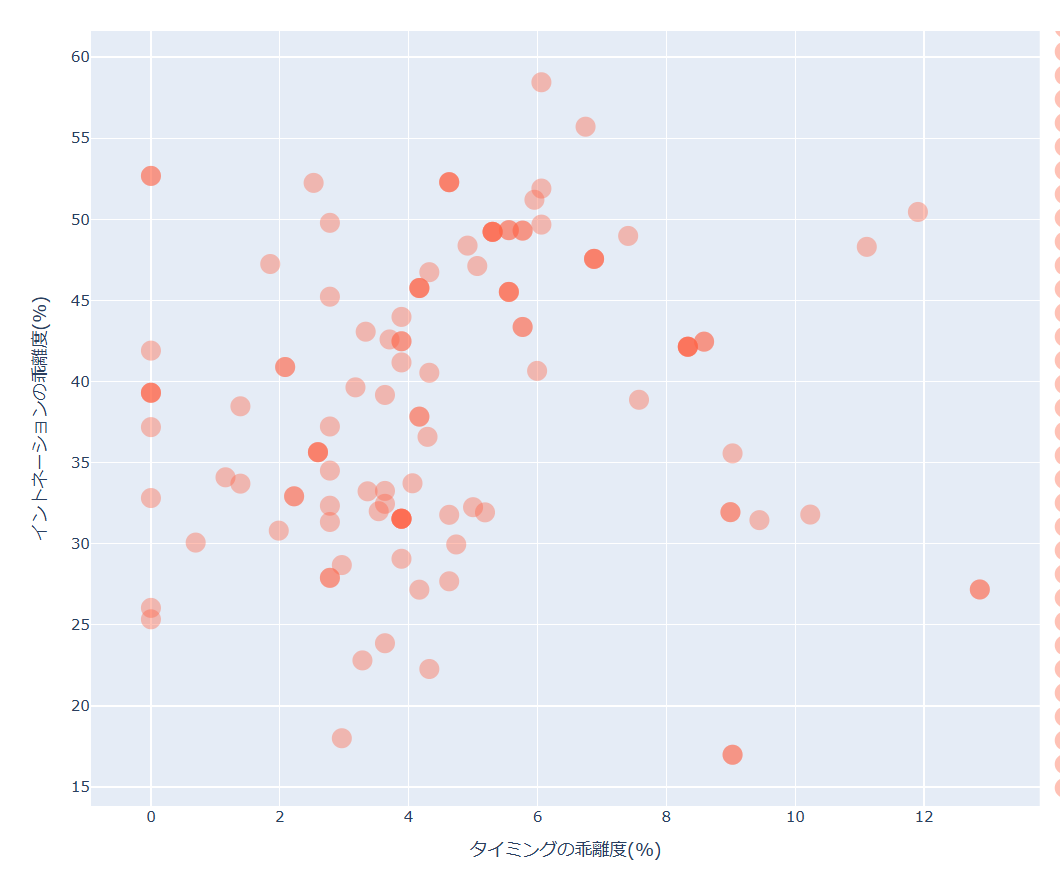
\includegraphics[width=\columnwidth]{fig/anata/onna/tai_int.png}
      \subcaption{タイミングとイントネーションの乖離}
      \label{a_onna_tai_int}
    \end{minipage}
    \caption{「あなたにあいたくて」の女性での発話表現との比較}
    \label{a_onna_hakohige}
  \end{minipage}
  \begin{minipage}{\hsize}
    \centering
    \begin{minipage}{0.3\hsize}
      \centering
      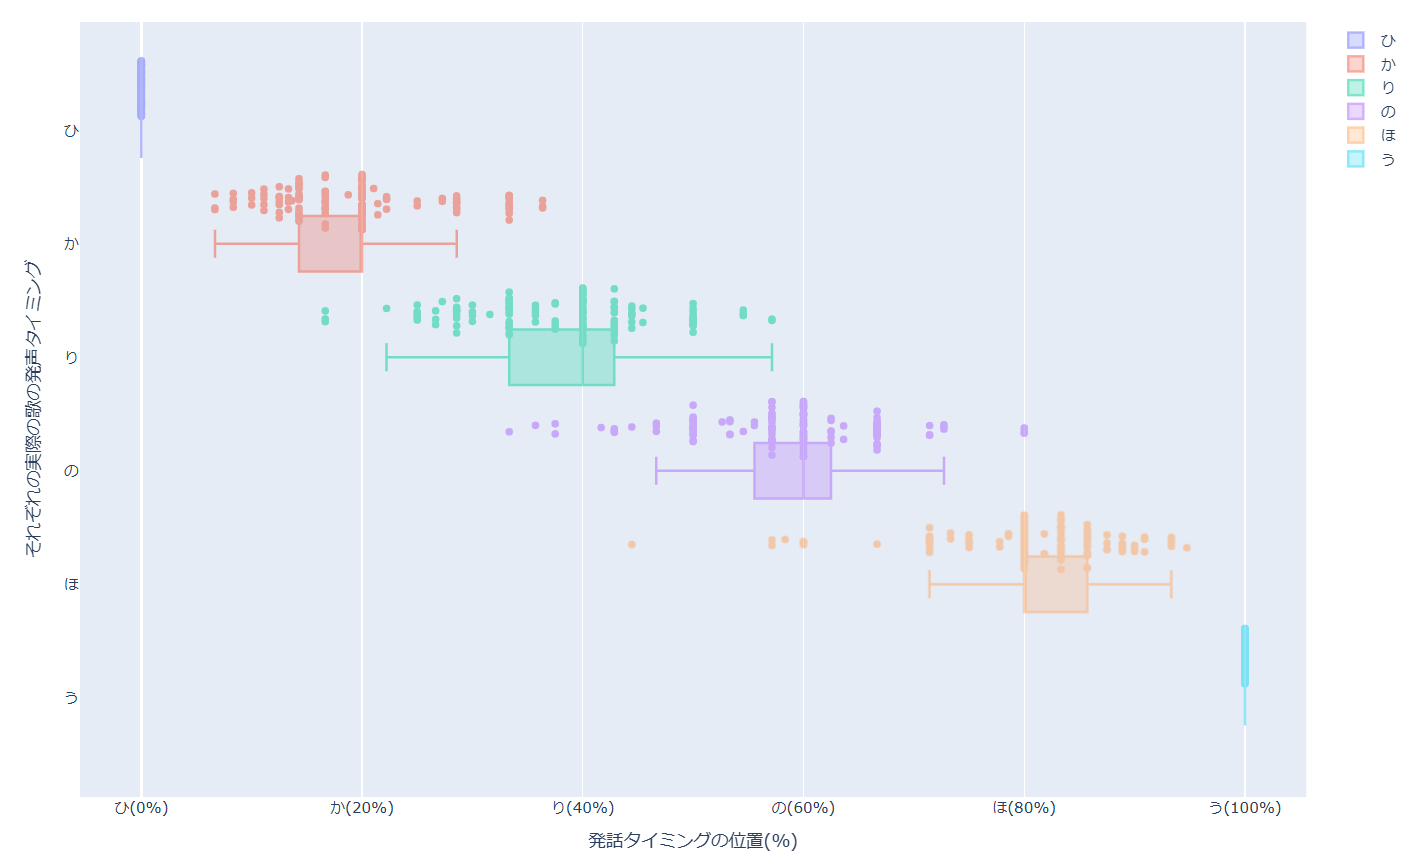
\includegraphics[width=\columnwidth]{fig/hikari/onna/tai.png}
      \subcaption{タイミングの違い}
      \label{h_onna_tai}
    \end{minipage}
    \begin{minipage}{0.3\hsize}
      \centering
      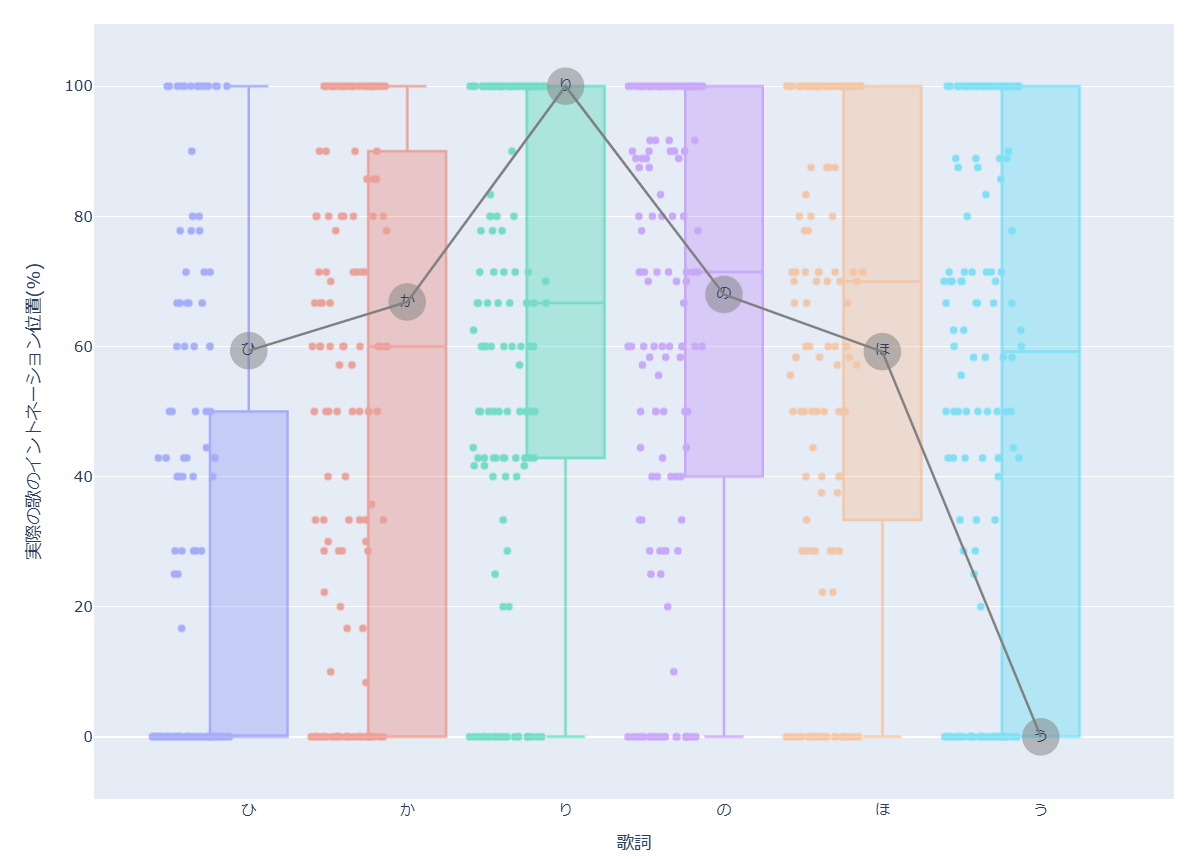
\includegraphics[width=\columnwidth]{fig/hikari/onna/int.png}
      \subcaption{イントネーションの違い}
      \label{h_onna_int}
    \end{minipage}
    \begin{minipage}{0.3\hsize}
      \centering
      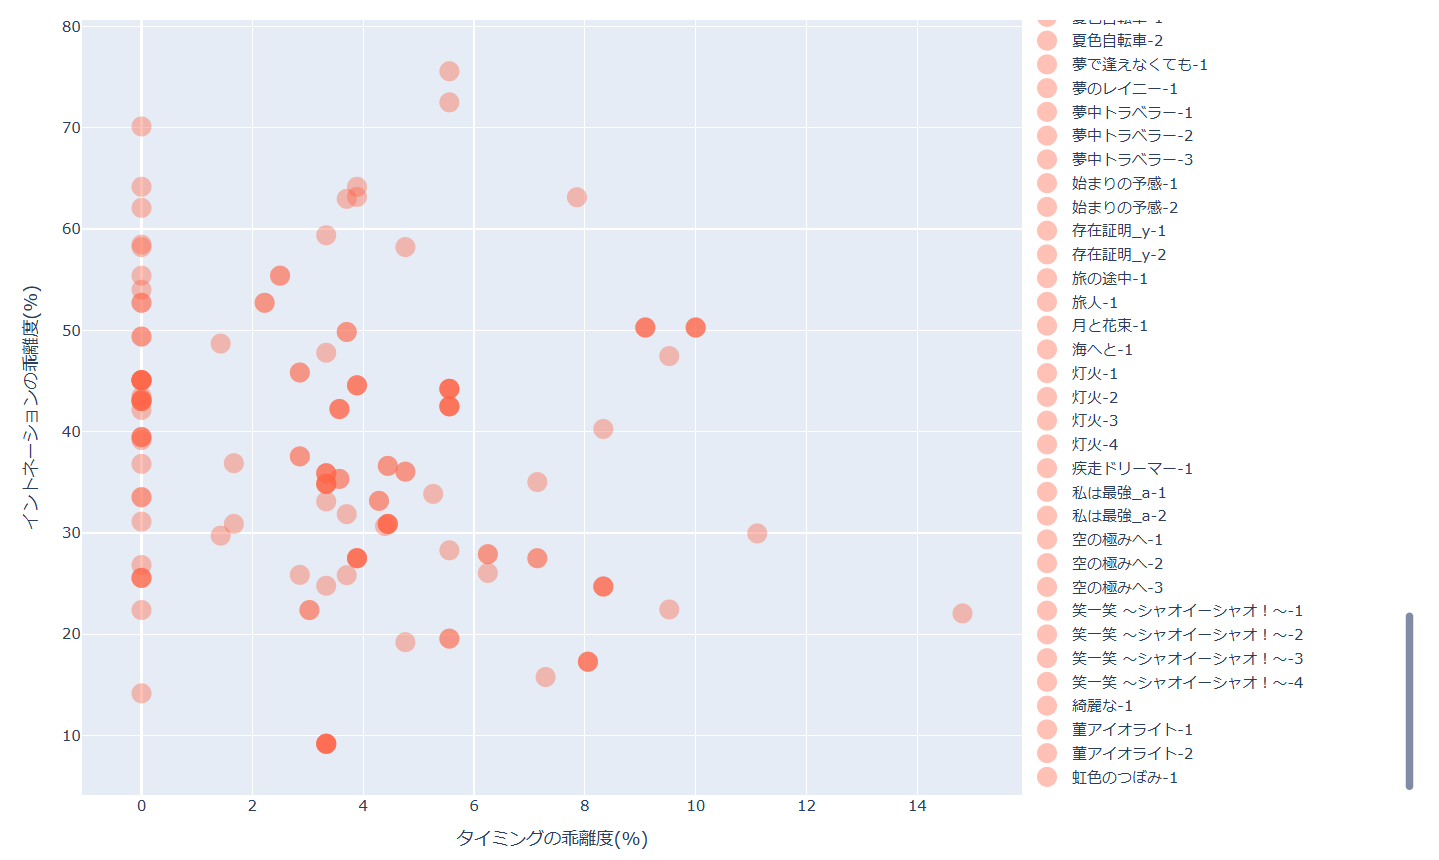
\includegraphics[width=\columnwidth]{fig/hikari/onna/tai_int.png}
      \subcaption{タイミングとイントネーションの乖離}
      \label{h_onna_tai_int}
    \end{minipage}
    \caption{「ひかりのほう」の女性での発話表現との比較}
    \label{h_onna_hakohige}
  \end{minipage}
\end{figure*}



\textbf{“あなたにあいたくて”での結果}\par
「あなたにあいたくて」フレーズを歌っている歌手の男女の割合，人数の割合が\figref{a_seibetu_wari}である，\par
性別では，女性が約65\%を，男性が約31\%を，男女混合が約3\%の楽曲を歌っていることがわかった．\par
人数では，単体（1人）が約90\%，グループ（複数人）が10\%という結果になった．\par


\textbf{“ひかりのほう”での結果}\par
「ひかりのほう」フレーズを歌っている歌手の男女の割合，人数の割合が\figref{h_seibetu_wari}である，\par
性別別に見ると，女性が約52\%を，男性が約44\%を，男女混合が約5\%の楽曲を歌っていることがわかった．\par
人数では，単体（1人）が約54\%，グループ（複数人）が45\%という結果になった．

%4.3.2
\subsubsection{男}
各フレーズを男性が歌っているものに絞り，発話表現との比較を行ったのが\figref{a_otoko_hakohige}，\figref{h_otoko_hakohige}である．
%各フレーズを男性が歌っているものでそれぞれプロットしたものが\figref{a_otoko},\figref{h_otoko}である．\par

\textbf{“あなたにあいたくて”での結果}\par
%男性が歌っているものをプロットしたのが\figref{a_otoko}である．\par
%音長はおおよそ25拍以内で歌われている．また，音の高さはMIDIナンバーで45～73，つまりA2～C\(\sharp \)5の間で歌われており，男性の平均音域であるD3～A4\cite{dansei_oniki}より広い音域を歌っている．
\figref{a_otoko_tai}より，「に」において，中央値が一致していることがわかる．また，「た（1回目）」において，第三四分位数が発話タイミングと一致していることから，75\%は発話タイミングと同じか早く発音されていることがわかる．また，「あ（2回目）」「い」において，第一四分位数が発話タイミングと一致していることから，75\%は発話タイミングと同じか早く発音されていることがわかる．\par
また，\figref{a_otoko_int}において，「あ（1回目）」「て」において，最小値および第一四分位数が0の位置にあることから，各単音の少なくとも4分の1が0\%の位置で歌われていることがわかる．\par
さらに，\figref{a_otoko_tai_int}において，イントネーションの乖離度は0\%から63\%付近までばらつきがあり，タイミングの乖離度は0\%付近から18\%ほどであるとわかる．


\textbf{“ひかりのほう”での結果}\par
%男性が歌っているものをプロットしたのが\figref{h_otoko}である．\par
%音長は11拍以内で歌われている．また，音の高さはMIDIナンバーで45～73，つまりA2～C\(\sharp \)5の間で歌われており，男性の平均音域であるD3～A4より広い音域を歌っている．
\figref{h_otoko_tai}より，\ref{sec:4.3.1}節と同じく「ひかりのほう」は全て単音において，中央値とタイミングが一致していることがわかる．また，「か」「り」において，第三四分位数が中央値および発話タイミングと一致していることから，75\%は発話タイミングと同じか早く発音されており，その中でも50\%から75\%に分布している，つまり25\%は発話タイミングと一致して発音されていることがわかる．また，「の」と「ほ」において，2つ前の単音の発話タイミングの位置付近まで外れ値があることがわかる．\par
また，\figref{h_otoko_int}において，「か」「り」「の」「ほ」において，最大値および第三四分位数が100\%にあることから，各単音の最低でも4分の1がフレーズ内の最も高い音で歌われていることがわかる．\par
また，「ひ」「か」「う」において，最小値および第一四分位数が0の位置にあることから，各単音の少なくとも4分の1が0\%の位置で歌われていることがわかる．\par
さらに，\figref{h_otoko_tai_int}において，イントネーションの乖離度は0\%から75\%付近までばらつきがあり，タイミングの乖離度は0\%付近から15.5\%ほどであるとわかる．また，\ref{sec:4.3.3}と同じく，タイミングの乖離度が0\%の位置，つまり発話タイミングと同じタイミングで歌われている楽曲が固まっていることがわかる．


\begin{figure*}[t]
  \centering
  \begin{minipage}{0.3\hsize}
    \centering
    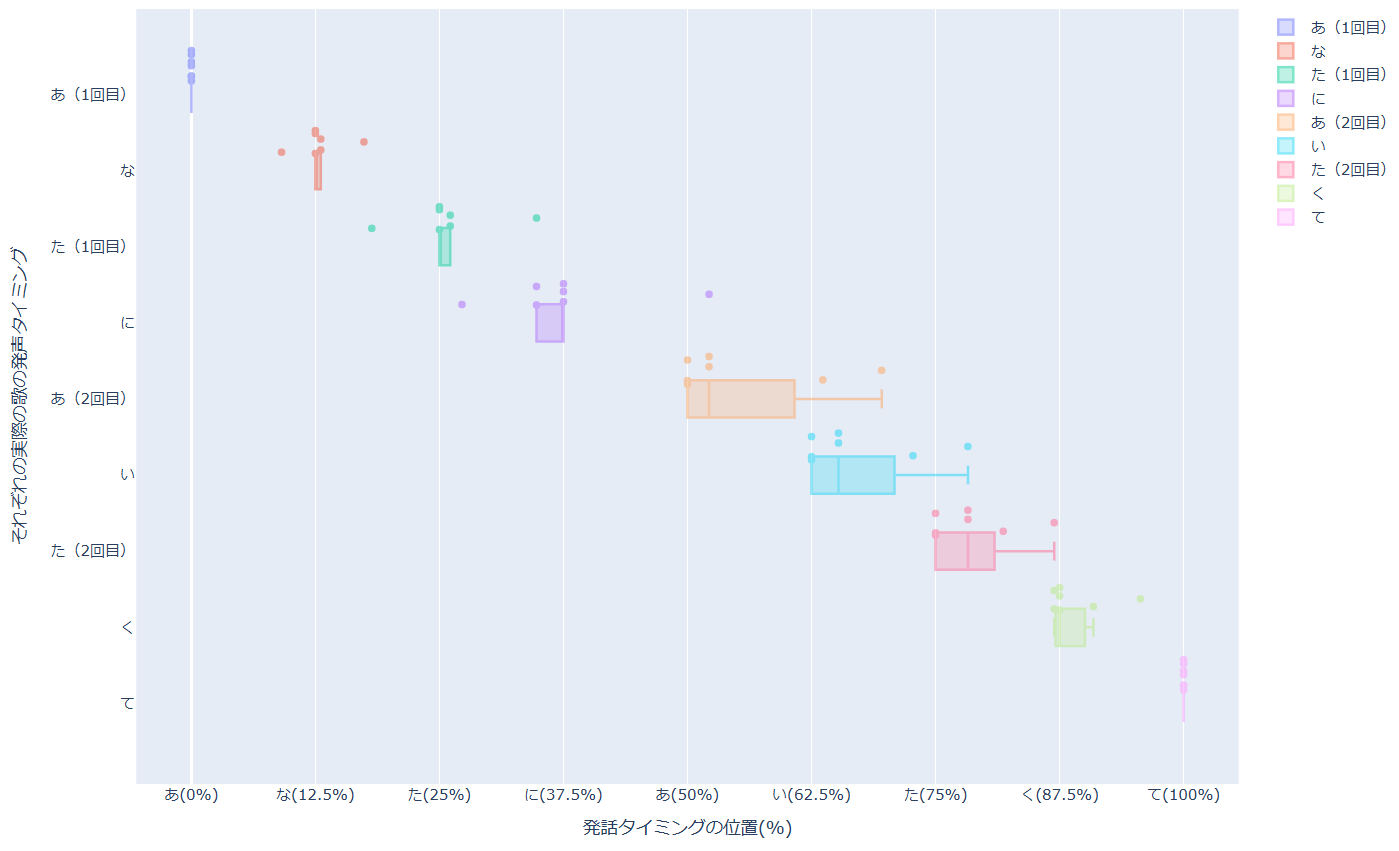
\includegraphics[width=\columnwidth]{fig/anata/kongo/tai.png}
    \subcaption{混合でのタイミングの違い}
    \label{a_kongo_tai}
  \end{minipage}
  \begin{minipage}{0.3\hsize}
    \centering
    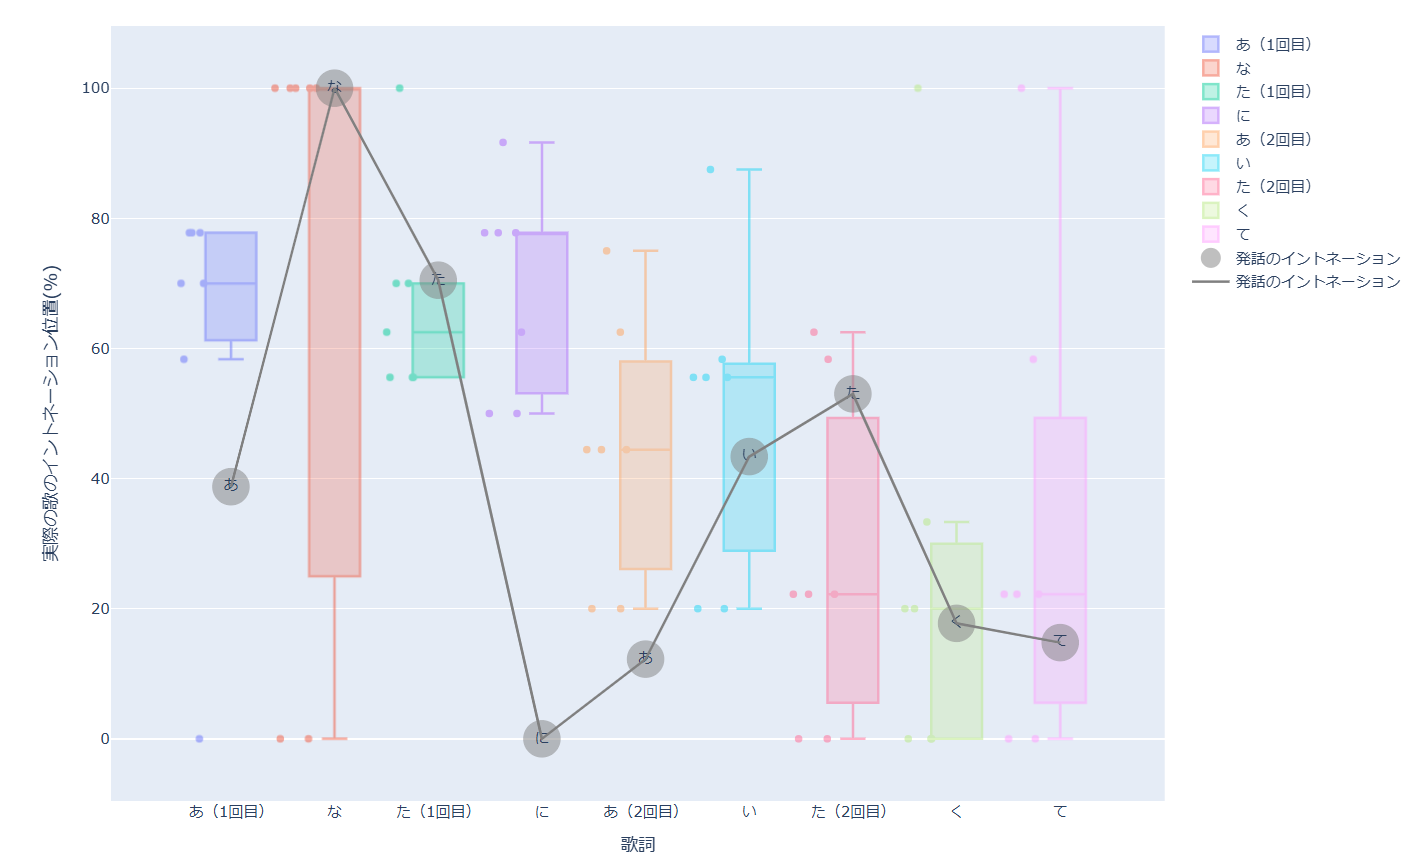
\includegraphics[width=\columnwidth]{fig/anata/kongo/int.png}
    \subcaption{混合でのイントネーションの違い}
    \label{a_kongo_int}
  \end{minipage}
  \begin{minipage}{0.3\hsize}
    \centering
    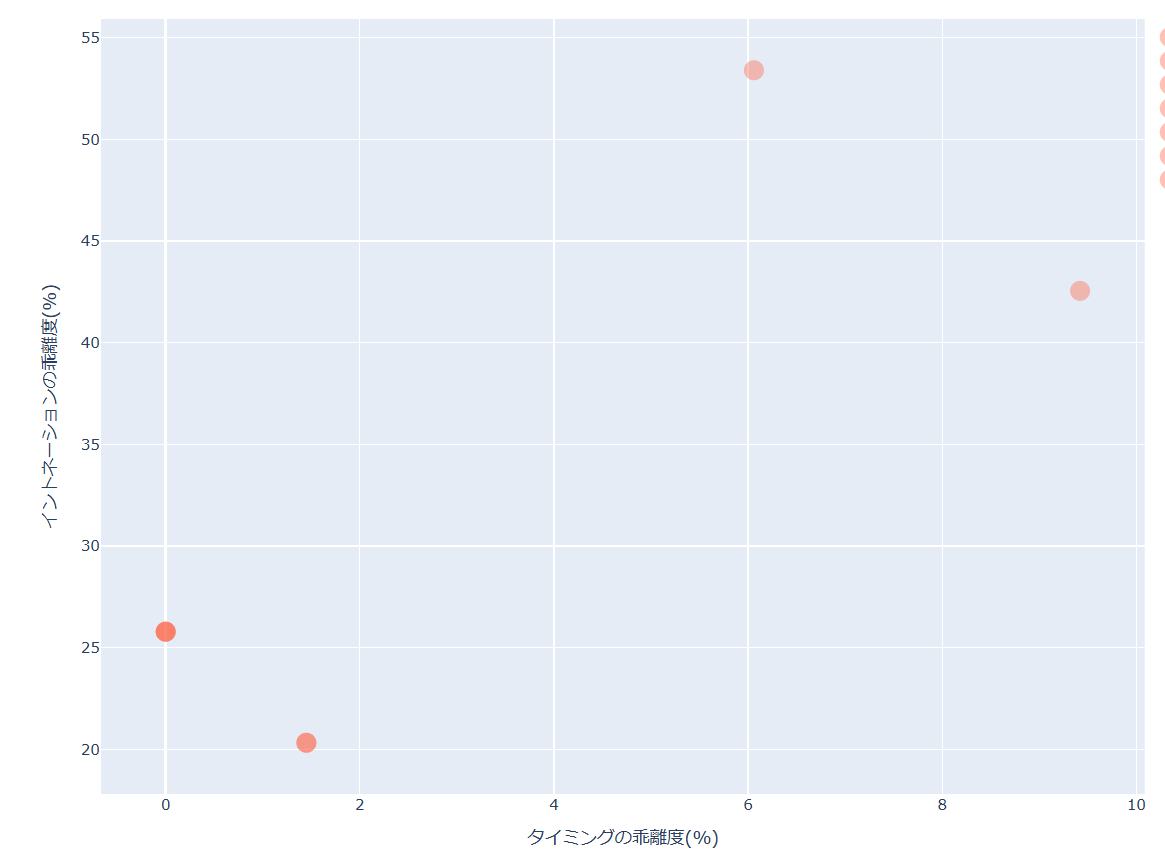
\includegraphics[width=\columnwidth]{fig/anata/kongo/tai_int.png}
    \subcaption{混合でのタイミングとイントネーションの乖離}
    \label{a_kongo_tai_int}
  \end{minipage}
  \caption{「あなたにあいたくて」の混合での発話表現との比較}
  \label{a_kongo_hakohige}
\end{figure*}





%4.3.3
\subsubsection{女}
各フレーズを女性が歌っているものでそれぞれプロットしたものが\figref{a_onna},\figref{h_onna}である．\par


\textbf{“あなたにあいたくて”での結果}\par
\figref{a_onna_tai}より，「あ（2回目）」「い」「た（2回目）」において，中央値が一致していることがわかる．また，「な」と「た（1回目）」において，第三四分位数が発話タイミングと一致していることから，75\%は発話タイミングと同じか早く発音されていることがわかる．\par
また，\figref{a_onna_int}において，「あ（1回目）」「て」において，最小値および第一四分位数が0\%の位置にあることから，各単音の少なくとも4分の1がフレーズ内の最も低い音で歌われていることがわかる．また，「い」において，最大値および第三四分位数が100\%の位置にあることから，少なくとも4分の1がフレーズ内の最も高い音で歌われていることがわかる．\par
さらに，\figref{a_onna_tai_int}において，イントネーションの乖離度は0\%から58\%付近までばらつきがあり，タイミングの乖離度は0\%付近から13\%ほどであるとわかる．
%女性が歌っているものをプロットしたのが\figref{a_onna}である．\par
%音長はおおよそ25拍以内で歌われている．また，音の高さはMIDIナンバーで54～76，つまりF\(\sharp \)3～E5の間で歌われており，女性の平均音域であるG3～D5\cite{zyosei_oniki}より広い音域を歌っている．


\textbf{“ひかりのほう”での結果}\par
%女性が歌っているものをプロットしたのが\figref{h_onna}である．\par
%音長はおおよそ12拍以内で歌われている．また，音の高さはMIDIナンバーで52～77，つまりE3～F5の間で歌われており，女性の平均音域であるG3～D5より広い音域を歌っている．
\figref{h_onna_tai}より，\ref{sec:4.3.1}節と同じく「ひかりのほう」は全て単音において，中央値とタイミングが一致していることがわかる．また，「か」において第三四分位数が中央値および発話タイミングと一致していることから，75\%は発話タイミングと同じか早く発音されており，その中でも50\%から75\%に分布している，つまり25\%は発話タイミングと一致して発音されていることがわかる．また，「ほ」において，第一四分位数が中央値および発話タイミングと一致していることから，75\%は発話タイミングと同じか遅く発音されており，その中でも25\%から50\%に分布している，つまり25\%は発話タイミングと一致して発音されていることがわかる．また，「ほ」において，2つ前の単音の発話タイミングの位置付近まで外れ値があることがわかる．\par
また，\figref{h_onna_int}において，「り」「の」「ほ」「う」において，第一四分位数が100\%にあることから，各単音の最低でも4分の1がフレーズ内の最も高い音で歌われていることがわかる．\par
また，「ひ」「か」「う」において，最小値および第三四分位数が0\%の位置にあることから，各単音の少なくとも4分の1がフレーズ内の最も低い音で歌われていることがわかる．さらに「ひ」については，中央値も0の位置にあることから，少なくとも半分の楽曲がフレーズ内の最も低い音で歌われていることがわかる．\par
さらに，\figref{h_onna_tai_int}において，イントネーションの乖離度は0\%から75\%付近までばらつきがあり，タイミングの乖離度は0\%付近から15\%ほどであるとわかる．また，\ref{sec:4.3.3}と同じく，タイミングの乖離度が0\%の位置，つまり発話タイミングと同じタイミングで歌われている楽曲が固まっていることがわかる．

%4.3.4
\subsubsection{混合}
デュエットなど，男女混合で歌っているものをそれぞれプロットしたのが\figref{a_kongo}，\figref{h_kongo}である．\par

\textbf{“あなたにあいたくて”での結果}\par
%音長はおおよそ15拍以内で歌われている．また，音の高さはMIDIナンバーで52～73，つまりE3～C\(\sharp \)5の間で歌われており，女性と男性の音域を合わせたものよりも狭くなっている．
\figref{a_kongo_tai}より，「な」「た（1回目）」「に」において，各発話タイミングとかなり近い箇所に箱が出来ているため，発話タイミングと近しいタイミングが多いと考えられる．また，中央値が一致していることがわかる．また，「あ（2回目）」「い」「た（1回目）」「く」において，第一四分位数が発話タイミングと一致，もしくは限りなく近いことから，75\%は発話タイミングと同じか遅く発音されていることがわかる．\par
また，\figref{a_kongo_int}において，「あ（1回目）」「た」において，それぞれ狭い範囲に箱ができており，かなり狭い範囲でデータが集まっていることがわかる．また，「く」において，最小値および第一四分位数が0\%の位置にあることから，少なくとも4分の1がフレーズ内の最も低い音で歌われていることがわかる．また，「な」において，最大値および第三四分位数が100\%の位置にあることから，少なくとも4分の1がフレーズ内の最も高い音で歌われていることがわかる．\par%\red{もうすこしいえそう？}\par
さらに，\figref{a_kongo_tai_int}において，イントネーションの乖離度は25\%付近と50\%前後と両極端であり，タイミングの乖離度は0\%付近と8\%付近と両極端であるとわかる．

\begin{figure*}[t]
  \centering
  \begin{minipage}{0.3\hsize}
    \centering
    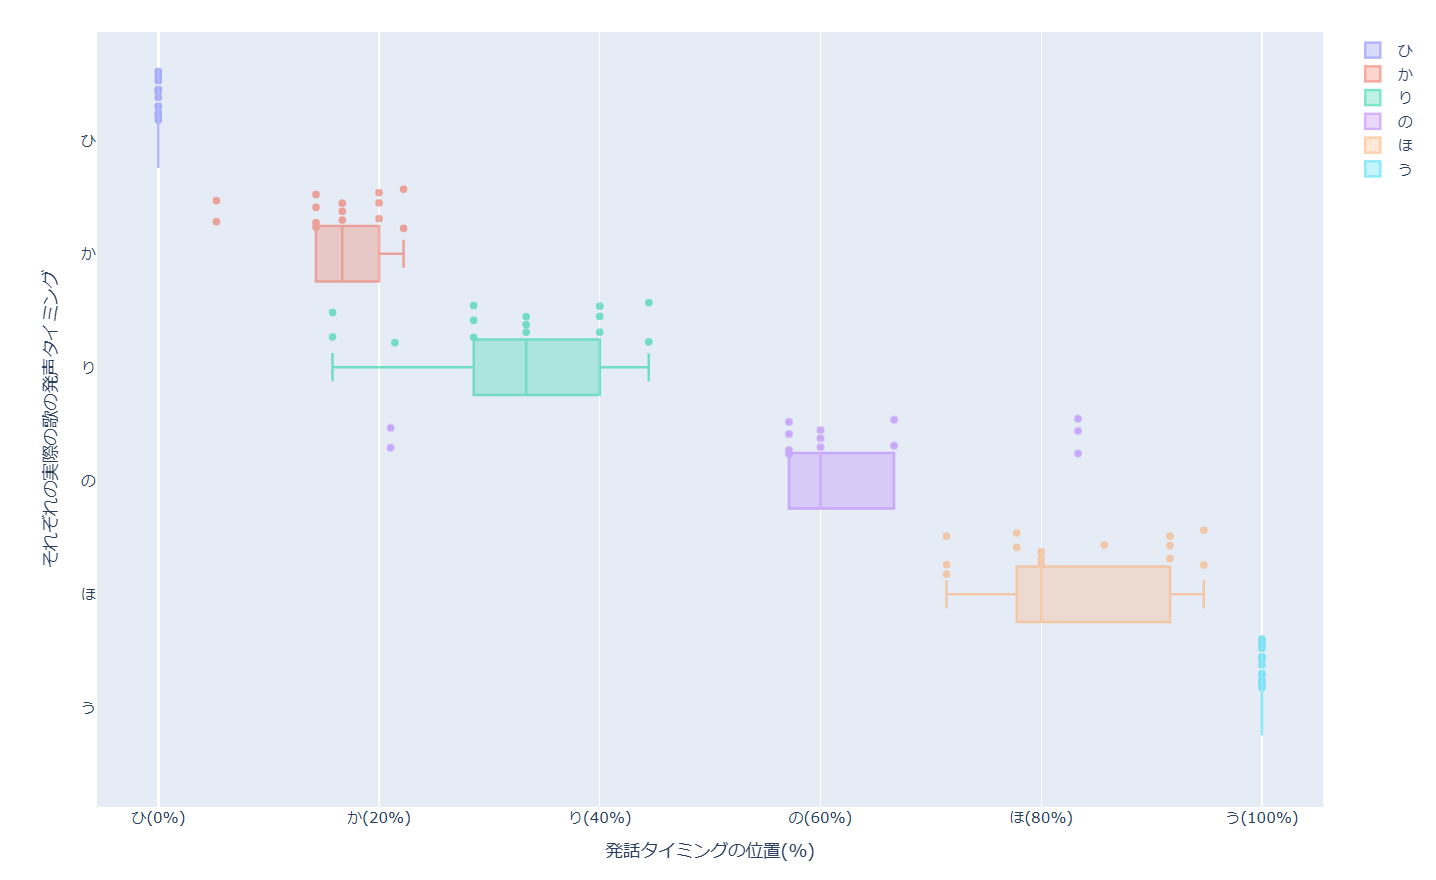
\includegraphics[width=\columnwidth]{fig/hikari/kongo/tai.png}
    \subcaption{混合でのタイミングの違い}
    \label{h_kongo_tai}
  \end{minipage}
  \begin{minipage}{0.3\hsize}
    \centering
    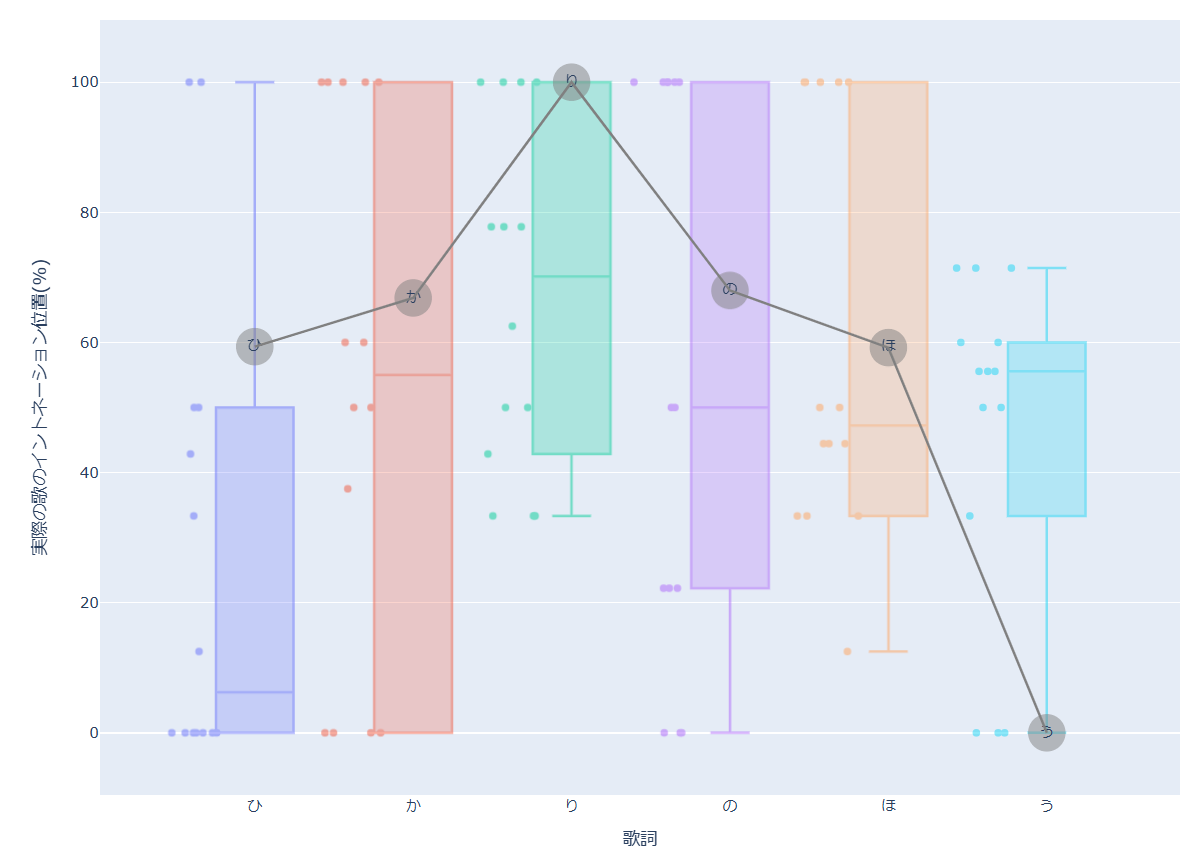
\includegraphics[width=\columnwidth]{fig/hikari/kongo/int.png}
    \subcaption{混合でのイントネーションの違い}
    \label{h_kongo_int}
  \end{minipage}
  \begin{minipage}{0.3\hsize}
    \centering
    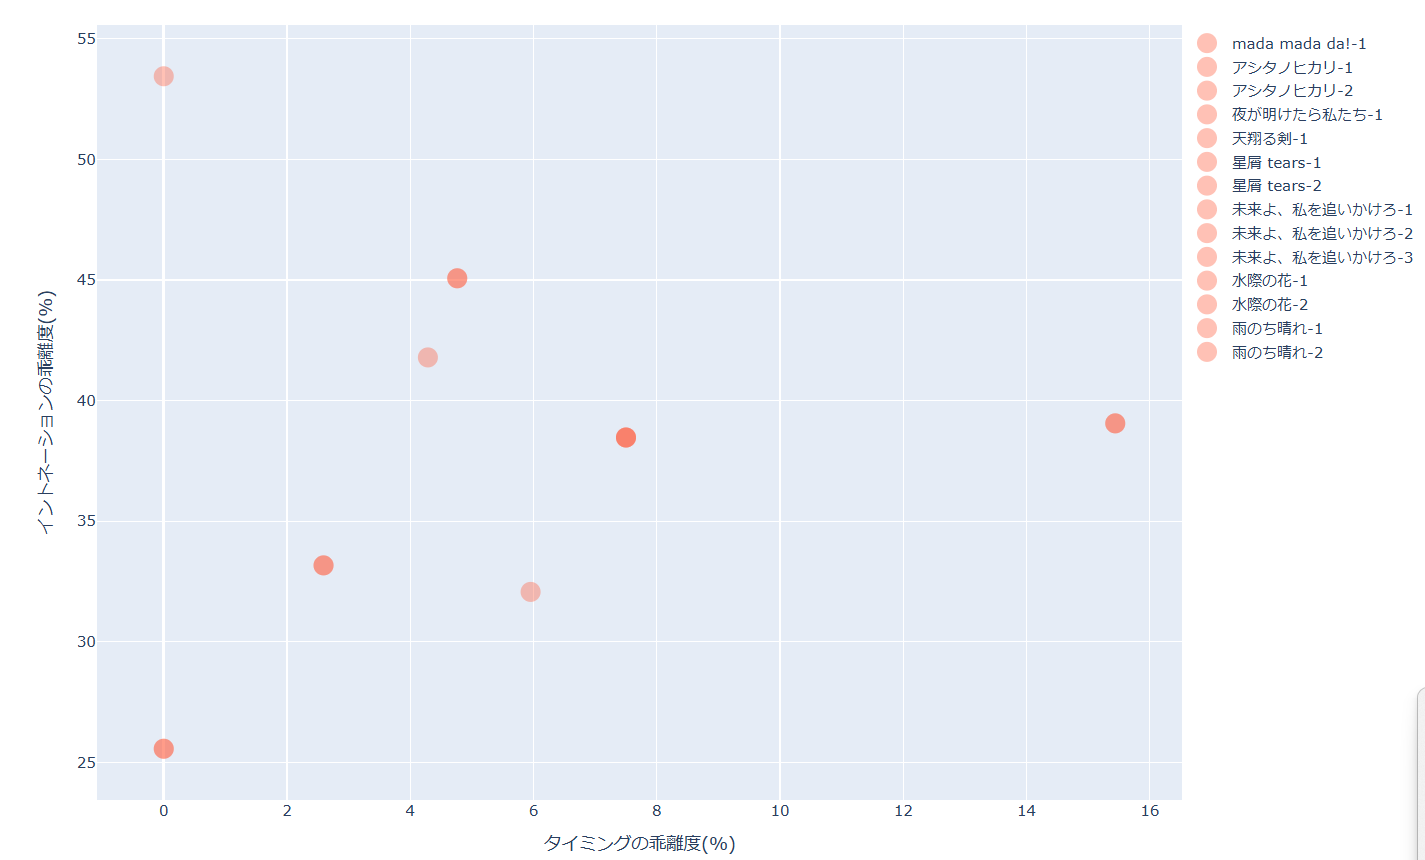
\includegraphics[width=\columnwidth]{fig/hikari/kongo/tai_int.png}
    \subcaption{混合でのタイミングとイントネーションの乖離}
    \label{h_kongo_tai_int}
  \end{minipage}
  \caption{「ひかりのほう」の混合での発話表現との比較}
  \label{h_kongo_hakohige}
\end{figure*}

\begin{figure*}[t]
  \centering
  \begin{minipage}{0.49\hsize}
    \centering
    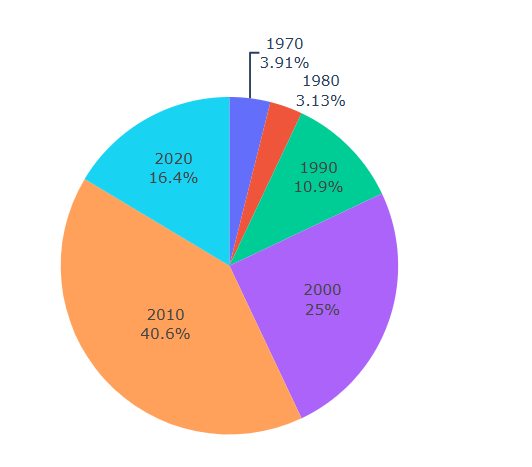
\includegraphics[width=\columnwidth]{fig/anata/nendai_wariai.png}
    \subcaption{“あなたにあいたくて”}
    \label{a_nendai_wari}
  \end{minipage}
  \begin{minipage}{0.49\hsize}
    \centering
    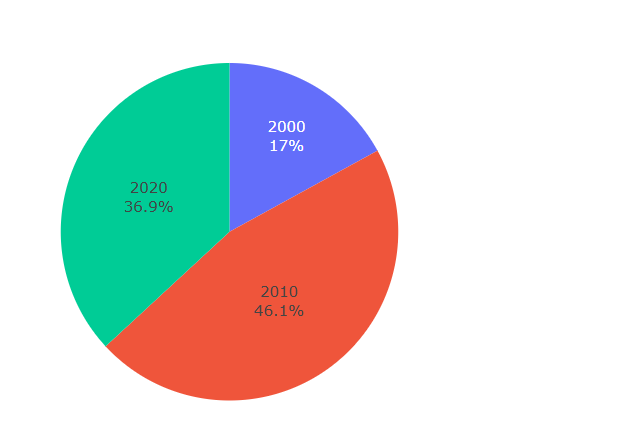
\includegraphics[width=\columnwidth]{fig/hikari/nendai_wariai.png}
    \subcaption{“ひかりのほう”}
    \label{h_nendai_wari}
  \end{minipage}
  \caption{年代ごとの割合}
  \label{nendai_wari}
\end{figure*}

\begin{figure*}[t]
  \centering
  \begin{minipage}{0.3\hsize}
    \centering
    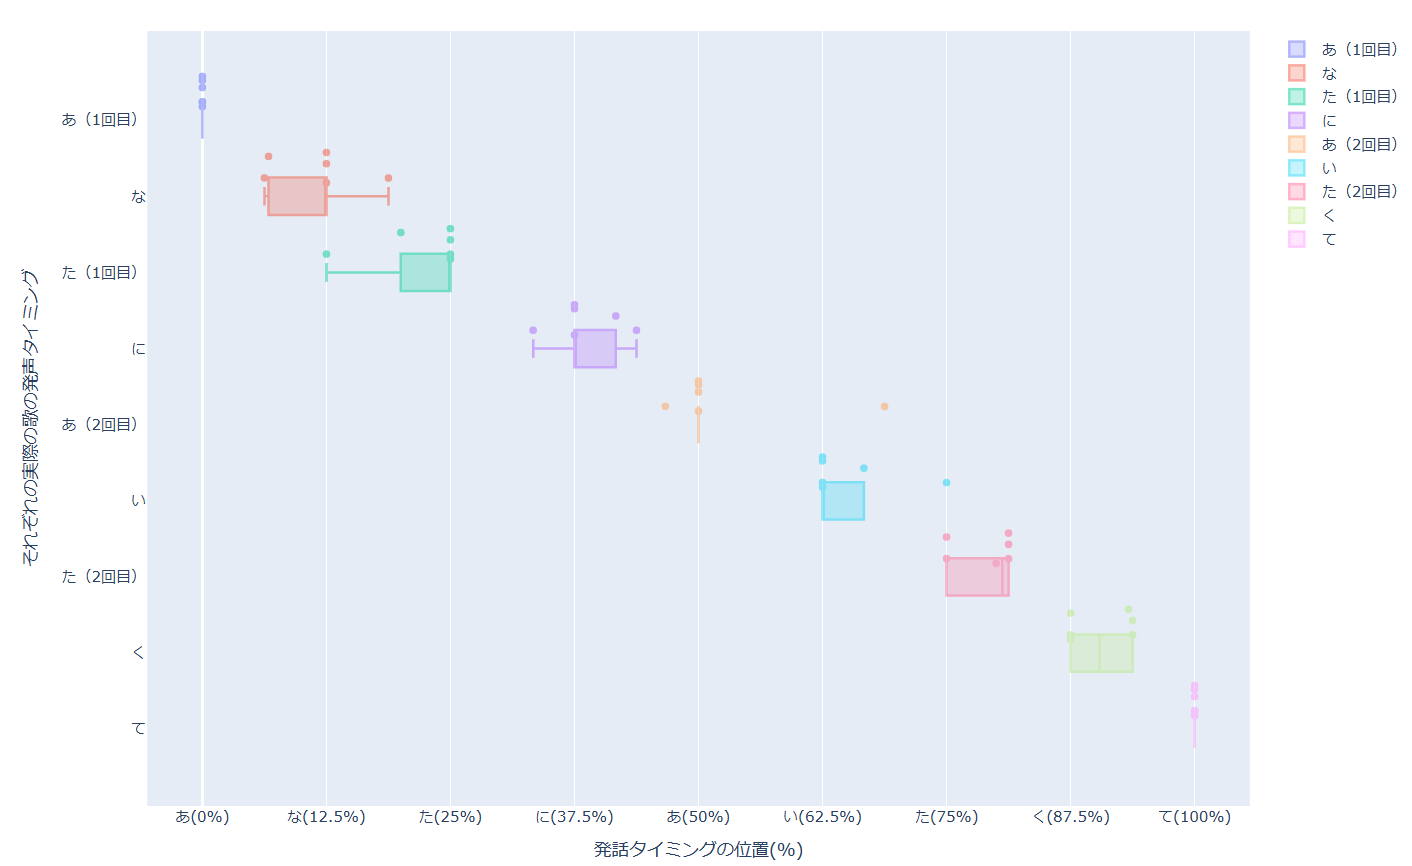
\includegraphics[width=\columnwidth]{fig/anata/1970/tai.png}
    \subcaption{1970年代でのタイミングの違い}
    \label{1970_tai}
  \end{minipage}
  \begin{minipage}{0.3\hsize}
    \centering
    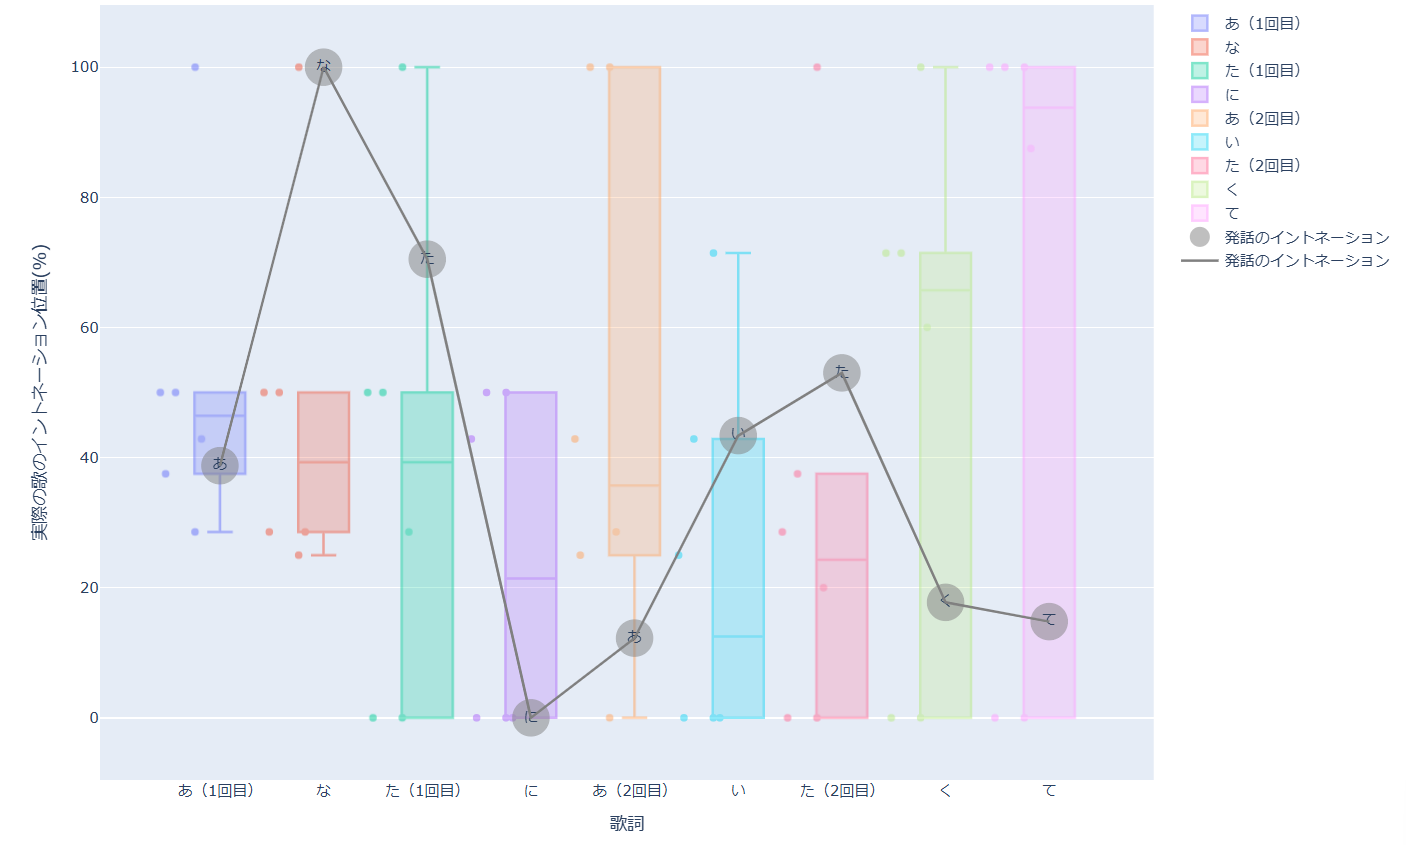
\includegraphics[width=\columnwidth]{fig/anata/1970/int.png}
    \subcaption{1970年代でのイントネーションの違い}
    \label{1970_int}
  \end{minipage}
  \begin{minipage}{0.3\hsize}
    \centering
    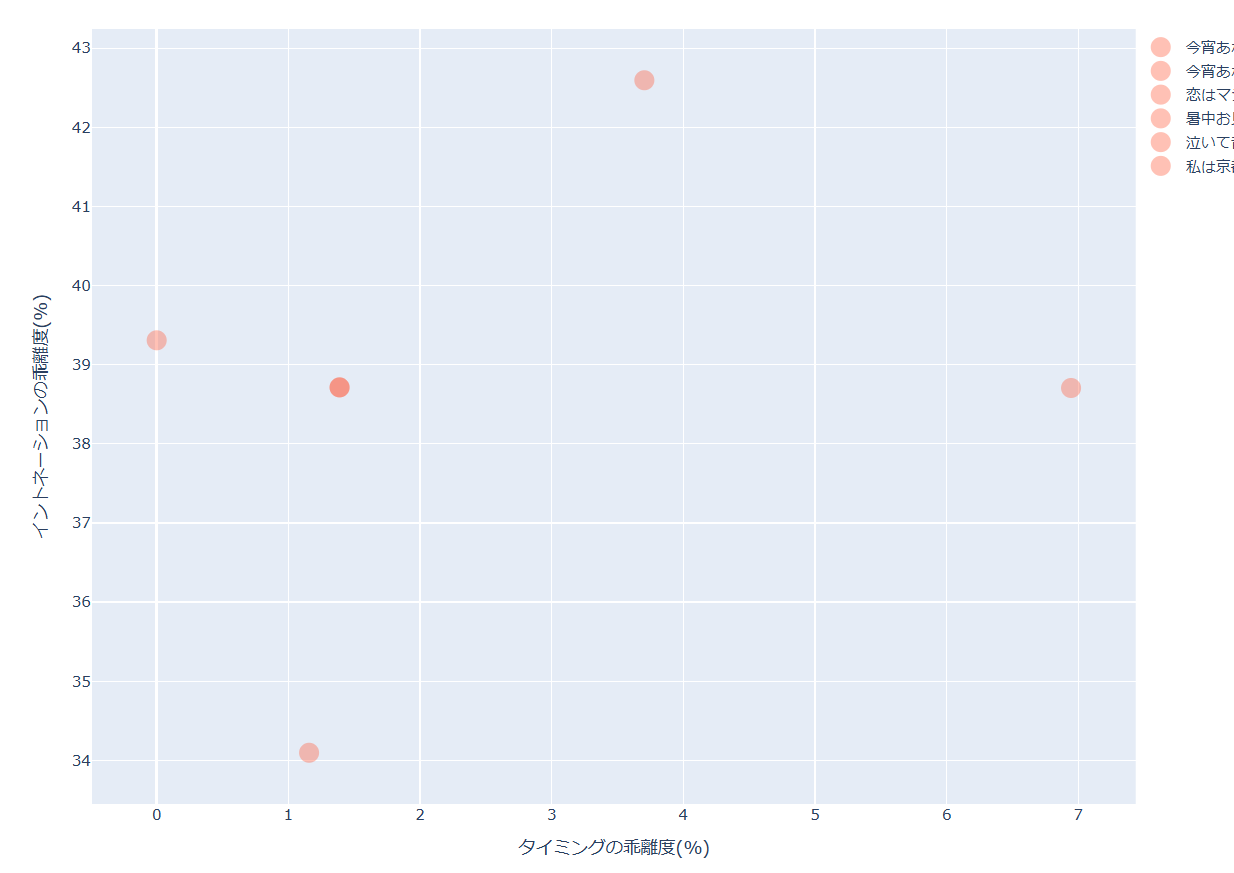
\includegraphics[width=\columnwidth]{fig/anata/1970/tai_int.png}
    \subcaption{1970年代でのタイミングとイントネーションの乖離}
    \label{1970_tai_int}
  \end{minipage}
  \caption{「あなたにあいたくて」の1970年代での発話表現との比較}
  \label{1970_hakohige}
\end{figure*}




\begin{figure*}[t]
  \centering
  \begin{minipage}{0.3\hsize}
    \centering
    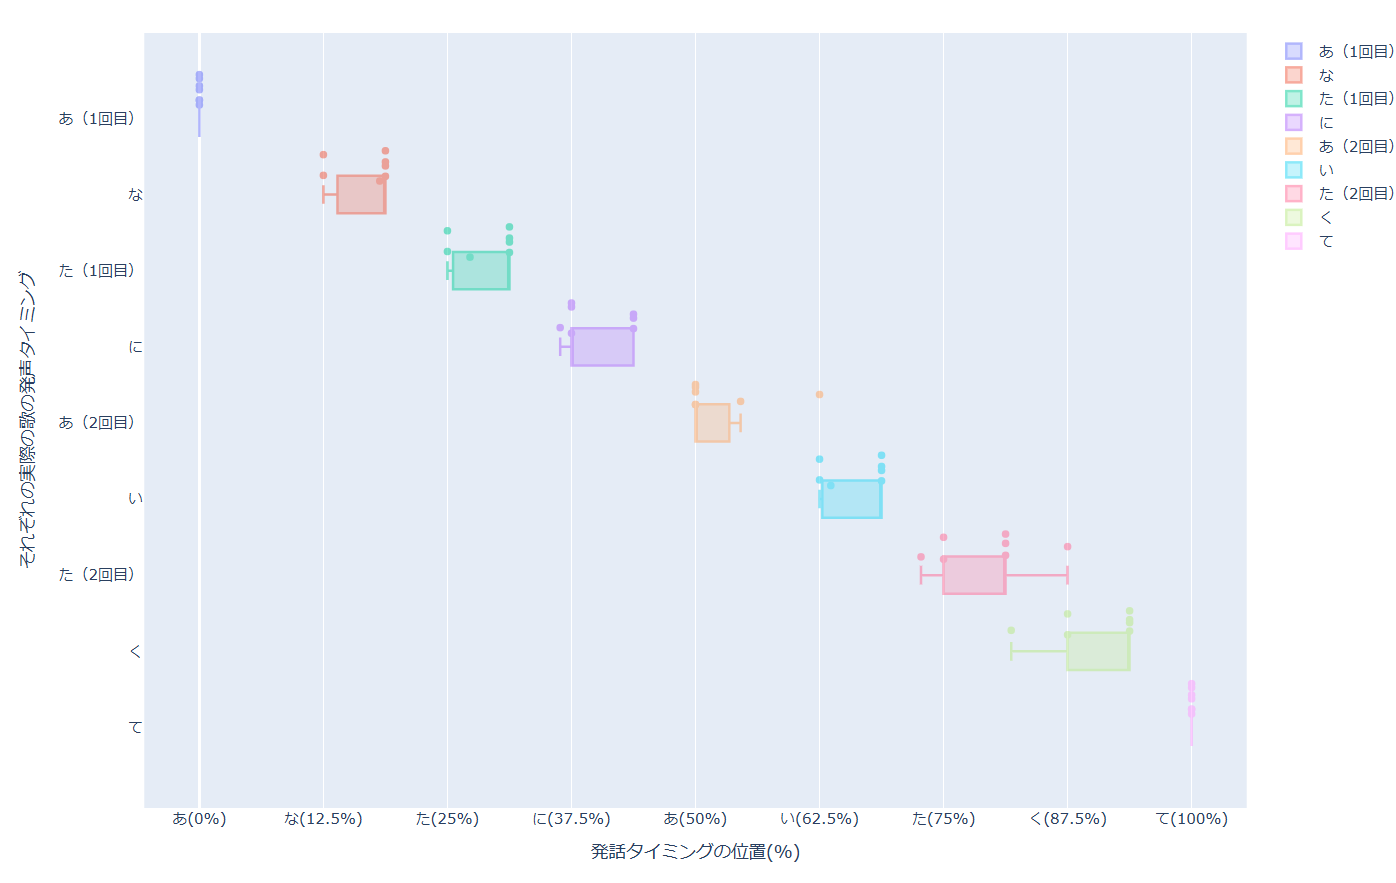
\includegraphics[width=\columnwidth]{fig/anata/1980/tai.png}
    \subcaption{1980年代でのタイミングの違い}
    \label{1980_tai}
  \end{minipage}
  \begin{minipage}{0.3\hsize}
    \centering
    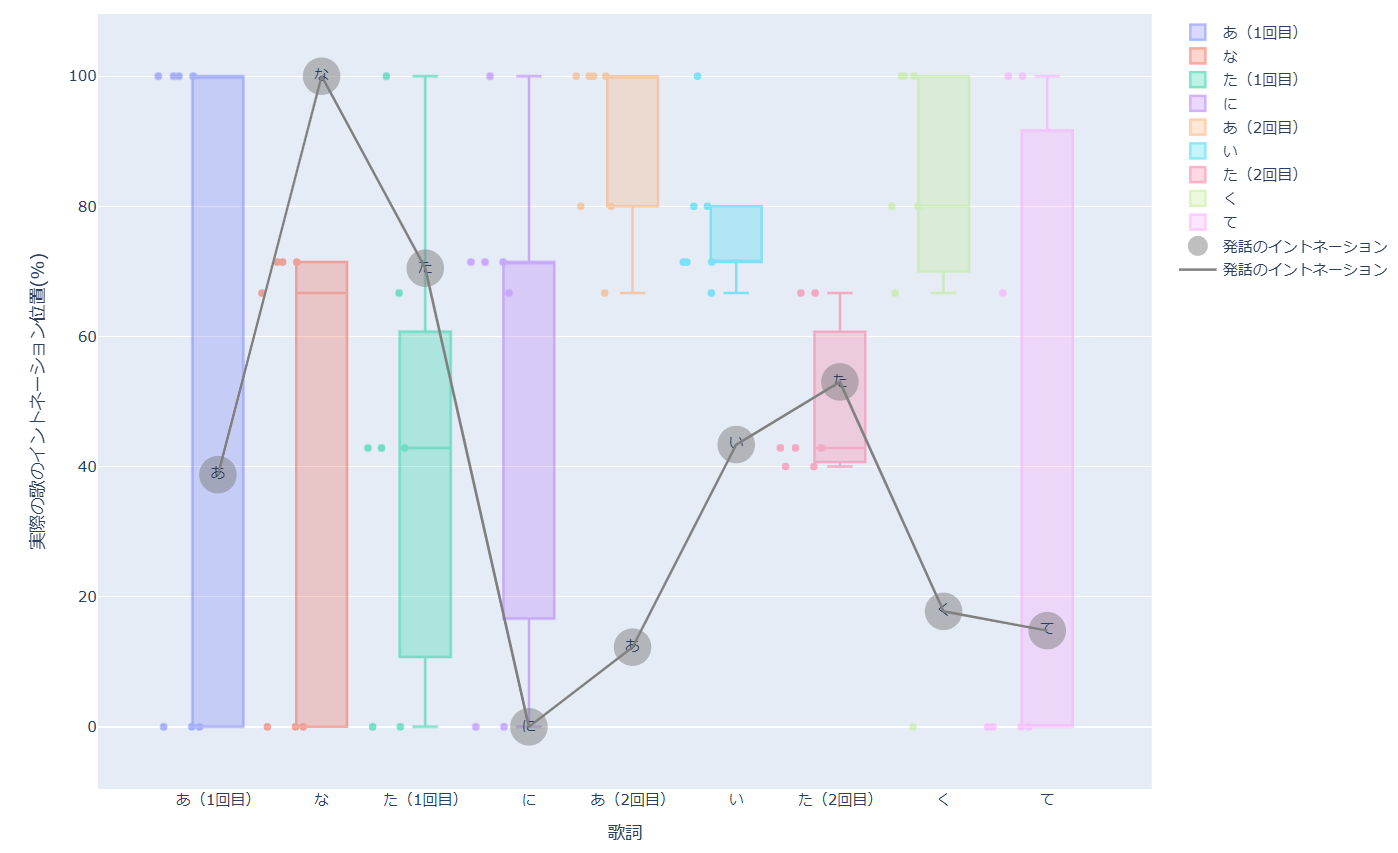
\includegraphics[width=\columnwidth]{fig/anata/1980/int.png}
    \subcaption{1980年代でのイントネーションの違い}
    \label{1980_int}
  \end{minipage}
  \begin{minipage}{0.3\hsize}
    \centering
    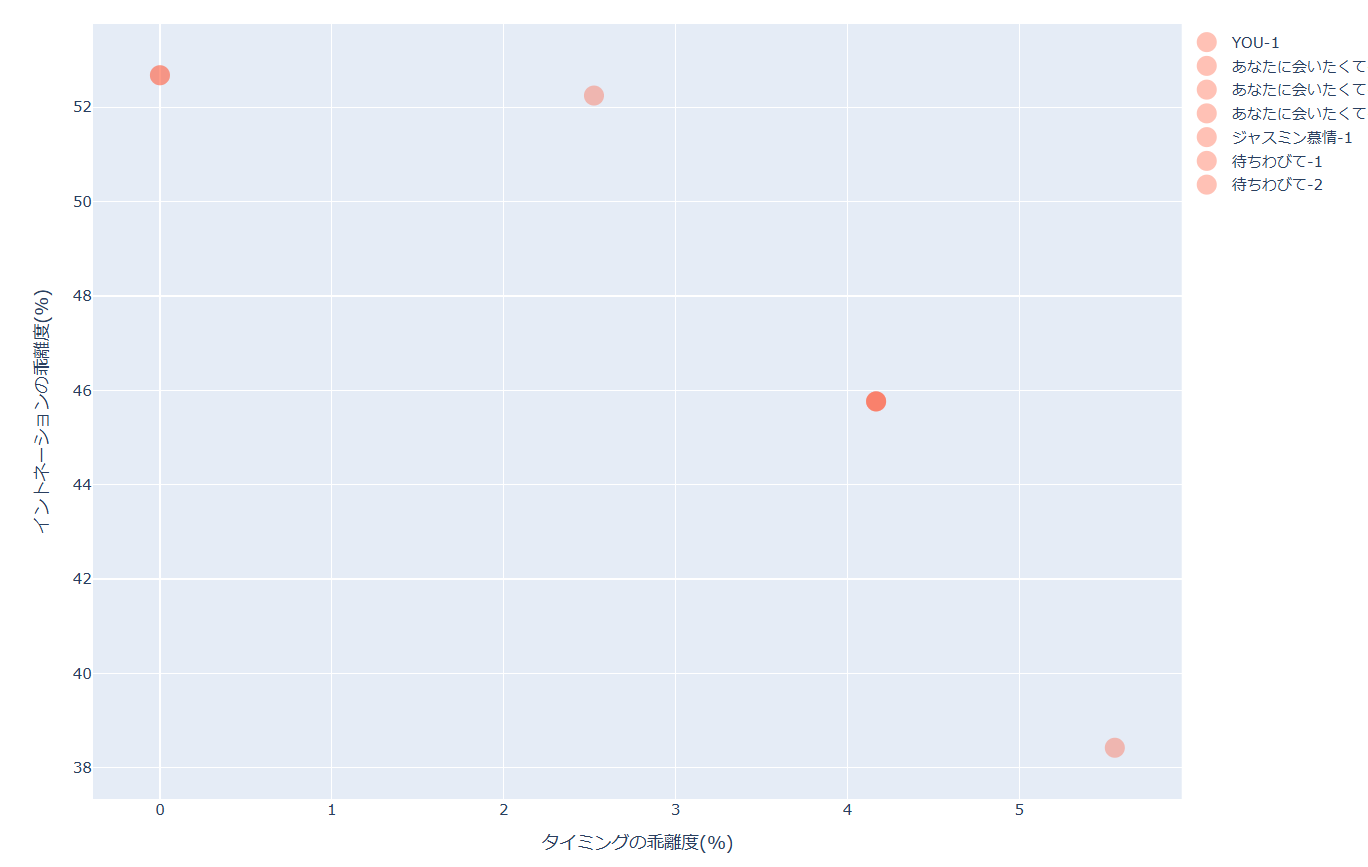
\includegraphics[width=\columnwidth]{fig/anata/1980/tai_int.png}
    \subcaption{1980年代でのタイミングとイントネーションの乖離}
    \label{1980_tai_int}
  \end{minipage}
  \caption{「あなたにあいたくて」の1980年代での発話表現との比較}
  \label{1980_hakohige}
\end{figure*}


\begin{figure*}[t]
  \centering
  \begin{minipage}{0.3\hsize}
    \centering
    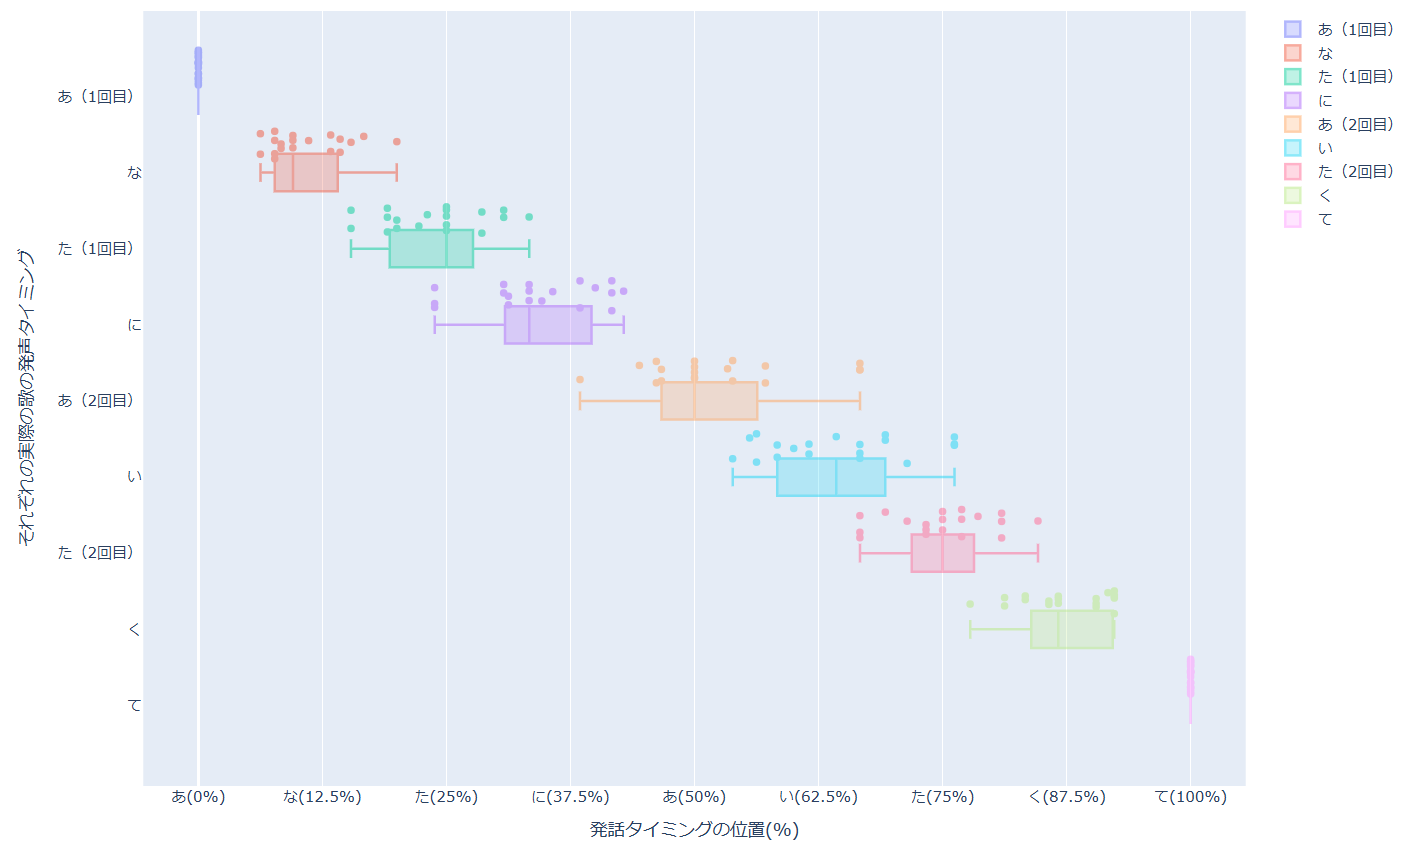
\includegraphics[width=\columnwidth]{fig/anata/1990/tai.png}
    \subcaption{1990年代でのタイミングの違い}
    \label{1990_tai}
  \end{minipage}
  \begin{minipage}{0.3\hsize}
    \centering
    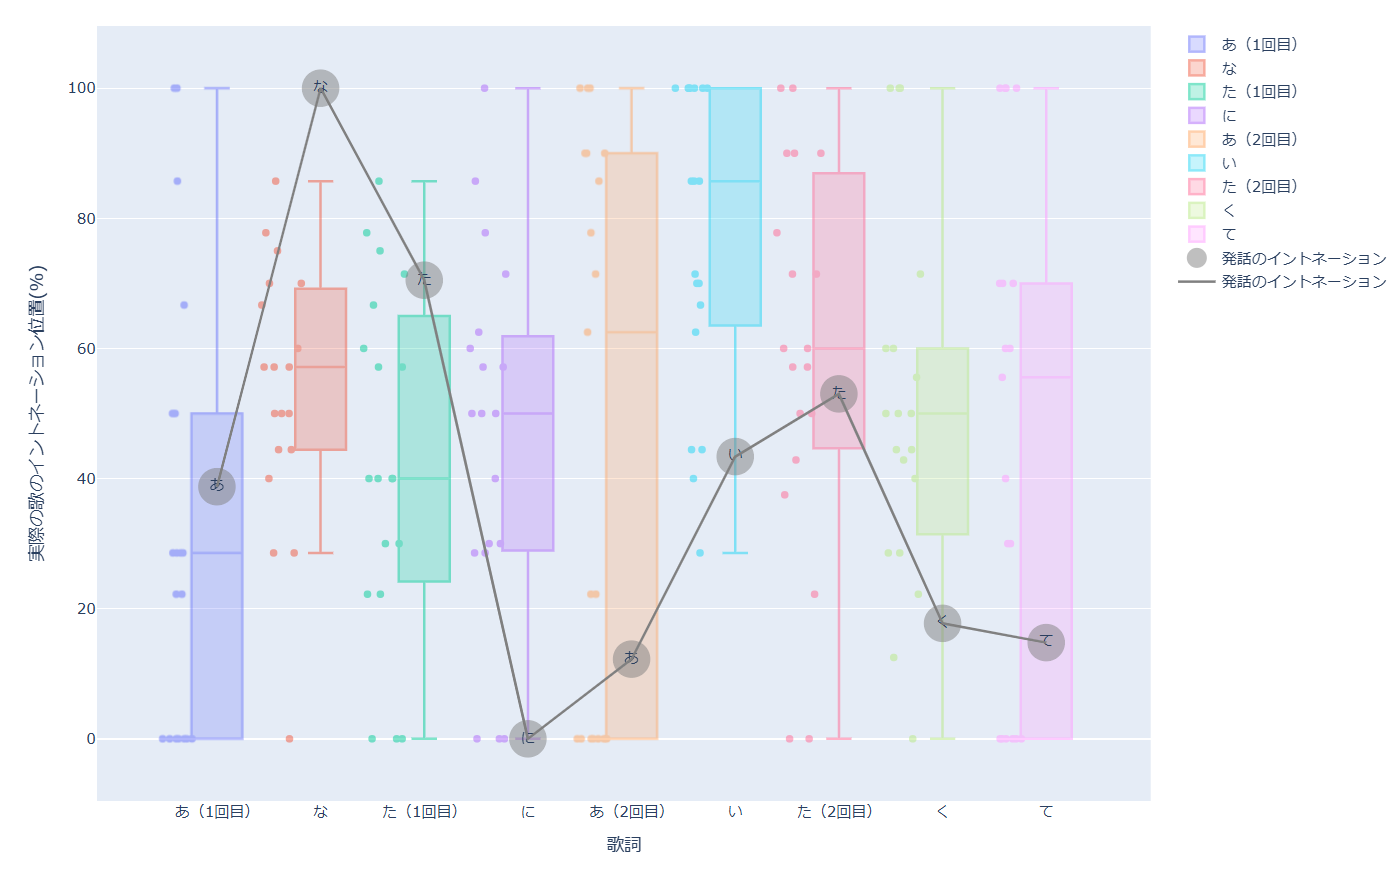
\includegraphics[width=\columnwidth]{fig/anata/1990/int.png}
    \subcaption{1990年代でのイントネーションの違い}
    \label{1990_int}
  \end{minipage}
  \begin{minipage}{0.3\hsize}
    \centering
    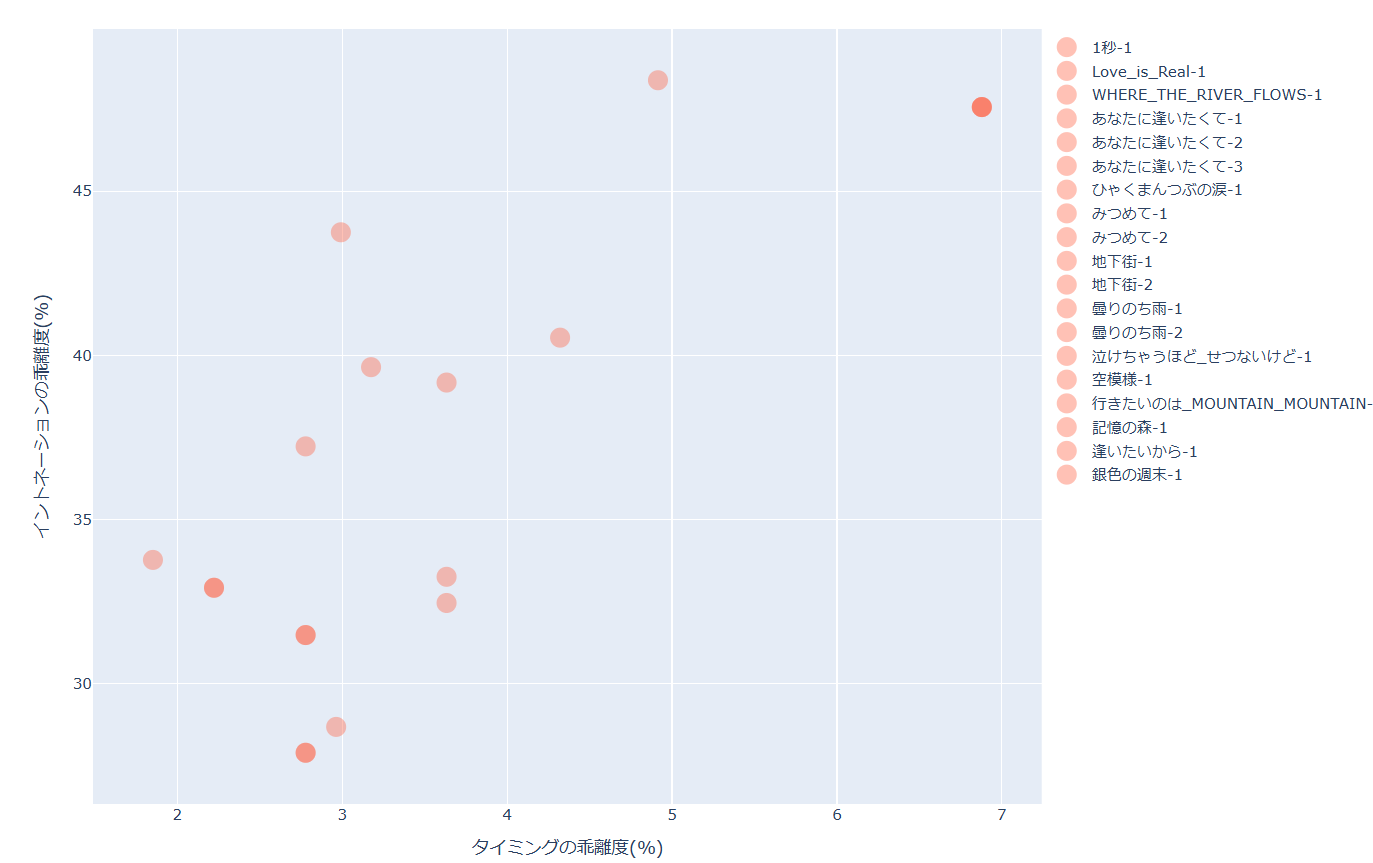
\includegraphics[width=\columnwidth]{fig/anata/1990/tai_int.png}
    \subcaption{1990年代でのタイミングとイントネーションの乖離}
    \label{1990_tai_int}
  \end{minipage}
  \caption{「あなたにあいたくて」の1990年代での発話表現との比較}
  \label{1990_hakohige}
\end{figure*}










\textbf{“ひかりのほう”での結果}\par
%デュエットなど，男女混合で歌っているものをプロットしたのが\figref{h_kongo}である．\par
%音長は8拍以内で歌われている．また，音の高さはMIDIナンバーで53～73，つまりF3～C\(\sharp \)5の間で歌われており，女性と男性の平均音域を合わせたものよりも狭くなっている．
\figref{h_kongo_tai}より，「か」「り」のみ中央値とタイミングの不一致が起こっている．また，「か」と「り」において，第三四分位数と発話タイミングが一致していることから，75\%のフレーズが発話タイミングと同じか早く発音されている．また，「の」において，2つ前の単音の発話タイミングの位置付近まで外れ値があることがわかる．\par
また，\figref{h_kongo_int}において，「り」「の」「ほ」「う」において，最大値および第一四分位数が100にあることから，各単音の最低でも4分の1がフレーズ内の最も高い音で歌われていることがわかる．\par
また，「ひ」「か」「う」において，最小値および第三四分位数が0の位置にあることから，各単音の少なくとも4分の1がフレーズ内の最も低い音で歌われていることがわかる．さらに「ひ」については，中央値も0の位置にあることから，少なくとも半分の楽曲がフレーズ内の最も低い音で歌われていることがわかる．\par
さらに，\figref{h_kongo_tai_int}において，イントネーションの乖離度は0\%から75\%付近までばらつきがあり，タイミングの乖離度は0\%付近から15\%ほどであるとわかる．また，\ref{sec:4.3.3}と同じく，タイミングの乖離度が0\%の位置，つまり発話タイミングと同じタイミングで歌われている楽曲が固まっていることがわかる．


%4.4
\subsection{年代別の割合}
“あなたにあいたくて”“ひかりのほう”それぞれの発表年代ごとの割合が\figref{a_nendai_wari}，\figref{h_nendai_wari}である．


“あなたにあいたくて”について，\figref{a_nendai_wari}により，2010年代が一番多く，その次に2000年代が多いことがわかる．\par
また，“ひかりのほう”について，\figref{h_nendai_wari}により，20世紀に発表された楽曲が全くなく，「ひかりのほう」は2000年代から使われ始めていることがわかる．
次項から，各フレーズにおいて年代ごとの発話表現との一致度について記していく


%4.4.1
\subsubsection{1970年代のグラフ}


\textbf{“あなたにあいたくて”での結果}\par
%1970年代のグラフは\figref{a_nendai_1970}である．グラフより，1970年代は「あなたにあいたくて」は長くとも12拍で歌い切られていることがわかる．また，最高音は71，最低音は54であった．\par
\figref{1970_tai}より，「あ（2回目）」において，ほとんど発話タイミングと同じ位置で歌われていることがわかる．また，他の単音においても，かなり発話タイミングと近い位置で歌われていることがわかる．\par
また，\figref{1970_int}において，「あ（1回目）」「な」において，イントネーション位置が50\%の位置に近いところに固まっていることがわかる．また，「た（1回目)」「に」「い」「た（2回目）」「く」「て」において最小値および第一四分位数が0\%の位置にあることから，各単音の少なくとも4分の1がフレーズ内の最も低い音で歌われていることがわかる．また，「あ（2回目）」「て」において，最大値および第三四分位数が100\%の位置にあることから，少なくとも4分の1がフレーズ内の最も高い音で歌われていることがわかる．\par
さらに，\figref{1970_tai_int}において，イントネーションの乖離度は34\%から43\%付近でまとまっており，タイミングの乖離度は0\%付近から7\%ほどであるとわかる．


\textbf{“ひかりのほう”での結果}\par
“ひかりのほう”フレーズにおいて，1970年代に発表された楽曲は存在しない．

%4.4.2
\subsubsection{1980年代のグラフ}

\textbf{“あなたにあいたくて”での結果}\par
%1980年代のグラフは\figref{a_nendai_1980}である．グラフより，1980年代は「あなたにあいたくて」は長くとも14拍で歌い切られていることがわかる．また，最高音は70，最低音は62であった．\par
\figref{1980_tai}より，すべての単音において，第一四分位数および最小値が発話タイミングと一致，もしくは限りなく近いことから，ほとんど全てのフレーズは発話タイミングと同じか遅く発音されていることがわかる．\par
また，\figref{1980_int}において，「あ（1回目）」「て」において，中央値が100\%および0\%にあり，また第一四分位数が0で第三四分位数が100\%の位置にあるため，この2つに関してはフレーズ内の最も高い音か最も低い音で歌われることが多いことがわかる．また，「あ（2回目）」と「い」，「く」において，約65\%の位置から高いイントネーション位置にしか存在しないことがわかる．また，「た（2回目）」において，40\%から65\%と，狭い範囲で固まっていることがわかる．
さらに，\figref{1980_tai_int}において，イントネーションの乖離度は約38\%から52\%付近となっており，タイミングの乖離度は0\%から6\%付近ほどであるとわかる．


\textbf{“ひかりのほう”での結果}\par
“ひかりのほう”フレーズにおいて，1980年代に発表された楽曲は存在しない．


%4.4.3
\subsubsection{1990年代のグラフ}

\textbf{“あなたにあいたくて”での結果}\par
%1990年代のグラフは\figref{a_nendai_1990}である．グラフより，1990年代は「あなたにあいたくて」は長くとも16拍で歌い切られていることがわかる．また，最高音は74，最低音は49であった．\par
\figref{1990_tai}より，「た（1回目）」「あ（2回目）」「た（2回目）」において，中央値が一致していることがわかる．\par
また，\figref{1990_int}において，「あ（1回目）」「あ（2回目）」「て」において，最小値および第一四分位数が0\%の位置にあることから，各単音の少なくとも4分の1がフレーズ内の最も低い音で歌われていることがわかる．また，「い」において，最大値および第三四分位数が100\%の位置にあることから，少なくとも4分の1がフレーズ内の最も高い音で歌われていることがわかる．\par
さらに，\figref{1990_tai_int}において，イントネーションの乖離度は0\%から58\%付近までばらつきがあり，タイミングの乖離度は0\%付近から13\%ほどであるとわかる．


\textbf{“ひかりのほう”での結果}\par
“ひかりのほう”フレーズにおいて，1990年代に発表された楽曲は存在しない．


\begin{figure*}[t]
  \centering
  \begin{minipage}{0.3\hsize}
    \centering
    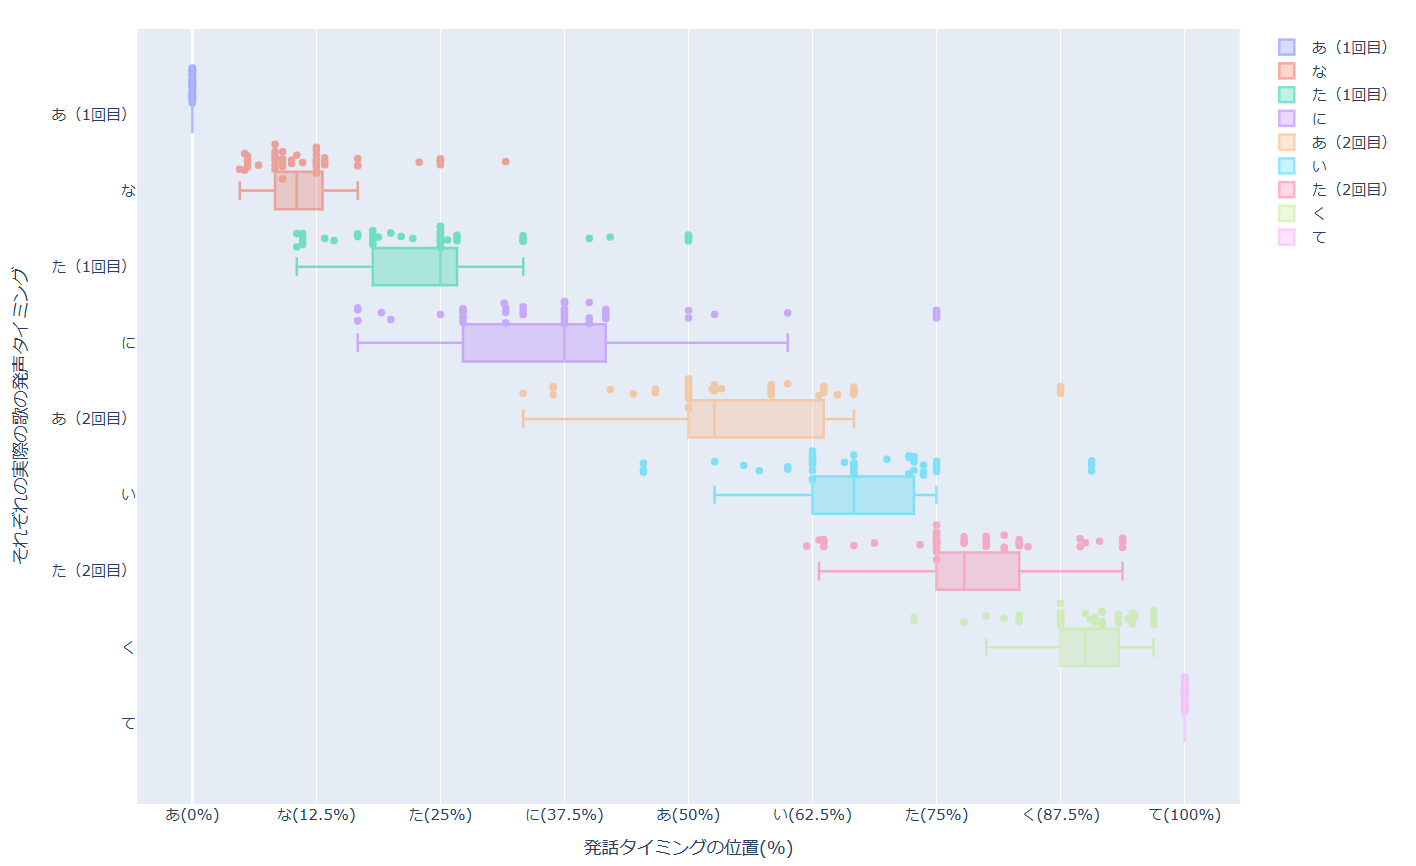
\includegraphics[width=\columnwidth]{fig/anata/2000/tai.png}
    \subcaption{2000年代でのタイミングの違い}
    \label{a_2000_tai}
  \end{minipage}
  \begin{minipage}{0.3\hsize}
    \centering
    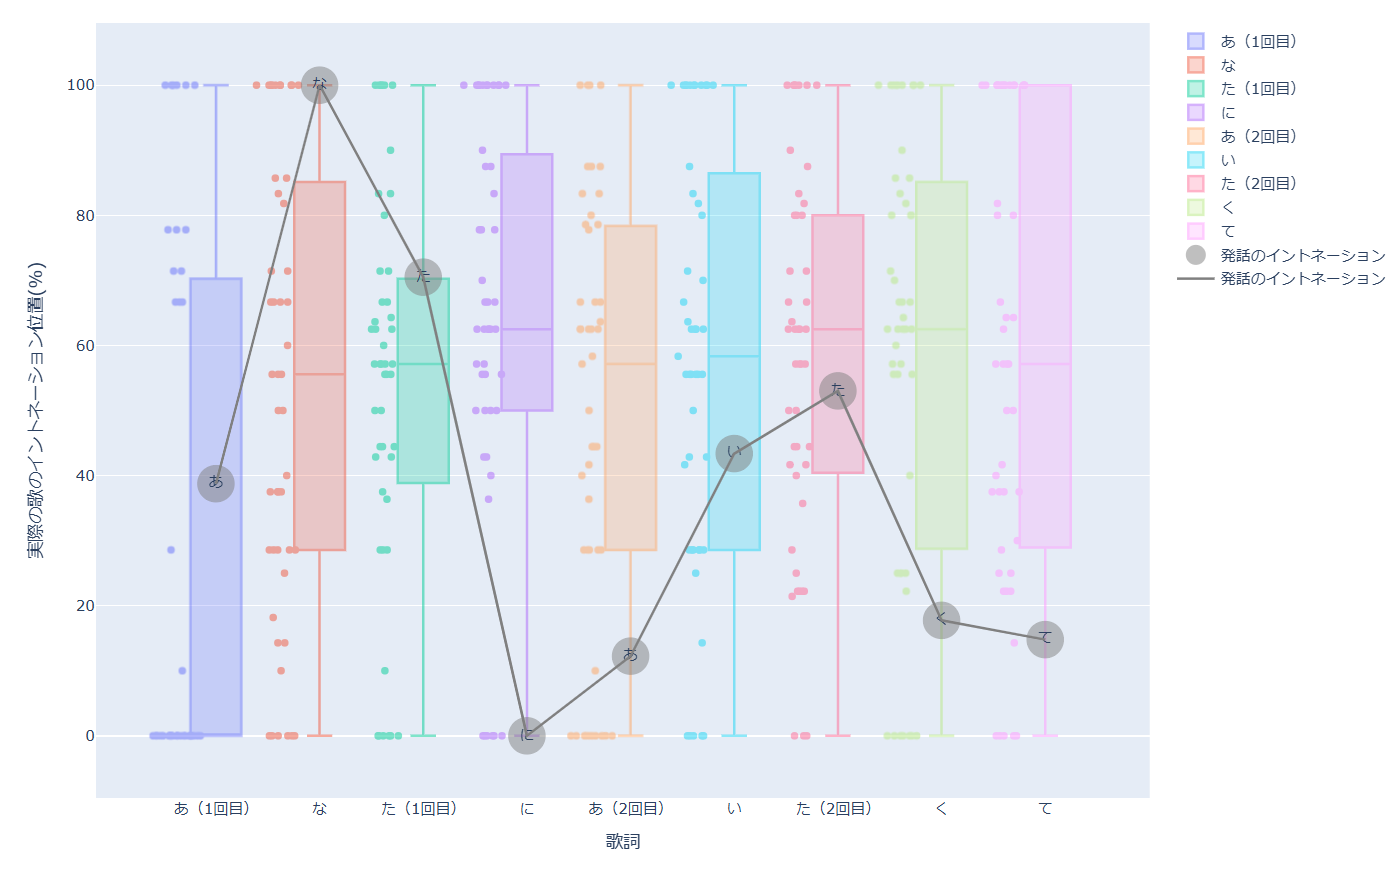
\includegraphics[width=\columnwidth]{fig/anata/2000/int.png}
    \subcaption{2000年代でのイントネーションの違い}
    \label{a_2000_int}
  \end{minipage}
  \begin{minipage}{0.3\hsize}
    \centering
    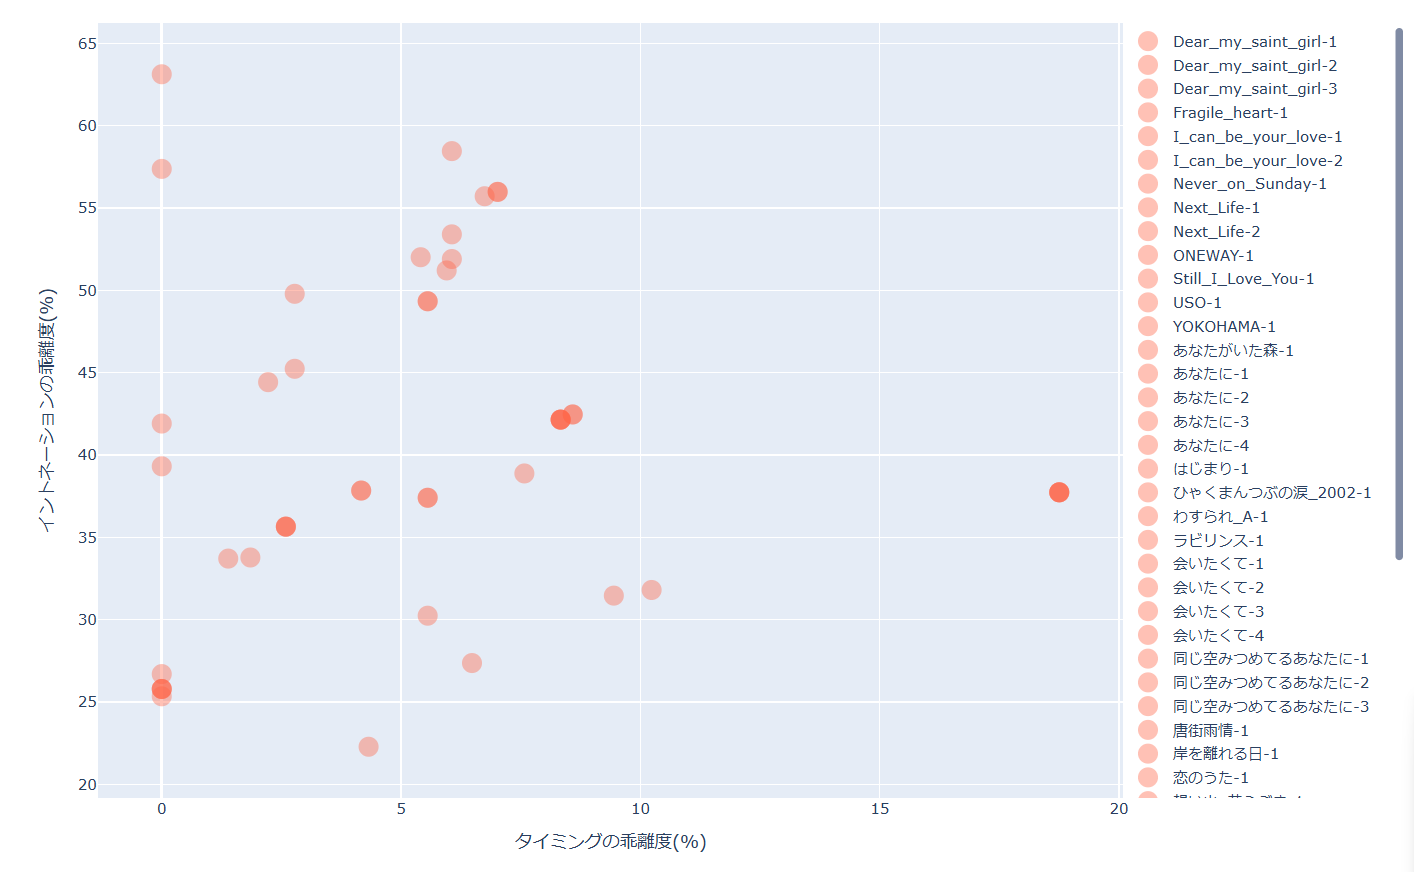
\includegraphics[width=\columnwidth]{fig/anata/2000/tai_int.png}
    \subcaption{2000年代でのタイミングとイントネーションの乖離}
    \label{a_2000_tai_int}
  \end{minipage}
  \caption{「あなたにあいたくて」の2000年代での発話表現との比較}
  \label{a_2000_hakohige}
\end{figure*}
\begin{figure*}[t]
  \centering
  \begin{minipage}{0.3\hsize}
    \centering
    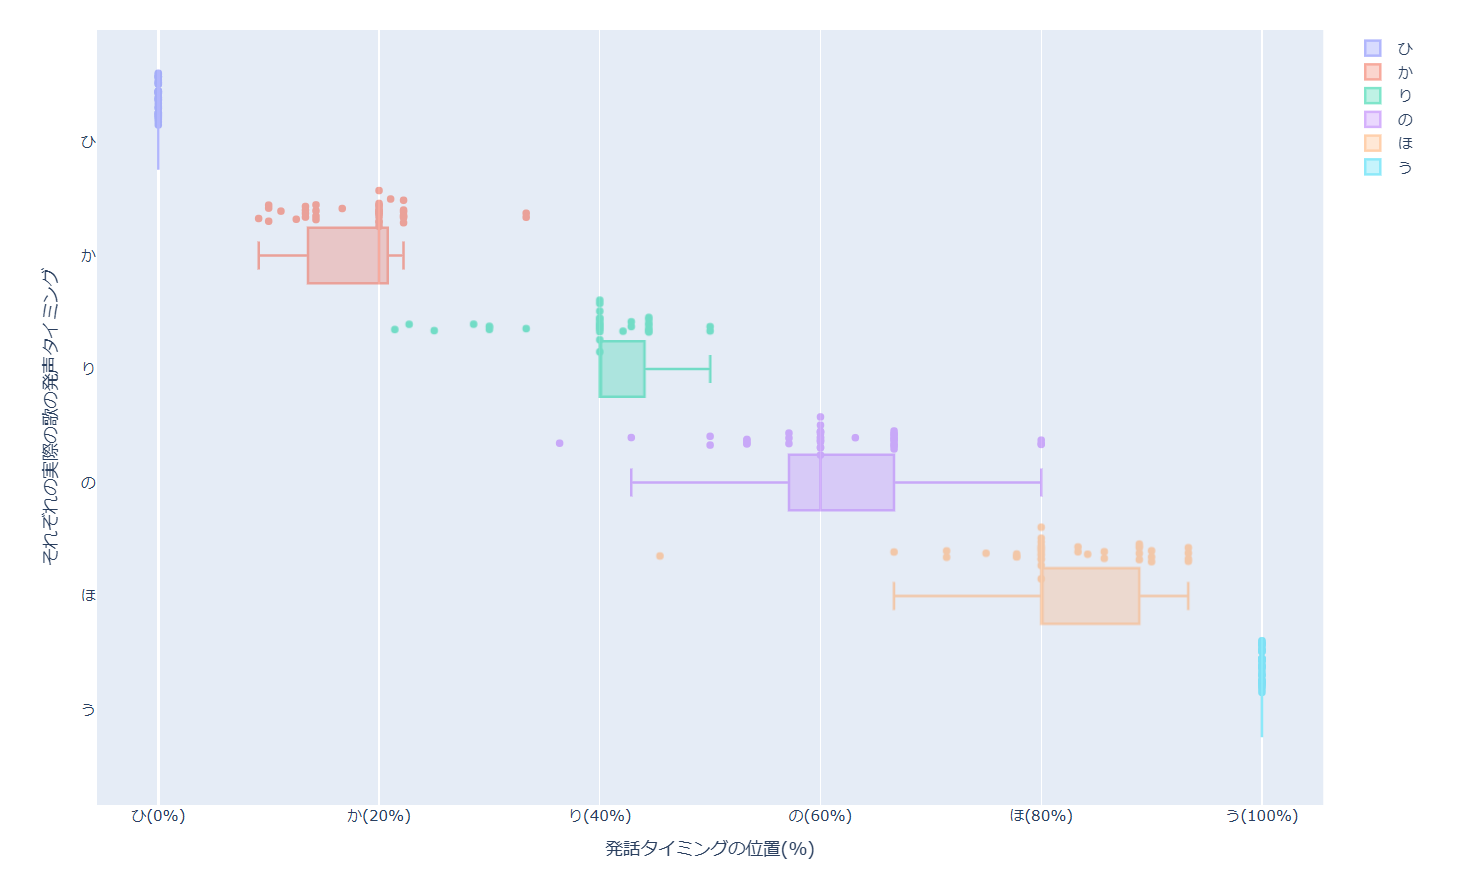
\includegraphics[width=\columnwidth]{fig/hikari/2000/tai.png}
    \subcaption{2000年代でのタイミングの違い}
    \label{h_2000_tai}
  \end{minipage}
  \begin{minipage}{0.3\hsize}
    \centering
    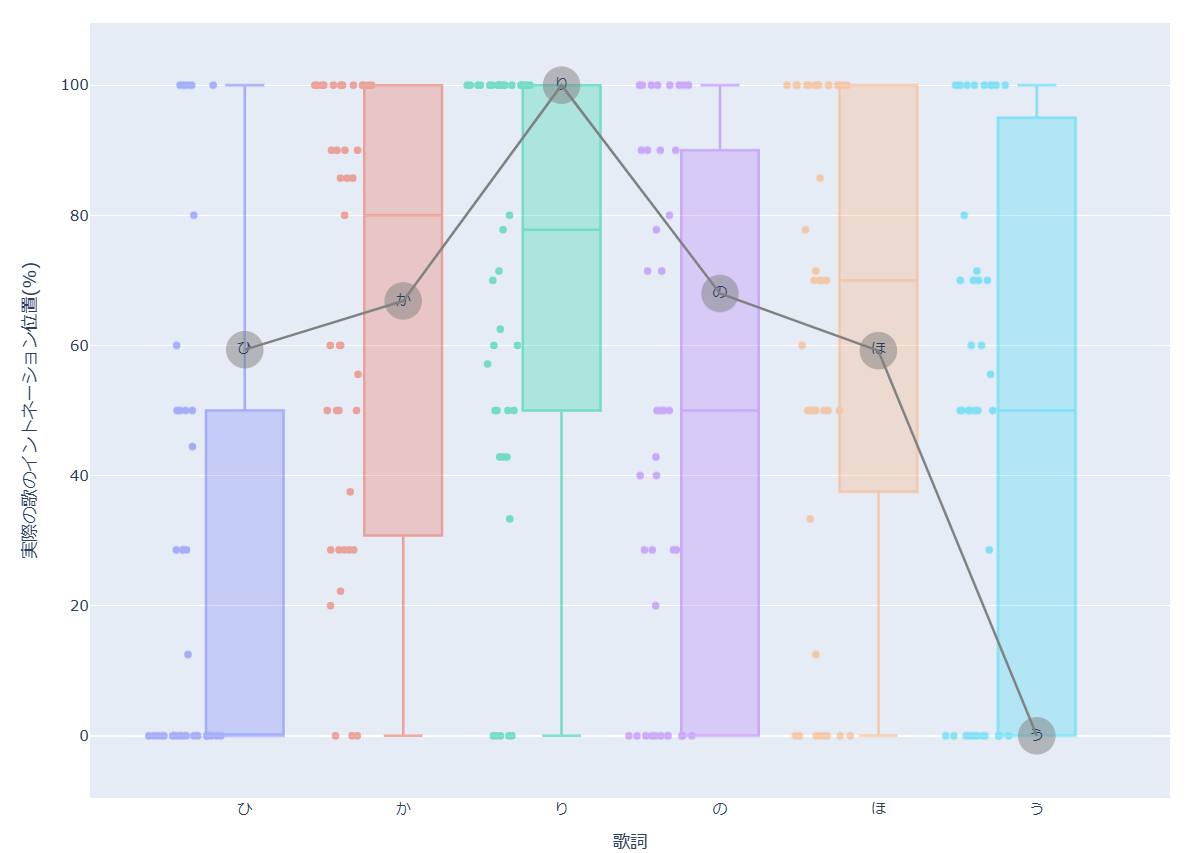
\includegraphics[width=\columnwidth]{fig/hikari/2000/int.png}
    \subcaption{2000年代でのイントネーションの違い}
    \label{h_2000_int}
  \end{minipage}
  \begin{minipage}{0.3\hsize}
    \centering
    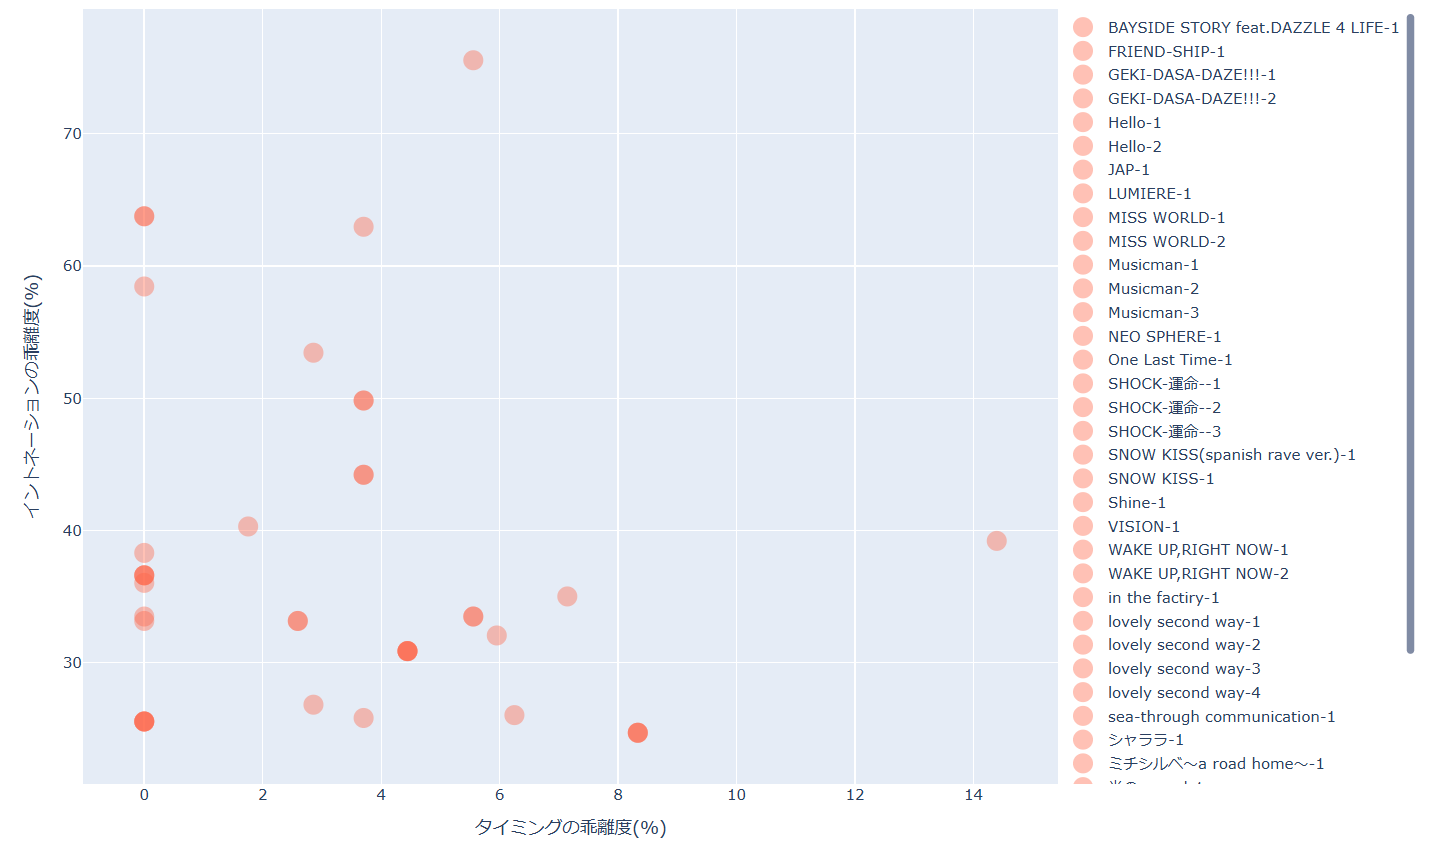
\includegraphics[width=\columnwidth]{fig/hikari/2000/tai_int.png}
    \subcaption{2000年代でのタイミングとイントネーションの乖離}
    \label{h_2000_tai_int}
  \end{minipage}
  \caption{「ひかりのほう」の2000年代での発話表現との比較}
  \label{h_2000_hakohige}
\end{figure*}

%4.4.4
\subsubsection{2000年代のグラフ}

\textbf{“あなたにあいたくて”での結果}\par
%2000年代のグラフは\figref{a_nendai_2000}である．グラフより，2000年代は「あなたにあいたくて」は長くとも22拍で歌い切られていることがわかる．また，最高音は73，最低音は45であった．\par
\figref{a_2000_tai}より，「た（1回目）」「に」において，中央値が発話タイミングと一致していることがわかる．また，「あ」「い」「た（2回目）」「く」において，第一四分位数発話タイミングと一致することから，75\%が発話タイミングと同じか遅く発音されている．\par
また，\figref{a_2000_int}より，「あ（1回目）」において，第三四分位数が0\%の位置にあることから，少なくとも4分の1が最も低い音で歌われていることがわかる．また，「て」について，最大値および第一四分位数が100\%にあることから，各単音の最低でも4分の1がフレーズ内の最も高い音で歌われていることがわかる．\par
さらに，\figref{a_2000_tai_int}において，イントネーションの乖離度は22\%から63\%となっており，タイミングの乖離度は0\%から20\%ほどであるとわかる．


\textbf{“ひかりのほう”での結果}\par
%2000年代のグラフは\figref{h_nendai_2000}である．グラフより，2000年代は「ひかりのほう」は長くとも10拍で歌い切られていることがわかる．また，最高音は77，最低音は53であった．
\figref{h_2000_tai}より，\ref{sec:4.3.1}節と同じく「ひかりのほう」は全て単音において，中央値とタイミングが一致していることがわかる．また，「り」「ほ」において，第一四分位数が中央値および発話タイミングと一致していることから，75\%の楽曲は発話タイミングと同じか遅く発音されており，その中でも25\%から50\%に分布している，つまり25\%の楽曲は発話タイミングと一致して発音されていることがわかる．また「ほ」において，2つ前の単音の発話タイミングの位置付近まで外れ値があることがわかる．\par
また，\figref{h_2000_int}において，「か」「り」「ほ」において，最大値および第一四分位数が100\%にあることから，各単音の最低でも4分の1がフレーズ内の最も高い音で歌われていることがわかる．\par
また，「ひ」「の」「う」において，第三四分位数が0\%の位置にあることから，各単音の少なくとも4分の1がフレーズ内の最も低い音で歌われていることがわかる．さらに「ひ」については，中央値も0の位置にあることから，少なくとも半分の楽曲がフレーズ内の最も低い音で歌われていることがわかる．\par
さらに，\figref{h_2000_tai_int}において，イントネーションの乖離度は0\%から75\%付近までばらつきがあり，タイミングの乖離度は0\%付近から15\%ほどであるとわかるが，タイミングの乖離度が15\%付近にあるフレーズは1つしかなく，それを除けばタイミングの乖離度は8\%でおさまっていることがわかる．


%4.4.5
\subsubsection{2010年代のグラフ}

\textbf{“あなたにあいたくて”での結果}\par
%2010年代のグラフはこれ\ref{a_nendai_2010}．グラフより，2010年代は「あなたにあいたくて」は長くとも32拍で歌い切られていることがわかる．また，最高音は76，最低音は51であった．\par
\figref{a_2010_tai}より，「あ（1回目）」「い」において，中央値が発話タイミングと一致していることがわかる．また，「な」「た（1回目）」において，第三四分位数が発話タイミングと一致することから，75\%が発話タイミングと同じか早く発音されている．さらに，「く」において，第一四分位数が発話タイミングと一致していることから，75\%のは発話タイミングと同じか遅く発音されている．\par
また，\figref{a_2010_int}より，「あ（1回目）」「く」「て」において，第三四分位数が0\%の位置にあることから，少なくとも4分の1が最も低い音で歌われていることがわかる．また，「あ（1回目）」において，中央値と発話イントネーションがほとんど同じ値であることがわかった．\par
さらに，\figref{a_2010_tai_int}において，イントネーションの乖離度は17\%から52\%となっており，タイミングの乖離度は0\%から11\%ほどであるとわかる．


\begin{figure*}[t]
  \centering
  \begin{minipage}{0.3\hsize}
    \centering
    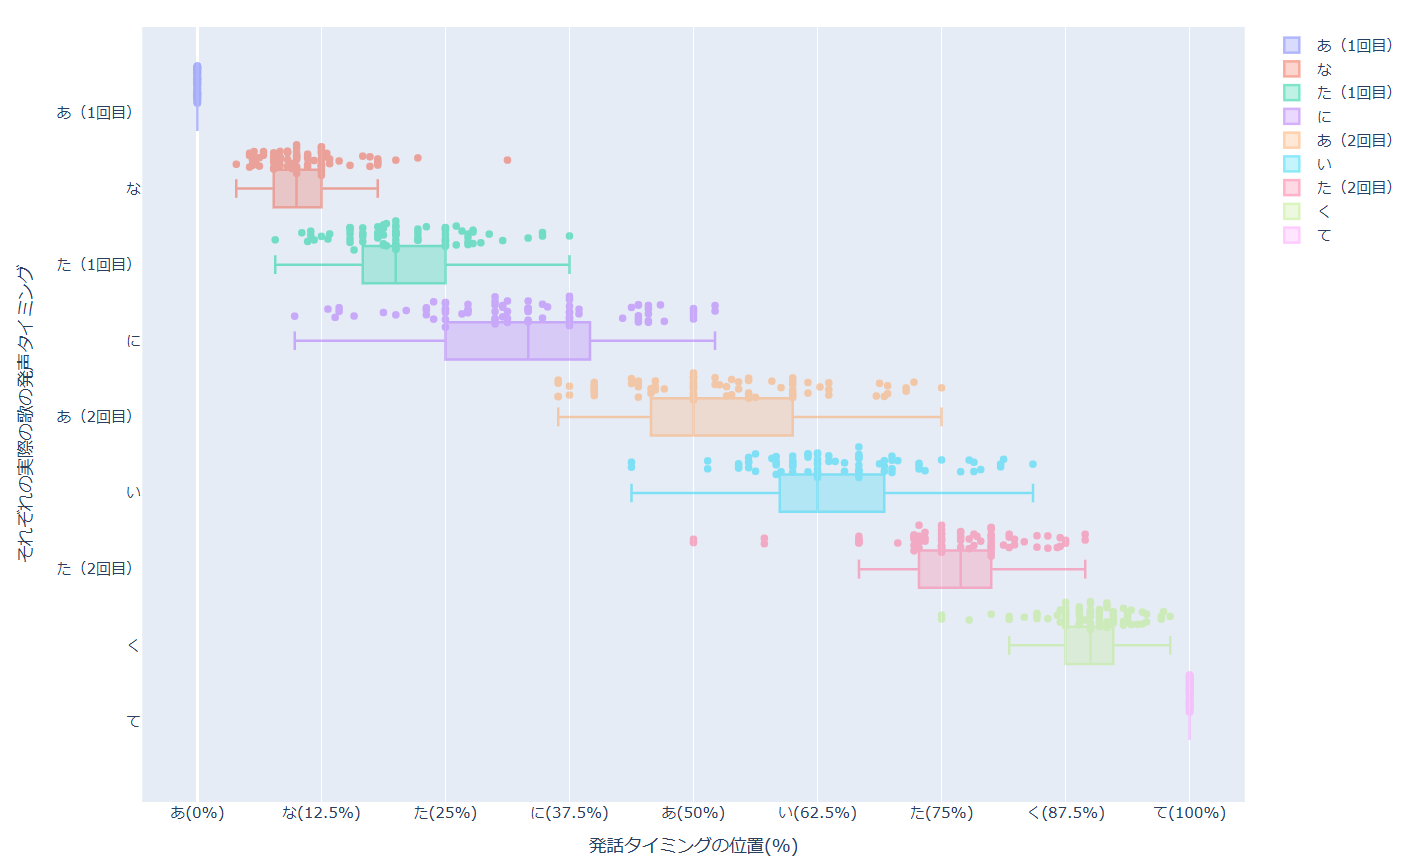
\includegraphics[width=\columnwidth]{fig/anata/2010/tai.png}
    \subcaption{2010年代でのタイミングの違い}
    \label{a_2010_tai}
  \end{minipage}
  \begin{minipage}{0.3\hsize}
    \centering
    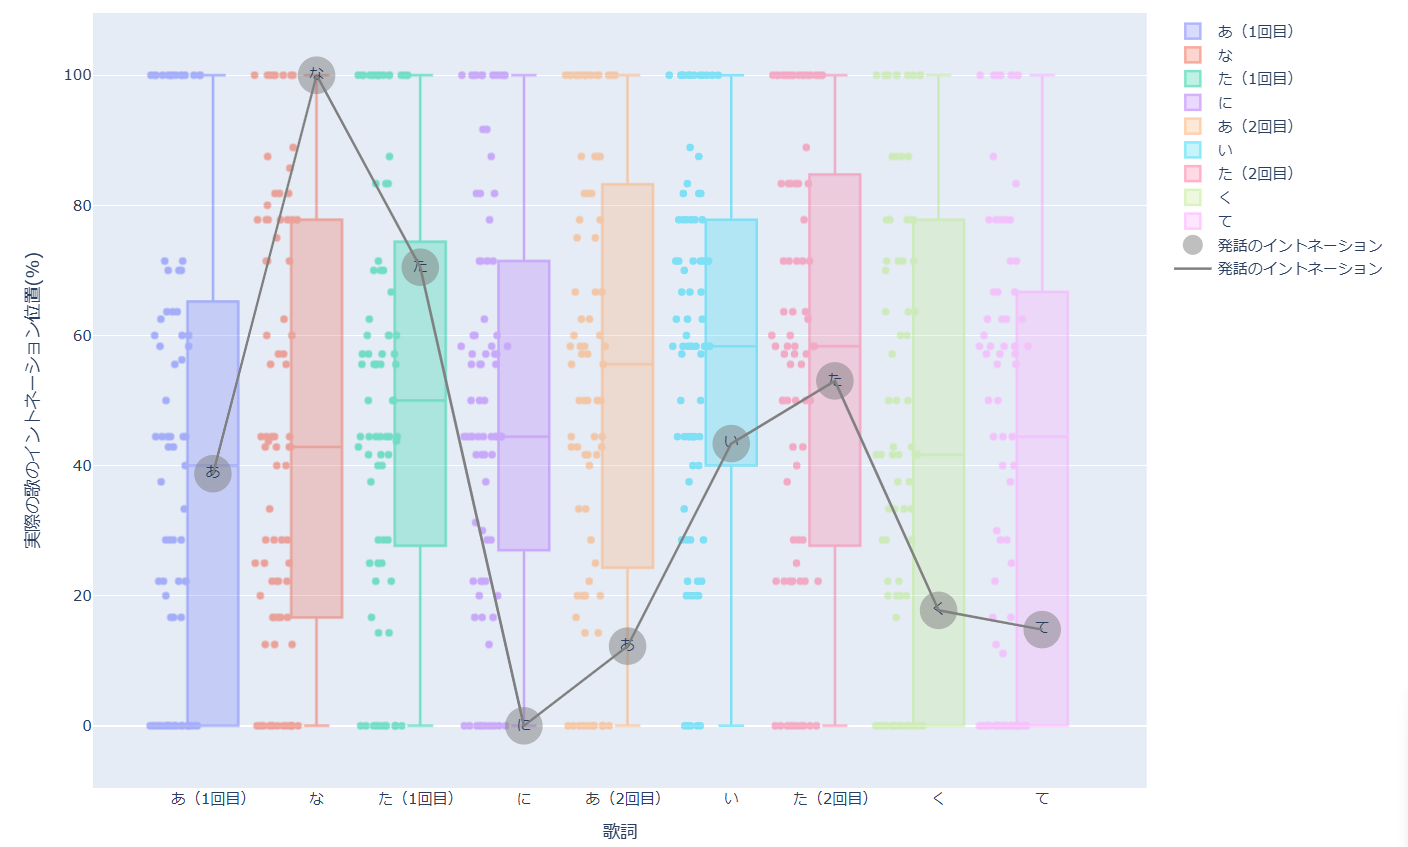
\includegraphics[width=\columnwidth]{fig/anata/2010/int.png}
    \subcaption{2010年代でのイントネーションの違い}
    \label{a_2010_int}
  \end{minipage}
  \begin{minipage}{0.3\hsize}
    \centering
    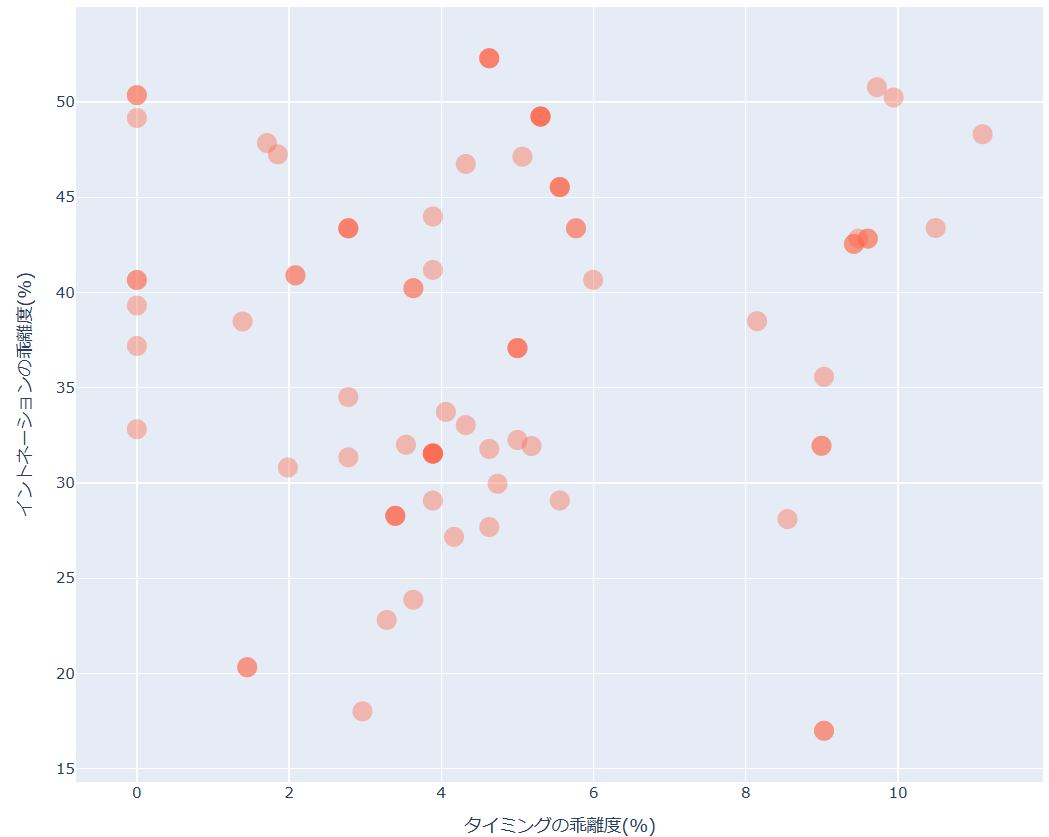
\includegraphics[width=\columnwidth]{fig/anata/2010/tai_int.png}
    \subcaption{2010年代でのタイミングとイントネーションの乖離}
    \label{a_2010_tai_int}
  \end{minipage}
  \caption{「あなたにあいたくて」の2010年代での発話表現との比較}
  \label{a_2010_hakohige}
\end{figure*}

\textbf{“ひかりのほう”での結果}\par
%2010年代のグラフは\figref{h_nendai_2010}である．グラフより，2010年代は「ひかりのほう」は長くとも11拍で歌い切られていることがわかる．また，最高音は76，最低音は47であった．
\figref{h_2010_tai}より，\ref{sec:4.3.1}節と同じく「ひかりのほう」は全て単音において，中央値とタイミングが一致していることがわかる．また，「か」「り」「の」において，第三四分位数が中央値および発話タイミングと一致していることから，75\%の楽曲は発話タイミングと同じか早く発音されており，その中でも25\%から50\%に分布している，つまり25\%の楽曲は発話タイミングと一致して発音されていることがわかる．また「の」において，2つ前の単音の発話タイミングの位置付近まで外れ値があることがわかる．\par
また，\figref{h_2010_int}において，「か」「り」「の」「ほ」「う」において，最大値および第一四分位数が100\%にあることから，各単音の最低でも4分の1がフレーズ内の最も高い音で歌われていることがわかる．\par
また，「ひ」「か」「う」において，第三四分位数が0\%の位置にあることから，各単音の少なくとも4分の1がフレーズ内の最も低い音で歌われていることがわかる．さらに「ひ」については，中央値も0の位置にあることから，少なくとも半分の楽曲がフレーズ内の最も低い音で歌われていることがわかる．\par
さらに，\figref{h_2010_tai_int}において，イントネーションの乖離度は0\%から75\%付近までばらつきがあり，タイミングの乖離度は0\%付近から15\%ほどであるとわかる．また，\ref{sec:4.3.3}と同じく，タイミングの乖離度が0\%の位置，つまり発話タイミングと同じタイミングで歌われている楽曲が固まっていることがわかる．

\begin{figure*}[t]
  \centering
  \begin{minipage}{0.3\hsize}
    \centering
    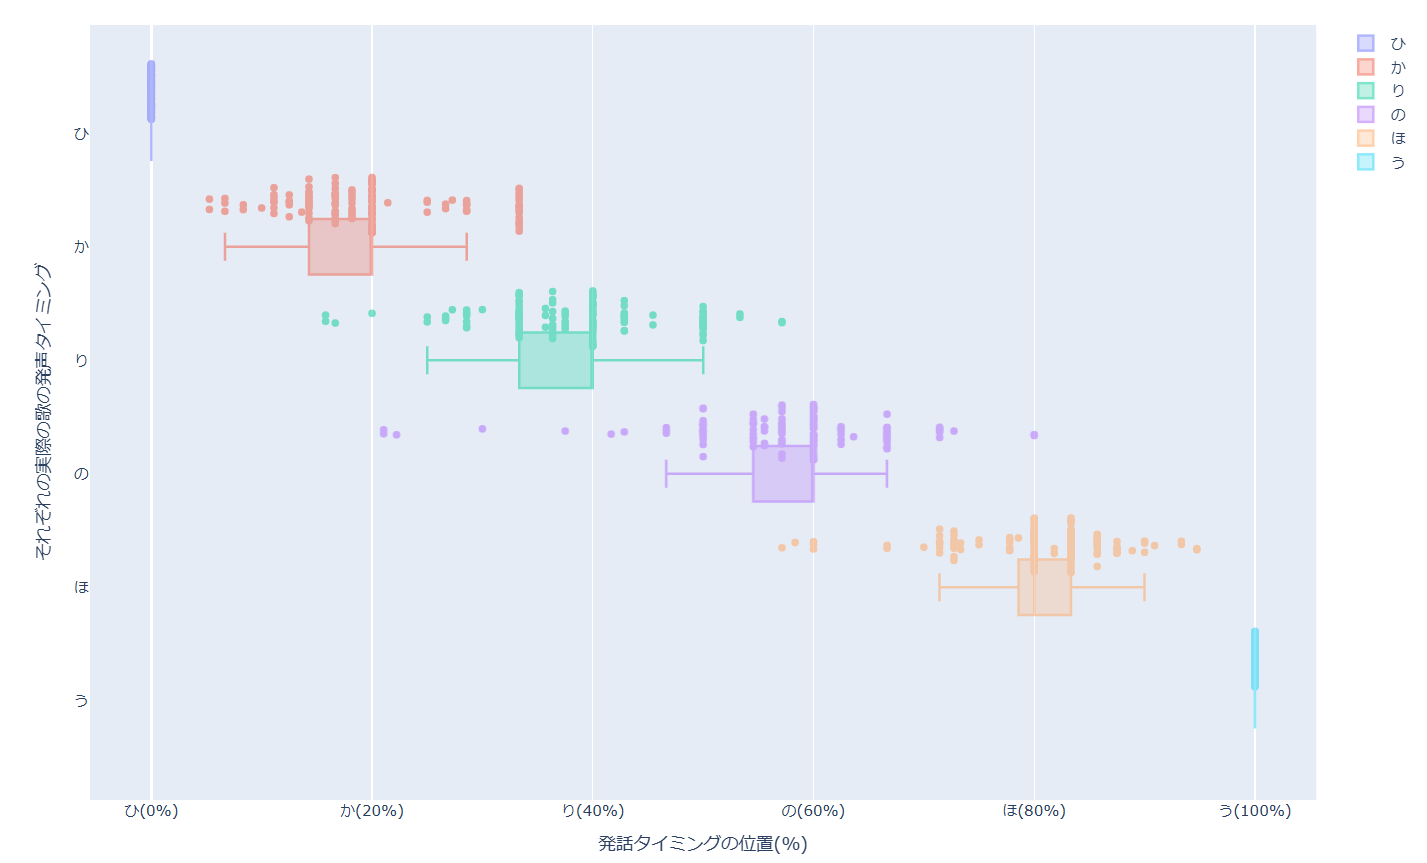
\includegraphics[width=\columnwidth]{fig/hikari/2010/tai.png}
    \subcaption{2010年代でのタイミングの違い}
    \label{h_2010_tai}
  \end{minipage}
  \begin{minipage}{0.3\hsize}
    \centering
    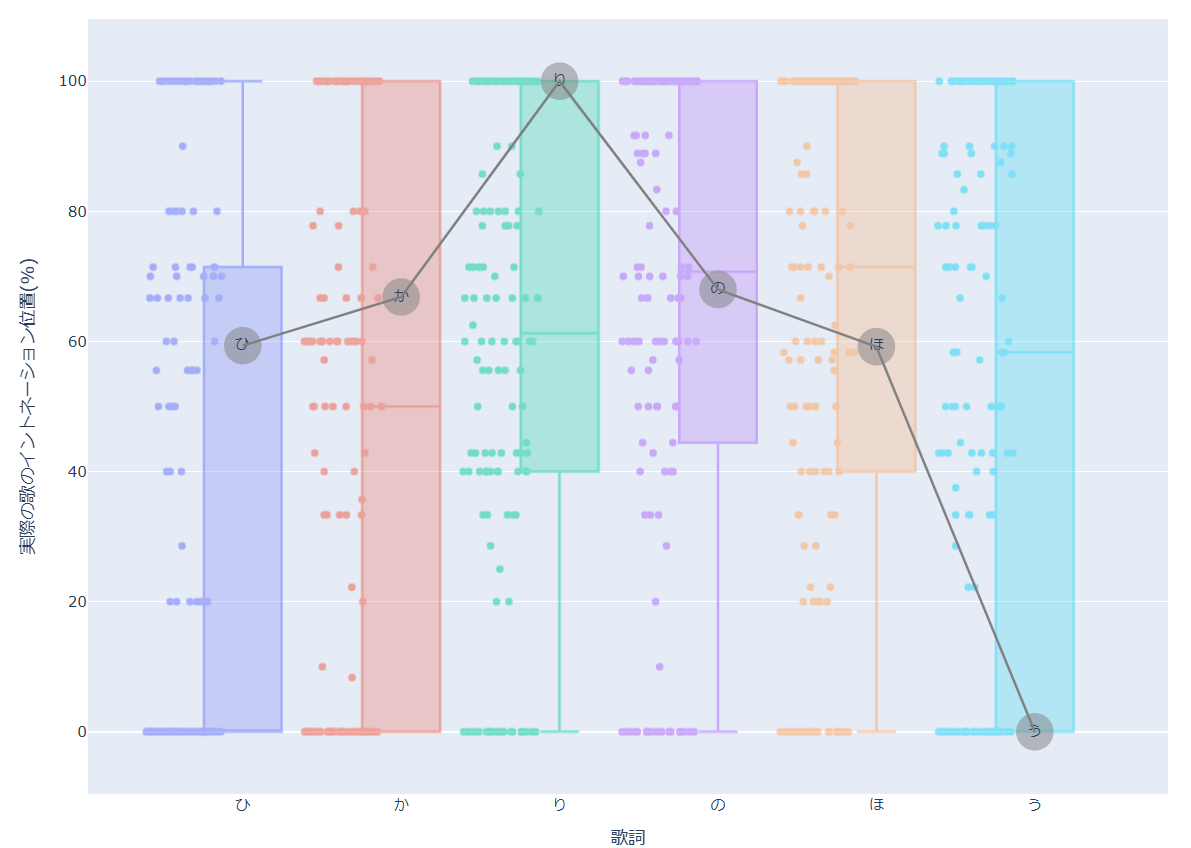
\includegraphics[width=\columnwidth]{fig/hikari/2010/int.png}
    \subcaption{2010年代でのイントネーションの違い}
    \label{h_2010_int}
  \end{minipage}
  \begin{minipage}{0.3\hsize}
    \centering
    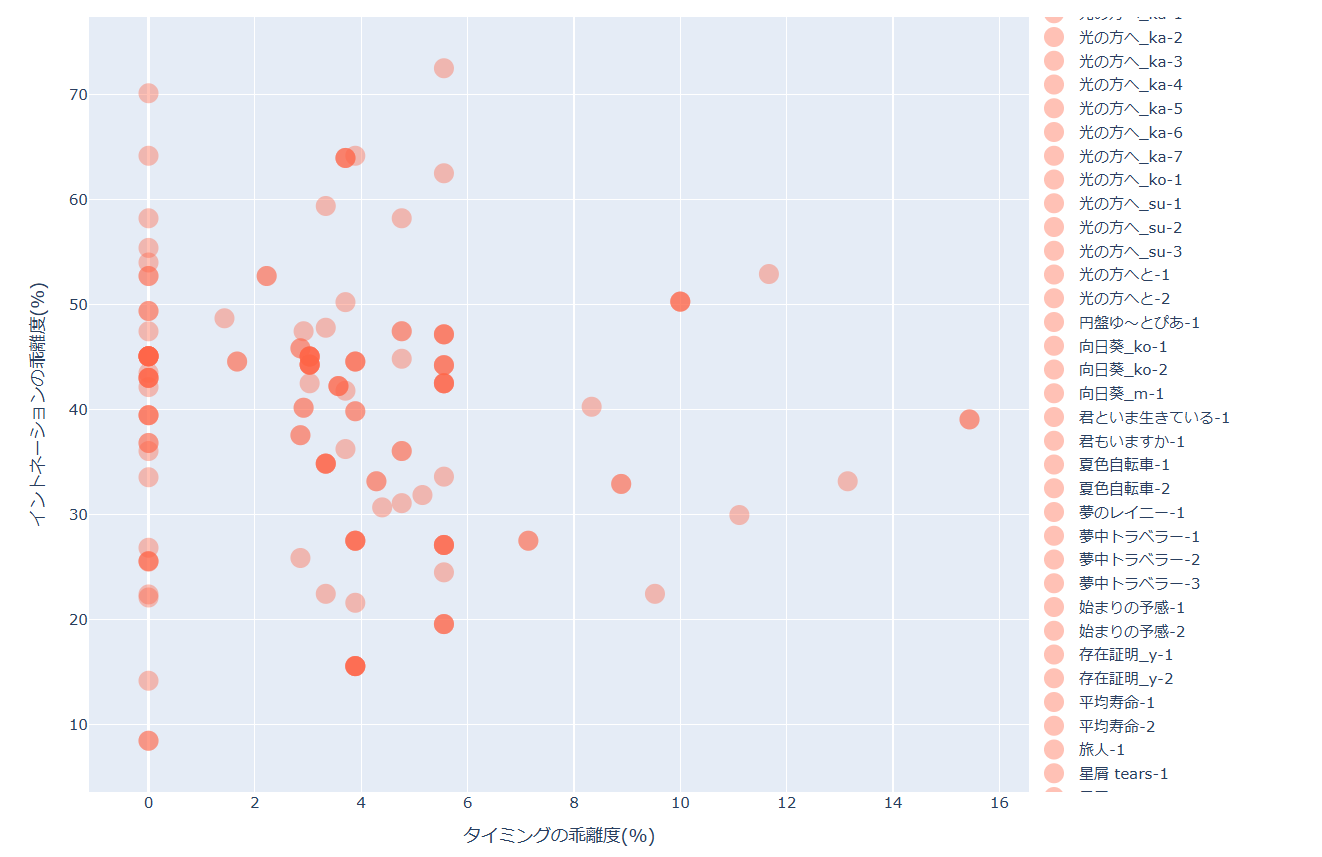
\includegraphics[width=\columnwidth]{fig/hikari/2010/tai_int.png}
    \subcaption{2010年代でのタイミングとイントネーションの乖離}
    \label{h_2010_tai_int}
  \end{minipage}
  \caption{「ひかりのほう」の2010年代での発話表現との比較}
  \label{h_2010_hakohige}
\end{figure*}

%4.4.6
\subsubsection{2020年代のグラフ}

\textbf{“あなたにあいたくて”での結果}\par
%2020年代のグラフはこれ\ref{a_nendai_2020}．グラフより，2020年代は「あなたにあいたくて」は長くとも24拍で歌い切られていることがわかる．また，最高音は75，最低音は50であった．\par
\figref{a_2020_tai}より，「あ（1回目）」において，中央値が発話タイミングと一致していることがわかる．また，「に」「た（1回目）」において，ひげがかなり長いことから，歌唱タイミングが幅広いことを示している．\par
また，\figref{a_2020_int}より，「あ（1回目）」「に」「く」「て」において，第三四分位数が0\%の位置にあることから，少なくとも4分の1が最も低い音で歌われていることがわかる．また，「い」について，最大値および第一四分位数が100\%にあることから，各単音の最低でも4分の1がフレーズ内の最も高い音で歌われていることがわかる．\par
さらに，\figref{a_2020_tai_int}において，イントネーションの乖離度は23\%から55\%となっており，タイミングの乖離度は0\%から13\%ほどであるとわかる．
\begin{figure*}[t]
  \centering
  \begin{minipage}{0.3\hsize}
    \centering
    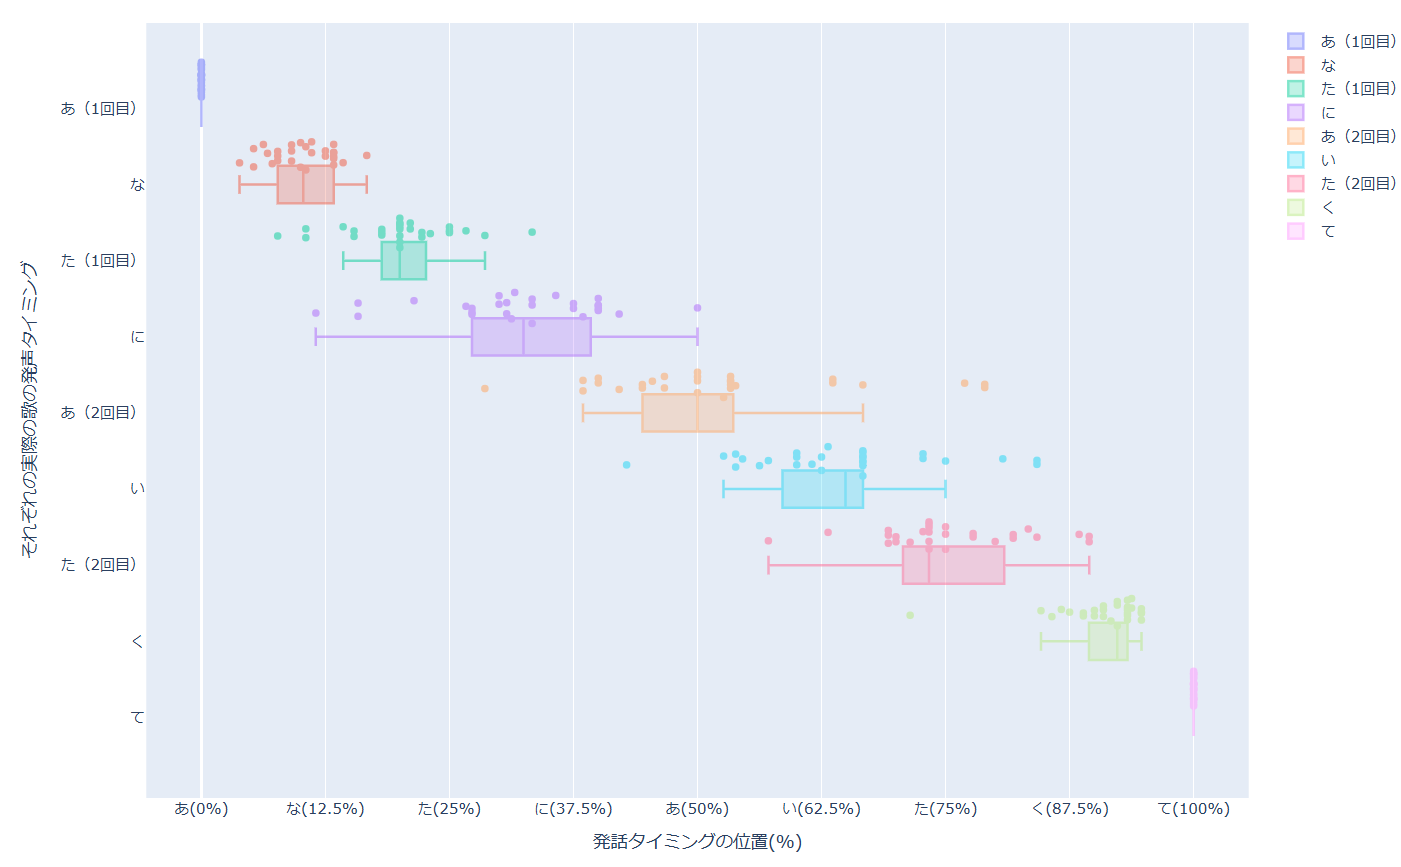
\includegraphics[width=\columnwidth]{fig/anata/2020/tai.png}
    \subcaption{2020年代でのタイミングの違い}
    \label{a_2020_tai}
  \end{minipage}
  \begin{minipage}{0.3\hsize}
    \centering
    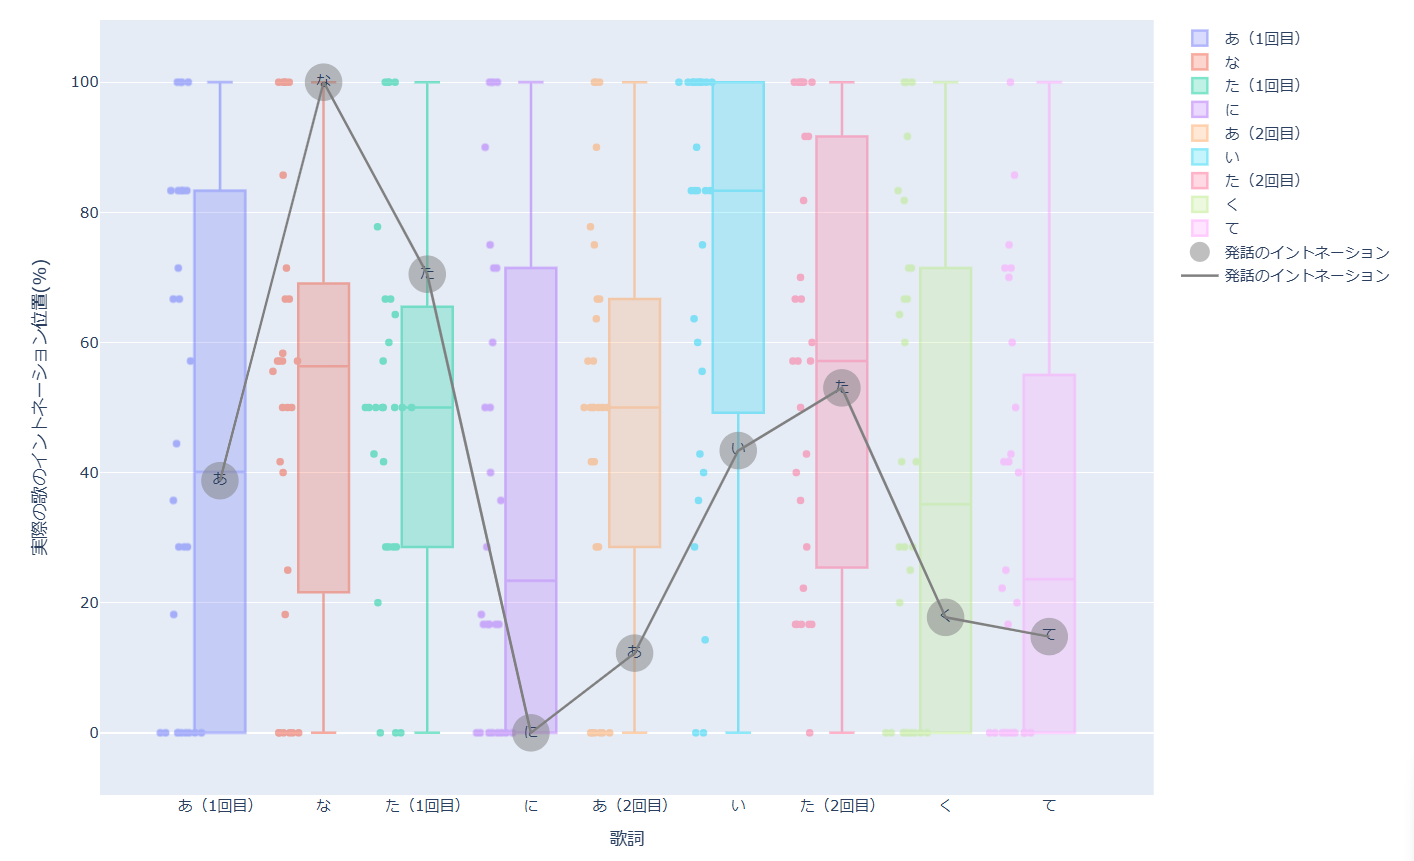
\includegraphics[width=\columnwidth]{fig/anata/2020/int.png}
    \subcaption{2020年代でのイントネーションの違い}
    \label{a_2020_int}
  \end{minipage}
  \begin{minipage}{0.3\hsize}
    \centering
    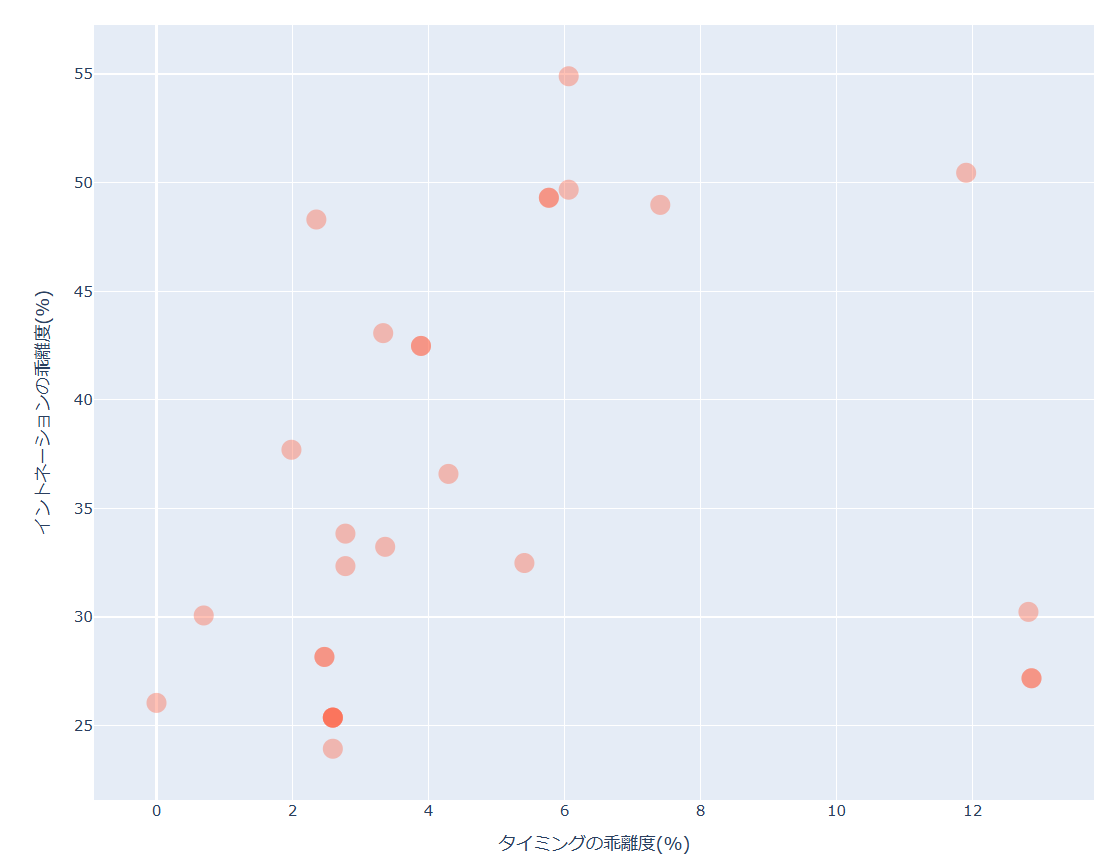
\includegraphics[width=\columnwidth]{fig/anata/2020/tai_int.png}
    \subcaption{2020年代でのタイミングとイントネーションの乖離}
    \label{a_2020_tai_int}
  \end{minipage}
  \caption{「あなたにあいたくて」の2020年代での発話表現との比較}
  \label{a_2020_hakohige}
\end{figure*}

\textbf{“ひかりのほう”での結果}\par
%2020年代のグラフは\figref{h_nendai_2020}である．グラフより，2020年代は「ひかりのほう」は長くとも12拍で歌い切られていることがわかる．また，最高音は76，最低音は45であった．
\figref{h_2020_tai}より，「か」「り」のみ中央値とタイミングの不一致が起こっている．また，「か」において，第三四分位数と発話タイミングが一致していることから，75\%のフレーズが発話タイミングと同じか早く発音されている．また，「ほ」において，2つ前の単音の発話タイミングの位置付近まで外れ値があることがわかる．\par
また，\figref{h_2020_int}において，「か」「り」「の」「ほ」において，最大値および第一四分位数が100\%にあることから，各単音の最低でも4分の1がフレーズ内の最も高い音で歌われていることがわかる．\par
また，「ひ」「う」において，第三四分位数が0\%の位置にあることから，各単音の少なくとも4分の1がフレーズ内の最も低い音で歌われていることがわかる．さらに「ひ」については，中央値も0の位置にあることから，少なくとも半分の楽曲がフレーズ内の最も低い音で歌われていることがわかる．\par
さらに，\figref{h_2020_tai_int}において，イントネーションの乖離度は0\%から63\%付近までばらつきがあり，タイミングの乖離度は0\%付近から15\%ほどであるとわかる．
\begin{figure*}[t]
  \centering
  \begin{minipage}{0.3\hsize}
    \centering
    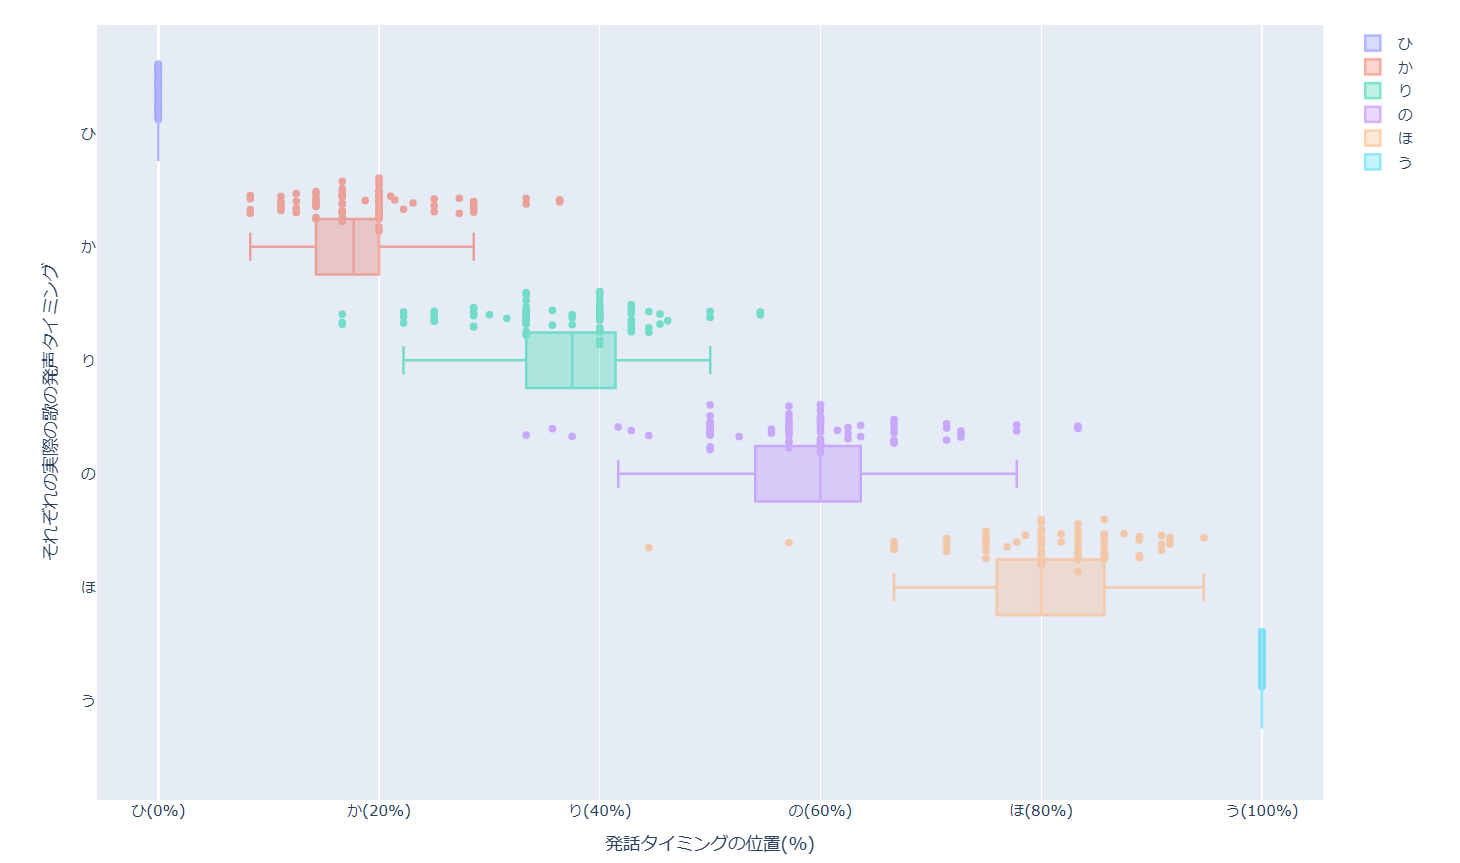
\includegraphics[width=\columnwidth]{fig/hikari/2020/tai.png}
    \subcaption{2020年代でのタイミングの違い}
    \label{h_2020_tai}
  \end{minipage}
  \begin{minipage}{0.3\hsize}
    \centering
    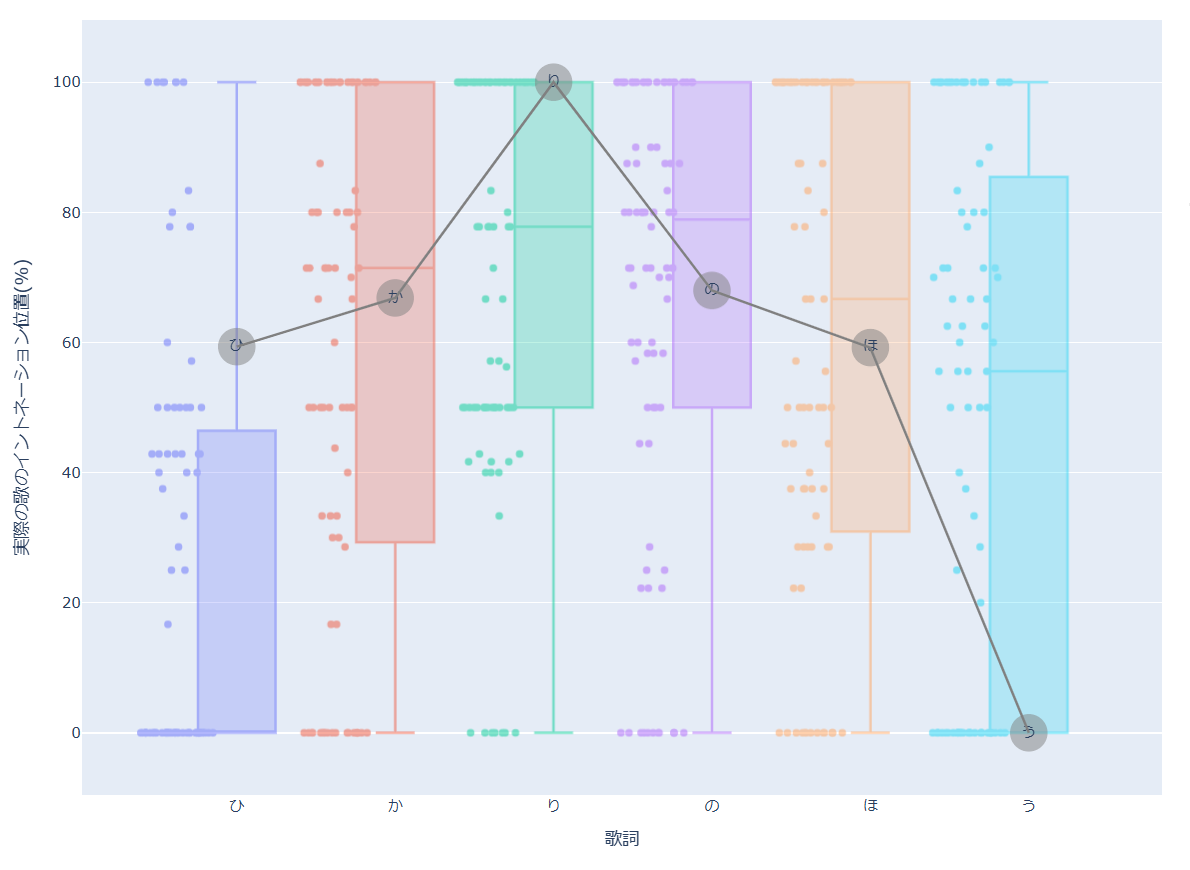
\includegraphics[width=\columnwidth]{fig/hikari/2020/int.png}
    \subcaption{2020年代でのイントネーションの違い}
    \label{h_2020_int}
  \end{minipage}
  \begin{minipage}{0.3\hsize}
    \centering
    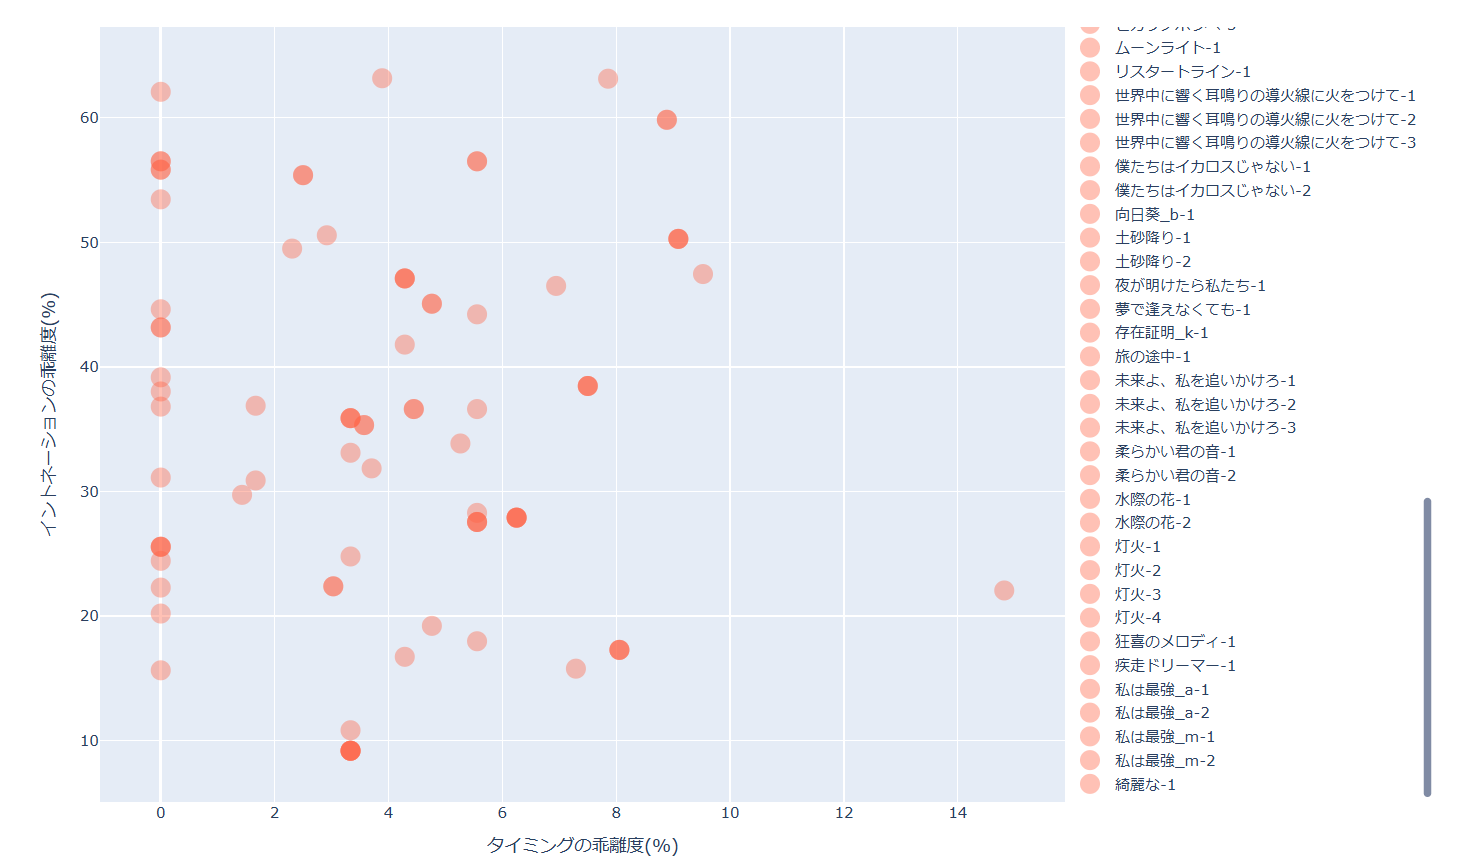
\includegraphics[width=\columnwidth]{fig/hikari/2020/tai_int.png}
    \subcaption{2020年代でのタイミングとイントネーションの乖離}
    \label{h_2020_tai_int}
  \end{minipage}
  \caption{「ひかりのほう」の2020年代での発話表現との比較}
  \label{h_2020_hakohige}
\end{figure*}


%4.5
\subsection{表拍・裏拍の割合}\label{sec:4.5}
次に，表拍・裏拍の割合をグラフに起こしていく．\par
表拍・裏拍とは，一つの拍を2分割したときの区別の方法で，前の方を表拍，後ろの方を裏拍という\cite{omotehaku_urahaku}．今回の研究で使われている，4分の4拍子，4分の3拍子，8分の6拍子の表拍・裏拍を表に起こすと，\tabref{omoura_44}，\tabref{omoura_34}，\tabref{omoura_68}になる．

\begin{table}[htb]
  \centering
  \caption{4分の4拍子での表拍・裏拍}
  \begin{tabular}{|c||c|c|c|c|c|c|c|c|} \hline
    拍     & \multicolumn{2}{|c|}{1} & \multicolumn{2}{|c|}{2} & \multicolumn{2}{|c|}{3} & \multicolumn{2}{|c|}{4}                     \\ \hline\hline
    オフセット & 0                       & 0.5                     & 1                       & 1.5                     & 2 & 2.5 & 3 & 3.5 \\ \hline
    表裏    & 表                       & 裏                       & 表                       & 裏                       & 表 & 裏   & 表 & 裏   \\ \hline
  \end{tabular}
  \label{omoura_44}
\end{table}

\begin{table}[htb]
  \centering
  \caption{4分の3拍子での表拍・裏拍}
  \begin{tabular}{|c||c|c|c|c|c|c|} \hline
    拍     & \multicolumn{2}{|c|}{1} & \multicolumn{2}{|c|}{2} & \multicolumn{2}{|c|}{3}                 \\ \hline\hline
    オフセット & 0                       & 0.5                     & 1                       & 1.5 & 2 & 2.5 \\ \hline
    表裏    & 表                       & 裏                       & 表                       & 裏   & 表 & 裏   \\ \hline
  \end{tabular}
  \label{omoura_34}
\end{table}

\begin{table}[htb]
  \centering
  \caption{8分の6拍子での表拍・裏拍}
  \begin{tabular}{|c||c|c|c|c|c|c|} \hline
    拍     & \multicolumn{3}{|c|}{1} & \multicolumn{3}{|c|}{2}                     \\ \hline\hline
    オフセット & 0                       & 0.5                     & 1 & 1.5 & 2 & 2.5 \\ \hline
    表裏    & 表                       & 裏                       & 裏 & 表   & 裏 & 裏   \\ \hline
  \end{tabular}
  \label{omoura_68}
\end{table}

\textbf{“あなたにあいたくて”での結果}\par
各拍子での表拍・裏拍を棒グラフで可視化したのが，\figref{a_44}，\figref{a_34}，\figref{a_68}である．


\begin{figure*}[t]
  \centering
  \begin{minipage}{0.3\hsize}
    \centering
    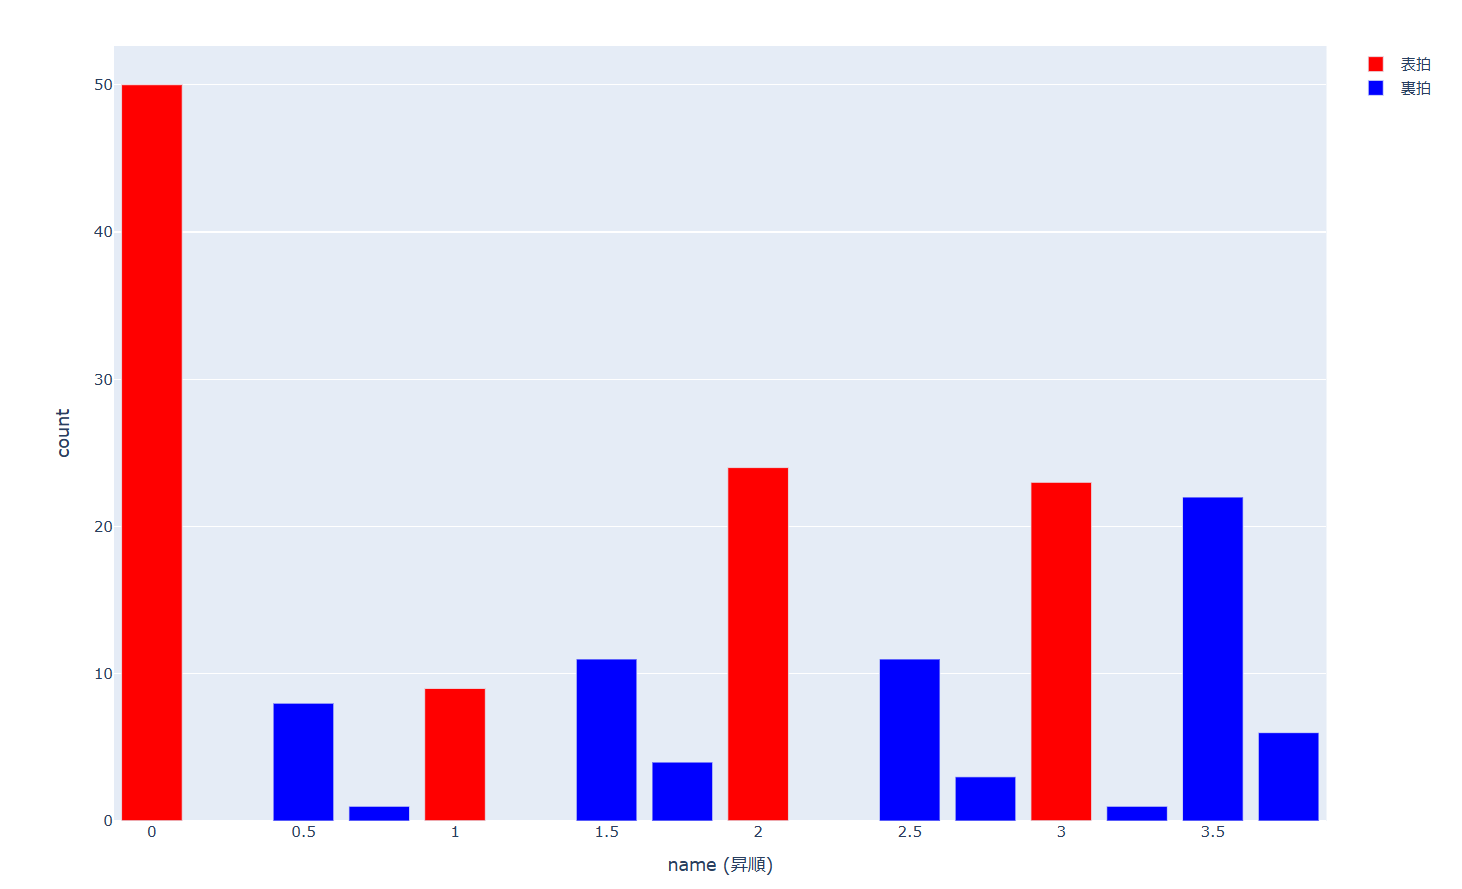
\includegraphics[width=\columnwidth]{fig/anata/a_44.png}
    \subcaption{4分の4拍子の表拍・裏拍の分布}
    \label{a_44}
  \end{minipage}
  \begin{minipage}{0.3\hsize}
    \centering
    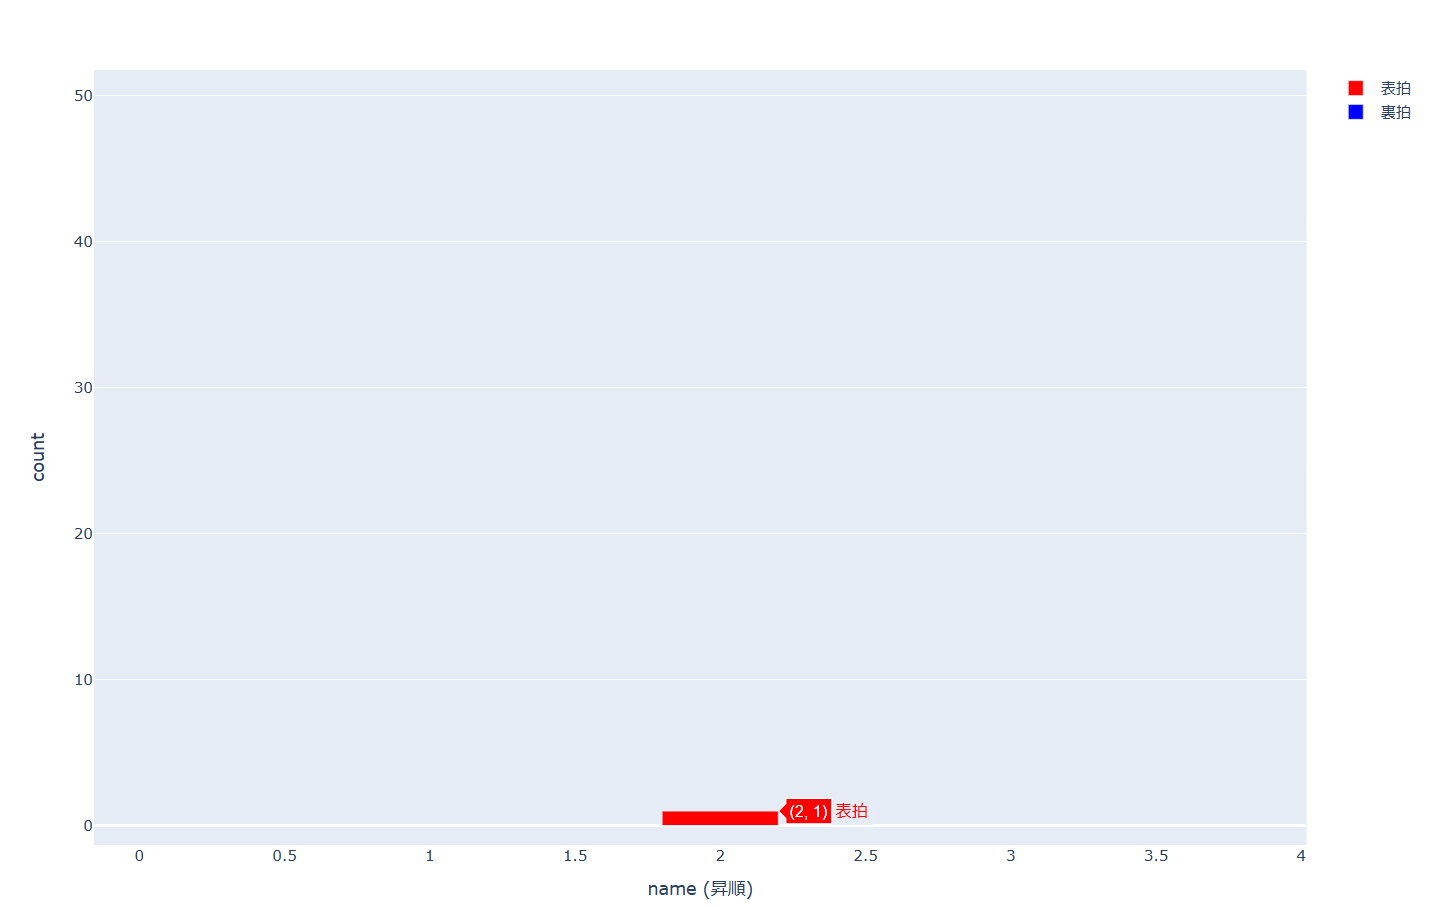
\includegraphics[width=\columnwidth]{fig/anata/a_34.png}
    \subcaption{4分の3拍子の表拍・裏拍の分布}
    \label{a_34}
  \end{minipage}
  \begin{minipage}{0.3\hsize}
    \centering
    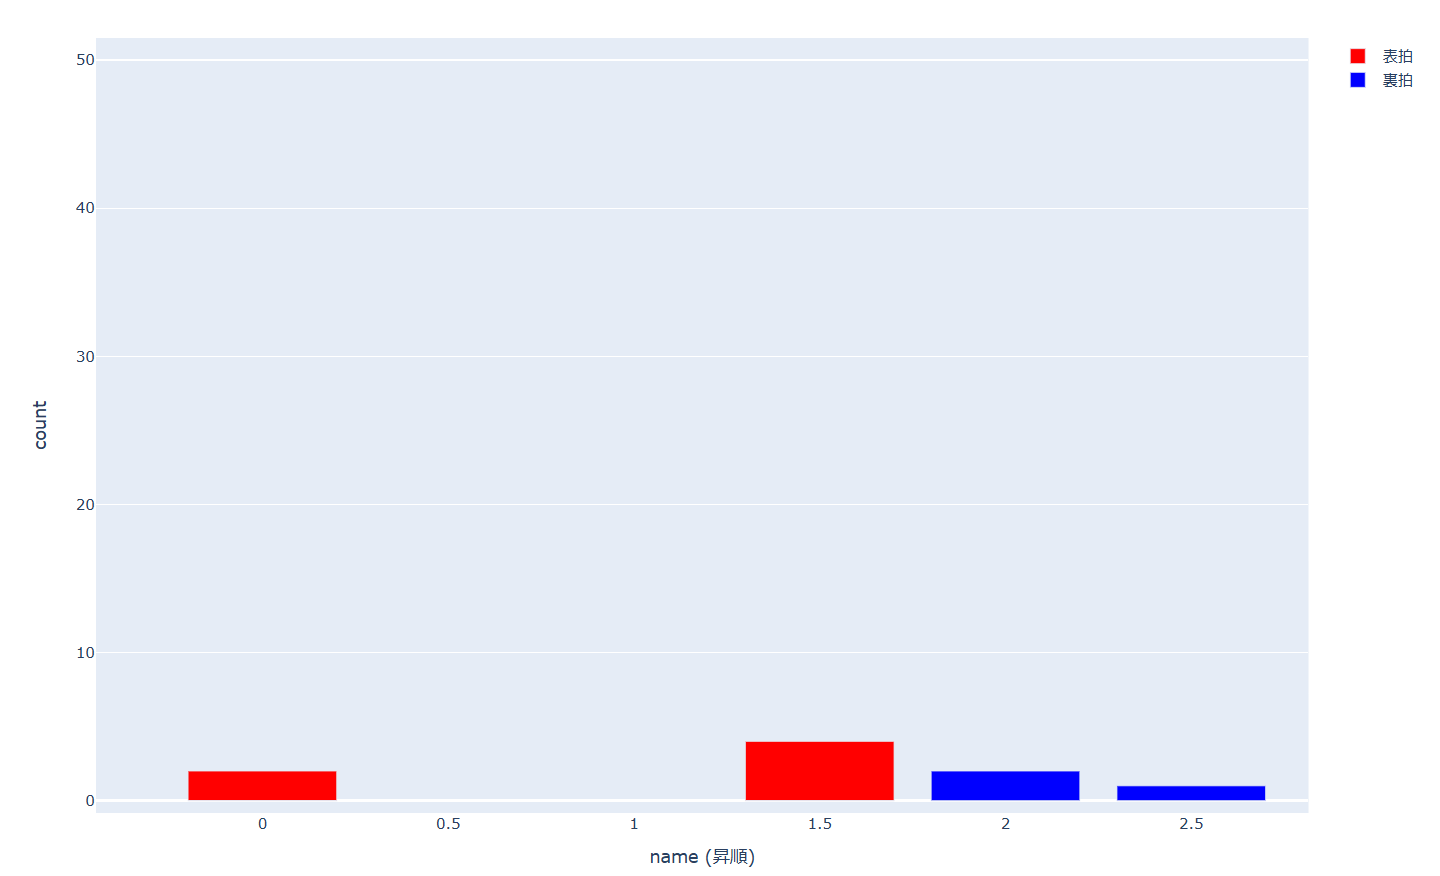
\includegraphics[width=\columnwidth]{fig/anata/a_68.png}
    \subcaption{8分の6拍子の表拍・裏拍の分布}
    \label{a_68}
  \end{minipage}
  \caption{「あなたにあいたくて」の表拍・裏拍の分布}
  \label{a_omoura}
\end{figure*}


\figref{a_44}，\figref{a_34}，\figref{a_68}より，最も多いタイミングは4分の4拍子の1拍目表拍での歌唱であることがわかる．また，3拍目表拍や4拍目表拍も多く，「あなたにあいたくて」は表拍で歌われている楽曲が多いとわかる．\par
また，裏拍で歌われている拍で最も多いのは4分の4拍子の4.5拍目であることがわかる．

\textbf{“ひかりのほう”での結果}\par
各拍子での表拍・裏拍を棒グラフで可視化したのが，\figref{h_44}，\figref{h_34}，\figref{h_68}である．

\begin{figure*}[t]
  \centering
  \begin{minipage}{0.3\hsize}
    \centering
    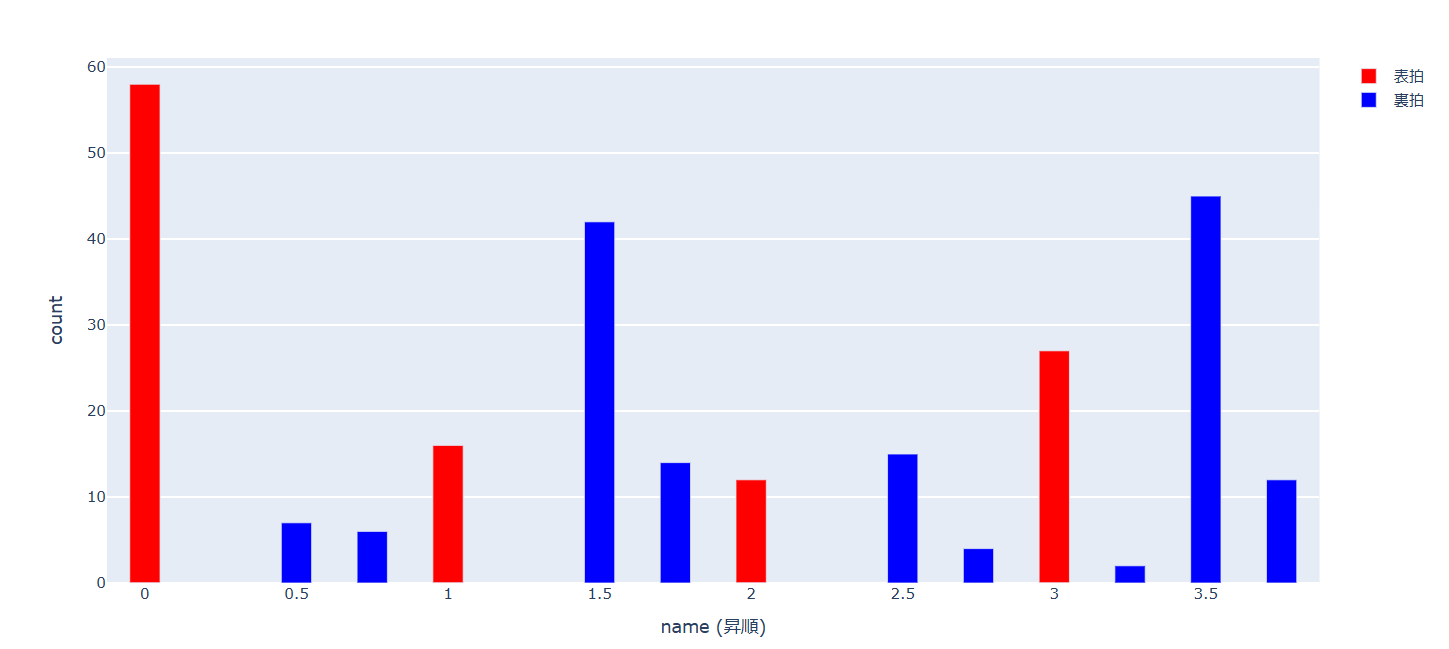
\includegraphics[width=\columnwidth]{fig/hikari/hi_44.png}
    \subcaption{4分の4拍子の表拍・裏拍の分布}
    \label{h_44}
  \end{minipage}
  \begin{minipage}{0.3\hsize}
    \centering
    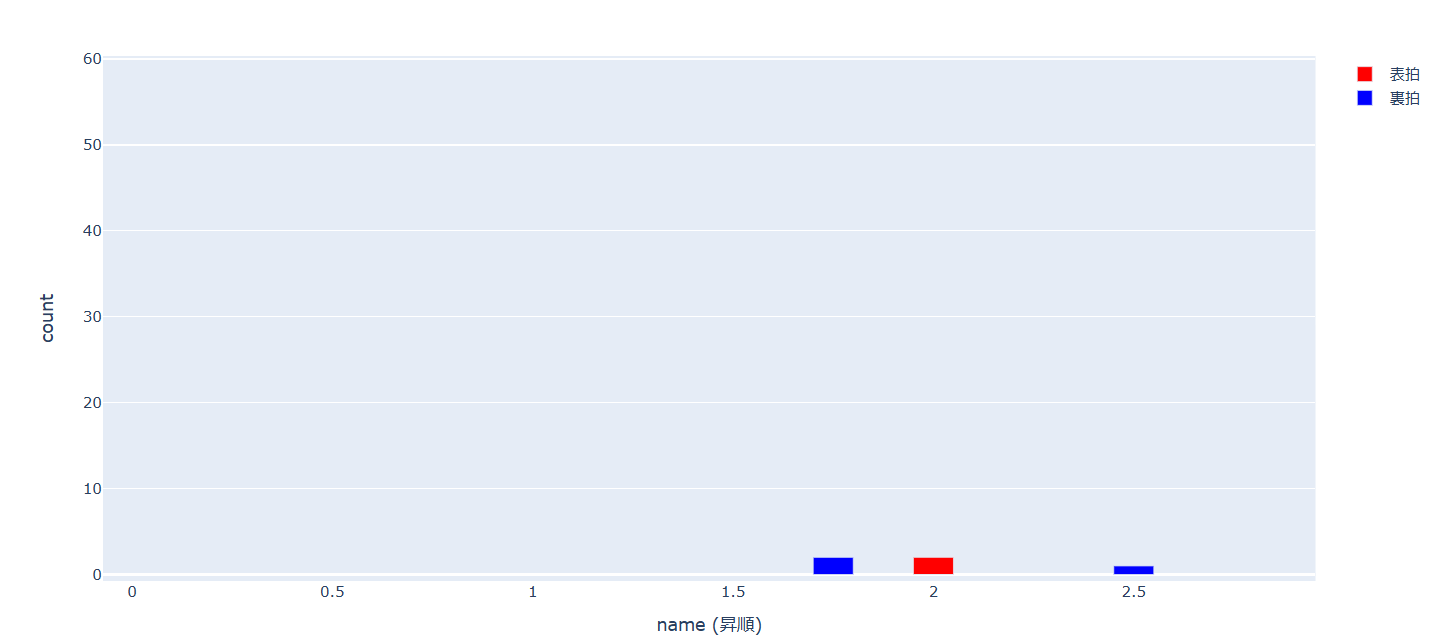
\includegraphics[width=\columnwidth]{fig/hikari/hi_34.png}
    \subcaption{4分の3拍子の表拍・裏拍の分布}
    \label{h_34}
  \end{minipage}
  \begin{minipage}{0.3\hsize}
    \centering
    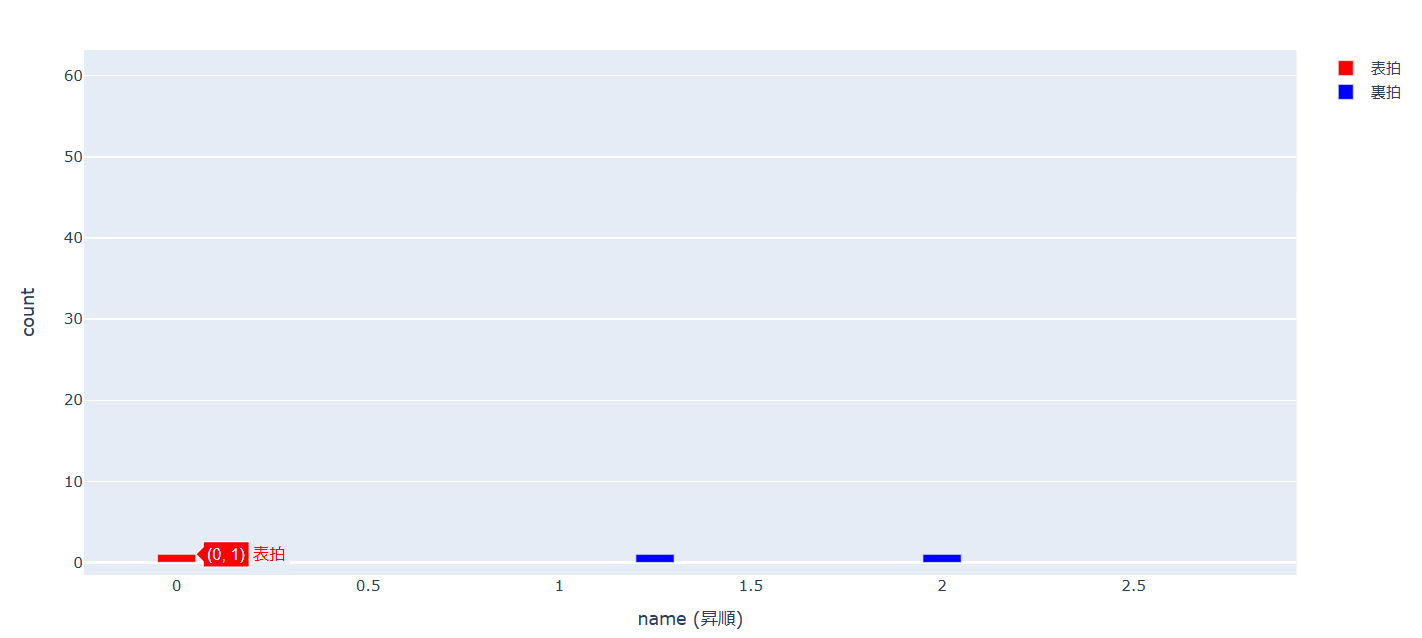
\includegraphics[width=\columnwidth]{fig/hikari/hi_68.png}
    \subcaption{8分の6拍子の表拍・裏拍の分布}
    \label{h_68}
  \end{minipage}
  \caption{「あなたにあいたくて」の表拍・裏拍の分布}
  \label{h_omoura}
\end{figure*}

\figref{h_44}，\figref{h_34}，\figref{h_68}より，最も多いタイミングは4分の4拍子の1拍目表拍での歌唱であることがわかる．また4分の4拍子2拍目裏拍，4拍目裏拍も多いことがわかる．\par
また，出現回数を合計すると裏拍の数が多いため，「ひかりのほう」では裏拍で歌われることが多いことがわかる．

\subsection{音高の分布図}
各フレーズの各単音において，どの高さの音が多いのか，どのように分布をしているのかを以下のグラフに示す．\par
\subsubsection{全体の結果}
\begin{figure*}[t]
  \centering
  \begin{minipage}{0.49\hsize}
    \centering
    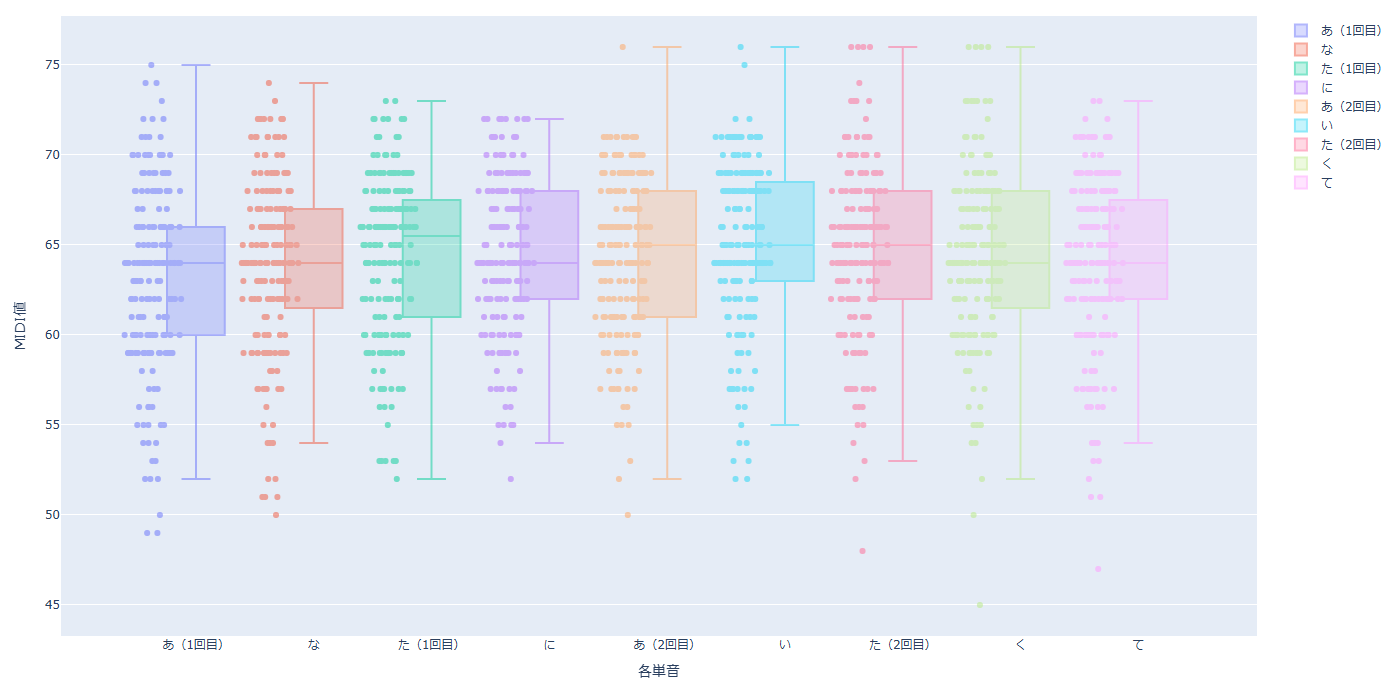
\includegraphics[width=\columnwidth]{fig/anata/midi/zentai.png}
    \subcaption{“あなたにあいたくて”}
    \label{a_midi_zentai}
  \end{minipage}
  \begin{minipage}{0.49\hsize}
    \centering
    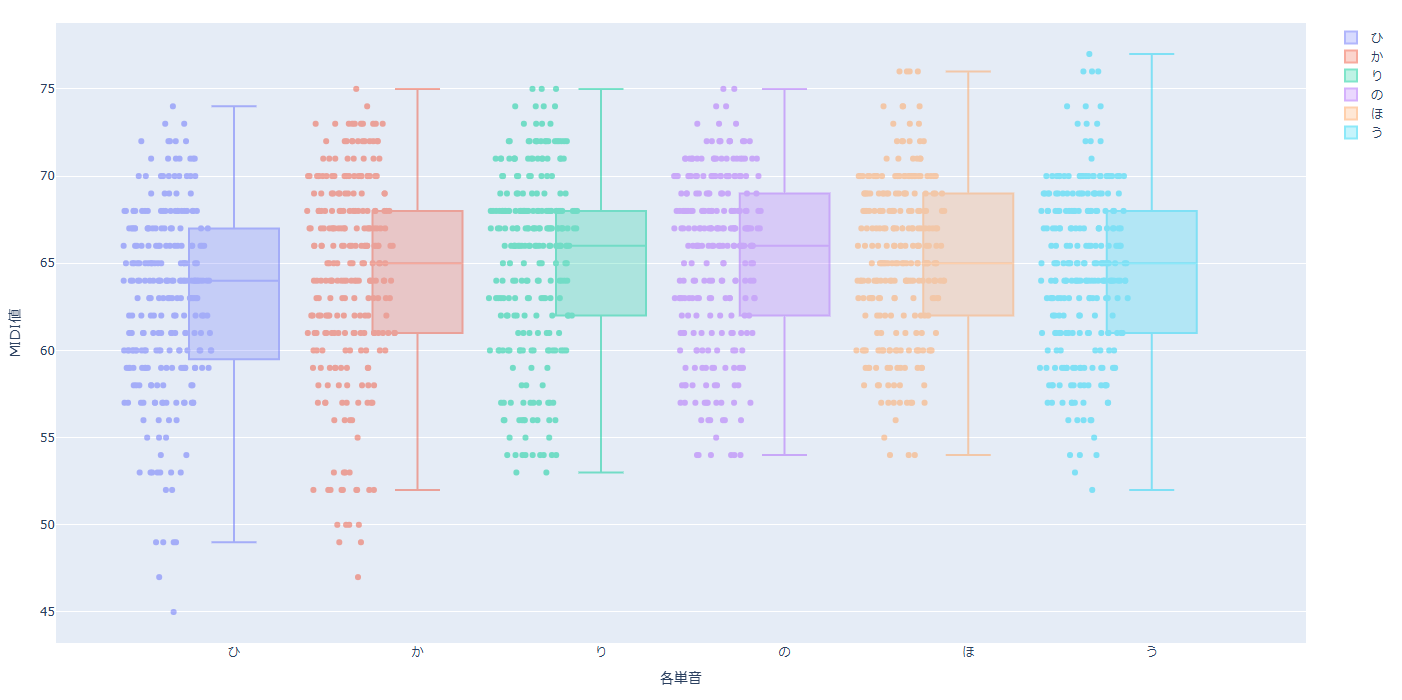
\includegraphics[width=\columnwidth]{fig/hikari/midi/zentai.png}
    \subcaption{“ひかりのほう”}
    \label{h_midi_zentai}
  \end{minipage}
  \caption{音高（MIDIナンバー）の全体の分布}
  \label{midi_zentai}
\end{figure*}

\textbf{“あなたにあいたくて”での結果}\par
\figref{a_midi_zentai}により，それぞれ第三四分位数は68付近，中央値は65付近，第一四分位数は61付近となっており，それぞれ比較しての違いはあまり見られないことがわかる．また，「あなたに」と進むにつれてひげがちいさくなっていき，「あ（2回目）」でまたひげが大きくなると，「て」で狭まっていることがわかる．

\textbf{“ひかりのほう”での結果}\par
\figref{h_midi_zentai}により，それぞれ第三四分位数は68付近，中央値は65付近，第一四分位数は61付近となっており，それぞれ比較しての違いはあまり見られないことがわかる．また，最高値に関しては，「ひかりのほう」と進んでいくにつれて高くなっていっている．また，最低値に関して，「ひかり」で徐々に上がり，「う」で下がっていくことがわかる．

\subsubsection{男性のみでの結果}
\begin{figure*}[t]
  \centering
  \begin{minipage}{0.49\hsize}
    \centering
    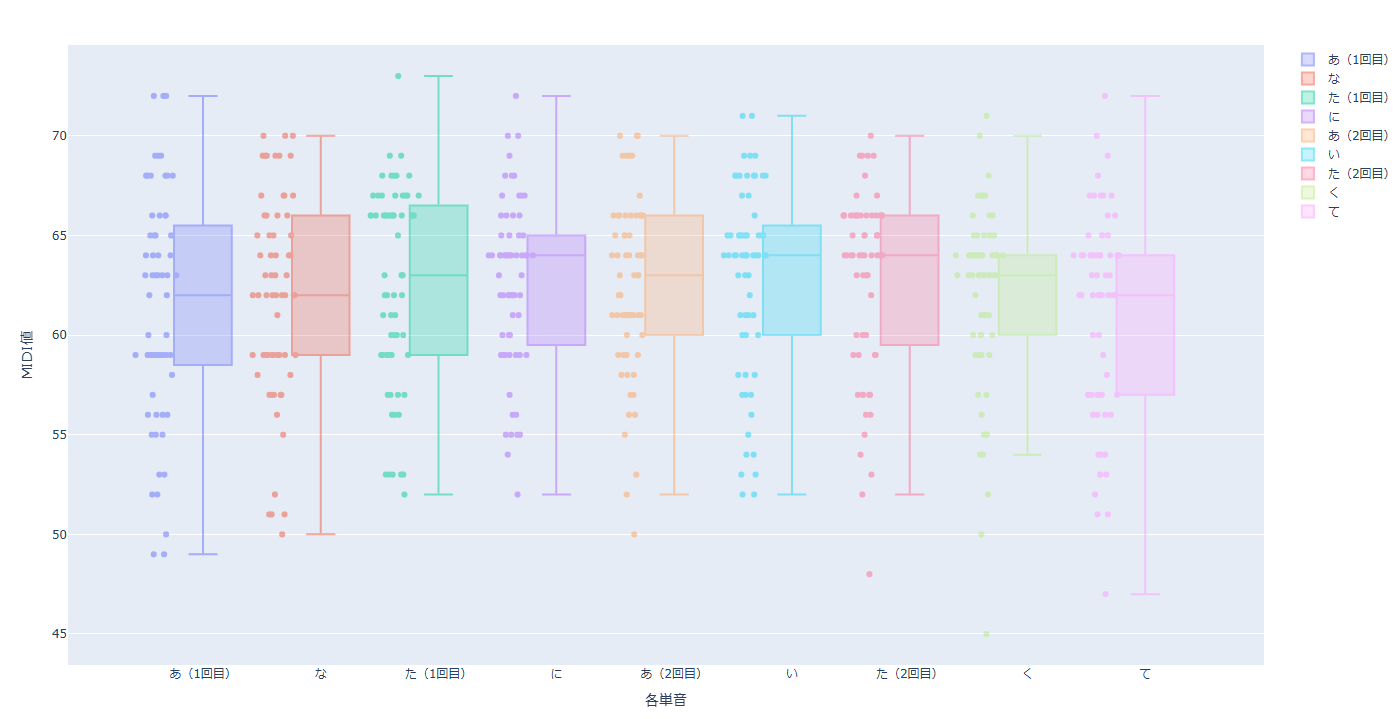
\includegraphics[width=\columnwidth]{fig/anata/midi/otoko.png}
    \subcaption{“あなたにあいたくて”}
    \label{a_midi_otoko}
  \end{minipage}
  \begin{minipage}{0.49\hsize}
    \centering
    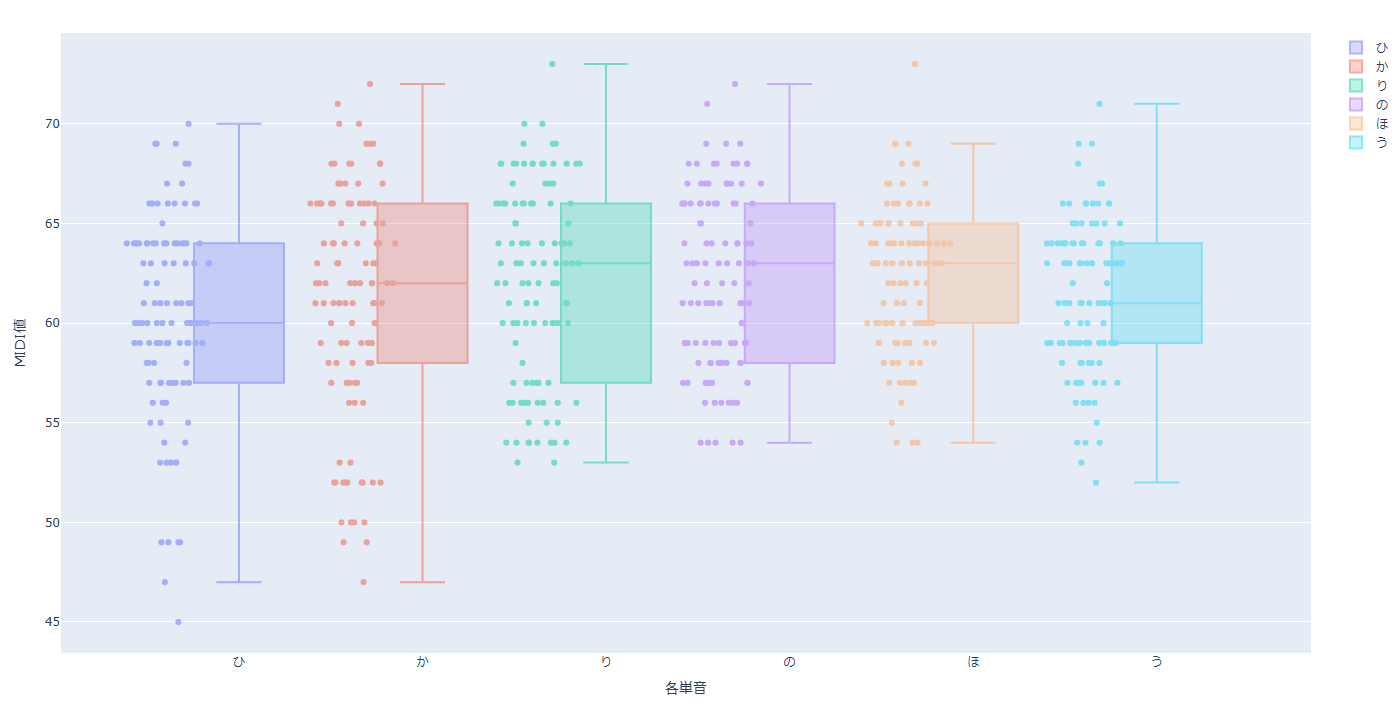
\includegraphics[width=\columnwidth]{fig/hikari/midi/otoko.png}
    \subcaption{“ひかりのほう”}
    \label{h_midi_otoko}
  \end{minipage}
  \caption{音高（MIDIナンバー）の男性の分布}
  \label{midi_otoko}
\end{figure*}

\textbf{“あなたにあいたくて”での結果}\par
\figref{a_midi_otoko}により，「く」において，箱が他の単音と比べて狭いことから，ばらつきが少ないことがわかる．また，「て」において，ひげがかなり長いことから，\figref{a_midi_zentai}と比較して，かなり広い音域をカバーしているのがわかる．

\textbf{“ひかりのほう”での結果}\par
\figref{h_midi_otoko}により，「ほ」において，箱やひげが他の単音と比べて狭いことから，かなりばらつきが少ないことがわかる．また，「ひ」「か」に関して低めの音が集まっているのがわかる．\par
また，「ひ」「か」において，\figref{h_midi_zentai}と比較して,かなり広い音域をカバーしているのがわかる．


\subsubsection{女性のみでの結果}
\begin{figure*}[t]
  \centering
  \begin{minipage}{0.49\hsize}
    \centering
    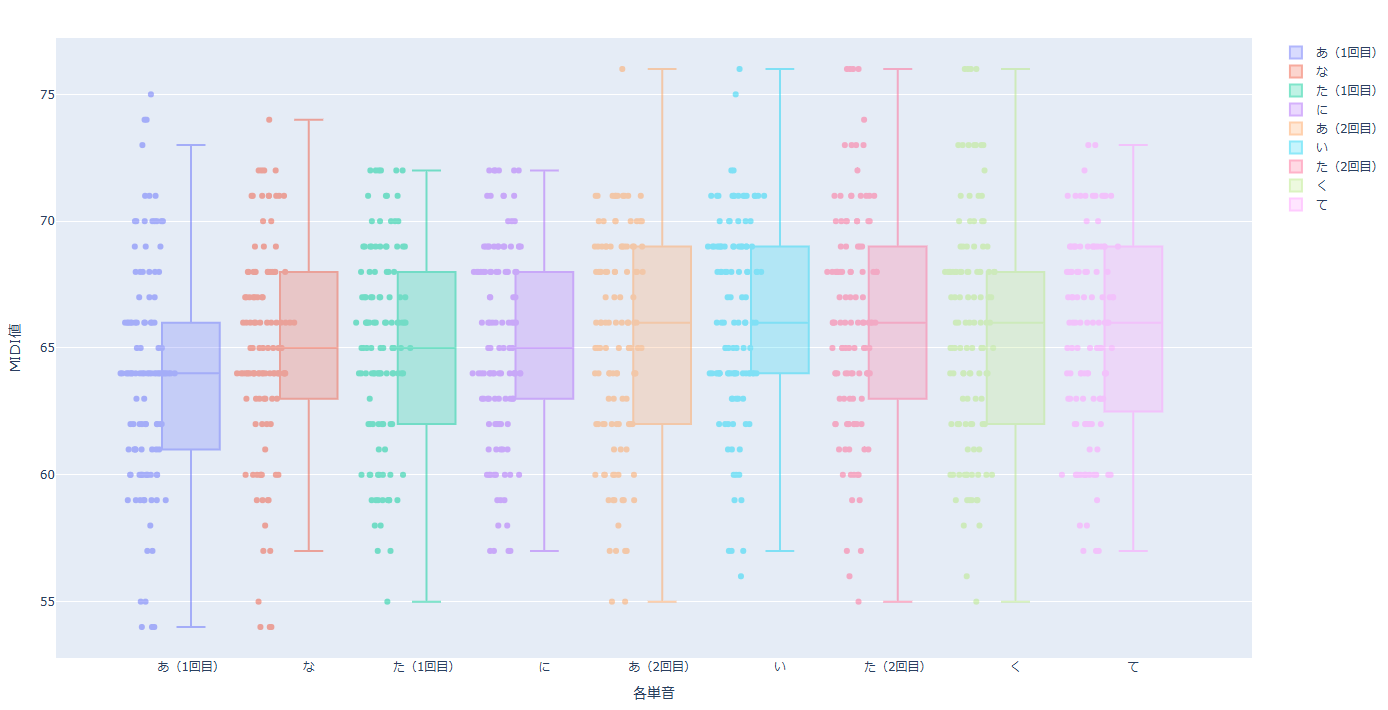
\includegraphics[width=\columnwidth]{fig/anata/midi/onna.png}
    \subcaption{“あなたにあいたくて”}
    \label{a_midi_onna}
  \end{minipage}
  \begin{minipage}{0.49\hsize}
    \centering
    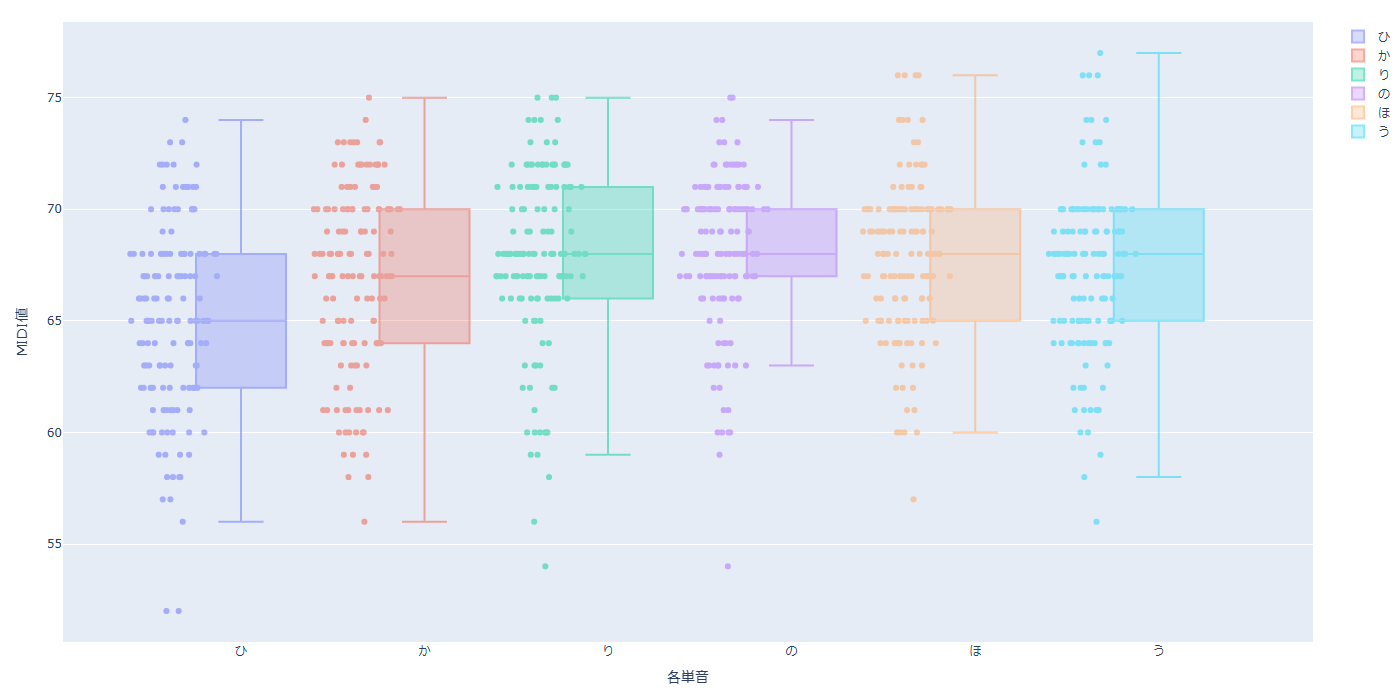
\includegraphics[width=\columnwidth]{fig/hikari/midi/onna.png}
    \subcaption{“ひかりのほう”}
    \label{h_midi_onna}
  \end{minipage}
  \caption{音高（MIDIナンバー）の女性の分布}
  \label{midi_onna}
\end{figure*}

\textbf{“あなたにあいたくて”での結果}\par
\figref{a_midi_otoko}により，「あ（2回目）」「た」「く」において，同フレーズ内で見れば広い音域をカバーしているが，\figref{a_midi_zentai}と比較すると，低音はあまりカバーできていないことがわかる．

\textbf{“ひかりのほう”での結果}\par
\figref{h_midi_onna}により，「の」において，箱やひげが他の単音と比べて狭いことから，かなりばらつきが少ないことがわかる．また，「ひ」「か」に関して低めの音が集まっているのがわかる．
また，「ひ」「か」「う」において，同フレーズ内で見れば広い音域をカバーしているが，\figref{h_midi_zentai}と比較すると，低音はあまりカバーできていないことがわかる．

\subsubsection{混合での結果}
\begin{figure*}[t]
  \centering
  \begin{minipage}{0.49\hsize}
    \centering
    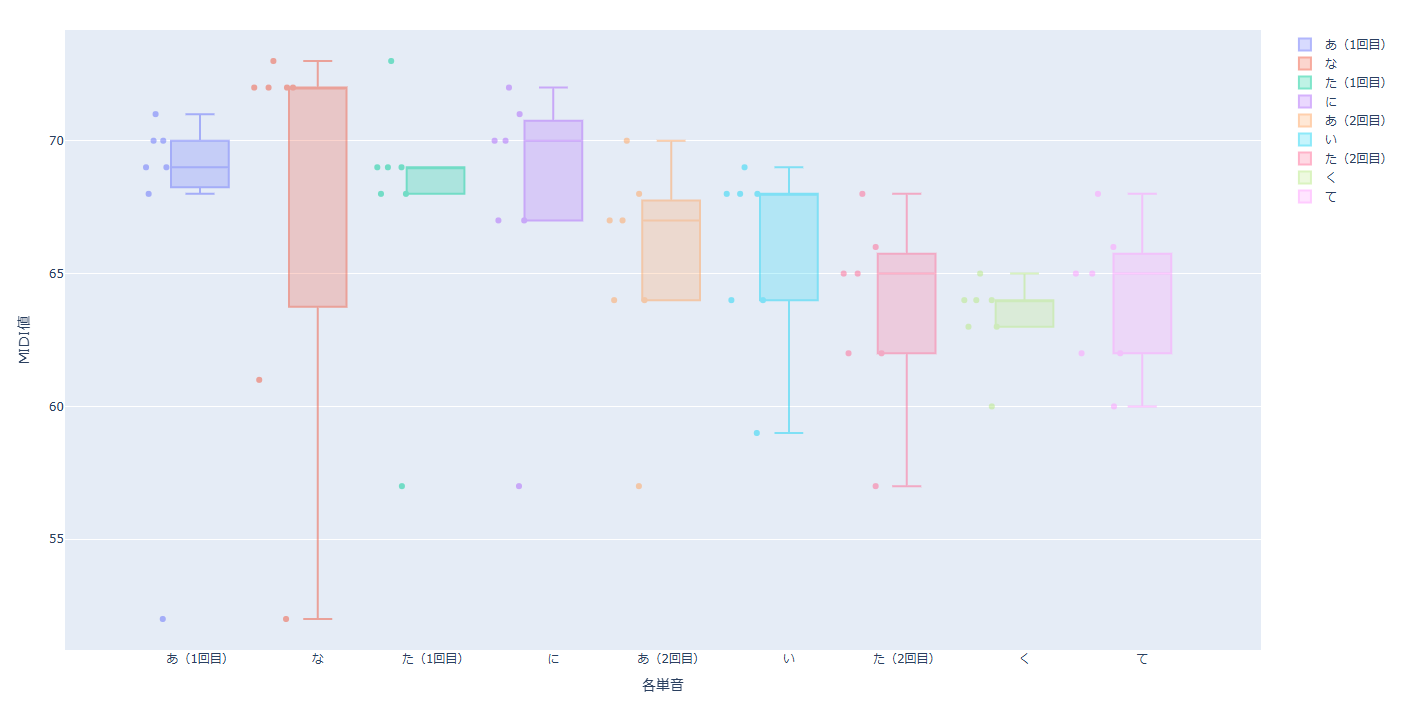
\includegraphics[width=\columnwidth]{fig/anata/midi/kongo.png}
    \subcaption{“あなたにあいたくて”}
    \label{a_midi_kongo}
  \end{minipage}
  \begin{minipage}{0.49\hsize}
    \centering
    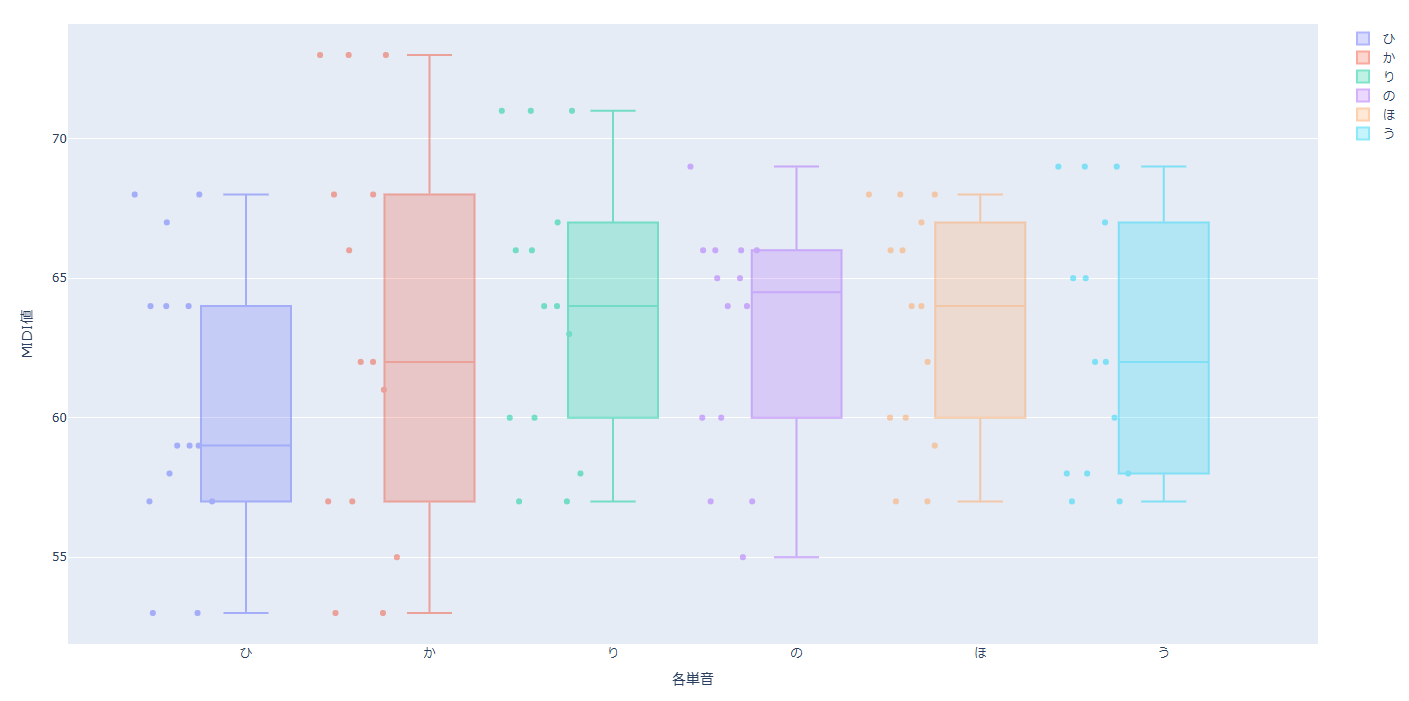
\includegraphics[width=\columnwidth]{fig/hikari/midi/kongo.png}
    \subcaption{“ひかりのほう”}
    \label{h_midi_kongo}
  \end{minipage}
  \caption{音高（MIDIナンバー）の混合の分布}

  \label{midi_kongo}
\end{figure*}

\textbf{“あなたにあいたくて”での結果}\par
\figref{a_midi_kongo}より，「あ（1回目）」や「た（1回目）」「く」において，箱の大きさがかなり小さいため，かなり偏りがあることがわかる．また，「な」において，ひげがかなり大きいことから，かなり広い音域をカバーしていることがわかる．しかし，\figref{a_midi_zentai}と比べると，そこまで広い音域をカバーしているとはいえない．

\textbf{“ひかりのほう”での結果}\par
\figref{h_midi_kongo}より，「か」や「う」の箱が大きいため，広い範囲の高さで歌われていると言える．しかし，\figref{h_midi_zentai}と比べると，そこまで広い音域をカバーしているとはいえない．

%6
\section{考察}
各フレーズについて，発話表現との比較，および秒数に換算したときの比較をまとめ，どのような特徴があるのかを考察していく．
\subsection{「あなたにあいたくて」フレーズについて}
\ref{sec:4}節より，「あなたにあいたくて」フレーズ全体の特徴として，歌唱タイミングは自由な傾向にあること，歌唱イントネーションも自由な傾向にあるが，特に「あ（1回目）」と「て」の，フレーズの最初と最後が他の単音と比べて低く歌われる傾向にあることがわかった．\par
また，男女での歌唱の違いについては，歌唱タイミングについて，男性は「あなた」「あいたくて」で発話タイミングとずれた歌唱傾向にある一方，女性は「あなたに」では崩し気味なものの「あいたくて」では発話タイミングと近いタイミングで歌われることが多い傾向にあることがわかる．また，歌唱イントネーションについては，男性は全体の歌唱イントネーションと似た傾向にあることがわかり，女性に関しては「い」が高めに歌われる傾向があることがわかった．また，タイミングとイントネーションの乖離について，女性の方がイントネーションの乖離が多いことがわかる．\par
さらに，発売日年別の歌唱の違いについては，1970年代，1980年代，1990年代の歌唱タイミングにおいて，かなり発話タイミングと近いタイミングで歌唱されていることがわかる．また，発話イントネーションについて，あまり発話イントネーションと一致する年代はなかった．特に，2010年代は，かなりばらつきがあったと考えられる．\par
また，「あなたにあいたくて」の表拍・裏拍の分布について，表拍で歌われることが多いことが確認できる．
さらに，全体および男女の音高分布において，男性の歌唱において，かなり広い音域をカバーしていることが読み取れた．
また，「あなたにあいたくて」の発話表現と歌唱表現の秒数比較について，全ての楽曲において発話表現よりも長い秒数をかけて歌われていることがわかる．

\subsection{「ひかりのほう」フレーズについて}
\ref{sec:4}節より，「ひかりのほう」フレーズ全体の特徴として，歌唱タイミングは比較的，発話タイミングと近しい場合もあると考えられる．一方，歌唱イントネーションは自由な傾向にあるが，特に「か」と「う」に関して，かなり広いイントネーションの位置で歌われていることがわかる．\par
また，男女での歌唱の違いについては，歌唱タイミングについて，男性は「か」「り」で発話タイミングとずれた歌唱傾向にある一方，女性は「か」「ほ」で発話タイミングとずれて歌われる傾向にあることがわかる．また，歌唱イントネーションについては，男性は全体の歌唱イントネーションと似た傾向にあることがわかり，女性に関しては「ひ」「か」が若干低めの分布にあることがわかった．また，タイミングとイントネーションの乖離について，どちらでもタイミング完全一致が複数個あることが確認できる．\par
さらに，発売日年別の歌唱の違いについては，そもそも2000年代からしか存在しないのが特徴の一つといえる．発話タイミングについて，「り」について，2000年代では歌唱タイミングより早いものが多いが，2010年代には遅いものが多いことが傾向としてとれる．また，発話イントネーションについて，あまり発話イントネーションと一致する年代はなく，どの年代も歌唱イントネーションと似たような分布になっていることがわかる．\par
また，「ひかりのほう」の表拍・裏拍の分布について，表拍で歌われることも多いが，裏拍開始での歌唱も多いことがわかる．\par
さらに，全体および男女の音高分布において，男性の歌唱において，かなり広い音域をカバーしていることが読み取れた．\par
また，「ひかりのほう」の発話表現と歌唱表現の秒数比較について，ほとんどの楽曲において発話表現よりも長い秒数をかけて歌われているが，一部の楽曲は発話表現よりも短い時間で歌われていることがわかった．

%7
%\section{結論}
%本研究では，発話表現と歌の表現を，「音での表現」という観点から比較し，両者に違いがあるのかを検討した．そのために，主に発話表現と歌唱表現との比較を行った．また，秒数（実時間）換算した発話表現・歌唱表現との比較も取り入れ，さらに新たな研究対象フレーズ「ひかりのほう」を追加し，研究の拡張を行った．
%結果を以下にまとめる．
%「あなたにあいたくて」は，全体ではあまり発話表現との一致は見られなかった．しかし，女性では歌唱タイミングにおいて「あいたくて」で発話表現と近しい傾向にあったことから，女性が歌唱者の際は「あいたくて」を伝えやすくするために，


%8
%\section{謝辞}
%本論文の執筆にあたり, 主指導教員である橋田光代准教授には, 研究に詰まった際のアドバイスや発表資料，論文執筆のご指導などいただいたことに心から感謝する．また，所属する橋田ゼミの皆様には

